\documentclass[12pt,letterpaper]{amsart}
\usepackage[letterpaper,margin=1in]{geometry}
\usepackage[T1]{fontenc}
\usepackage{amsmath,amssymb,amsthm,mathtools}
\usepackage{newtxtext,newtxmath}
\usepackage{booktabs,longtable,array,enumitem,tabularx,tikz}
\usetikzlibrary{arrows.meta,positioning}
\usepackage[hidelinks]{hyperref}
\usepackage{microtype}
\allowdisplaybreaks[2]
\numberwithin{equation}{section}
\newtheorem{theorem}{Theorem}[section]
\newtheorem{proposition}[theorem]{Proposition}
\newtheorem{lemma}[theorem]{Lemma}
\newtheorem{corollary}[theorem]{Corollary}
\theoremstyle{definition}
\newtheorem{definition}[theorem]{Definition}
\newtheorem{example}[theorem]{Example}
\newtheorem*{example*}{Example}
\theoremstyle{remark}
\newtheorem{remark}[theorem]{Remark}
\newcommand{\F}{F}
\newcommand{\G}{G}
\newcommand{\calH}{\mathcal H}
\newcommand{\calC}{\mathcal C}
\newcommand{\I}{\mathcal I}
\newcommand{\tr}{\operatorname{tr}}
\newcommand{\Irr}{\operatorname{Irr}}
\newcommand{\vol}{\operatorname{vol}}
\newcommand{\St}{\operatorname{St}}
\newcommand{\Ind}{\operatorname{Ind}}
\newcommand{\Hom}{\operatorname{Hom}}
\newcommand{\Supp}{\operatorname{supp}}
\newcommand{\Ad}{\operatorname{Ad}}
\newcommand{\diag}{\operatorname{diag}}
\newcommand{\Jac}{\operatorname{Jac}}
\newcommand{\PW}{\operatorname{PW}}
\newcommand{\triv}{\mathbf 1}
\newcommand{\EP}{\operatorname{EP}}
\newcommand{\ST}{\mathcal{ST}}
\newcommand{\Ann}{\operatorname{Ann}}
\newcommand{\Ext}{\operatorname{Ext}}
\newcommand{\ev}{\operatorname{ev}}
\title[A hitch-hiker's guide to invariant distributions]{A hitch-hiker's guide to invariant distributions on \\ $\mathrm{SL}_2$ over a $p$-adic field \\[0.6ex] Draft 4. Corrected and expanded version}
\author{David Joyner}
\email{wdjoyner@gmail.com}
\thanks{The original is an unpublished manuscript of the same title, dated November 2, 1994. This corrected and expanded version is dated November 24, 2026.}
\date{Original draft: 1994. Corrected and expanded draft: 2026}
\subjclass[2020]{22E50, 22E35, 11F70}
\keywords{Invariant distributions, $p$-adic $\mathrm{SL}_2$, trace Paley--Wiener theorem, principal series, supertempered virtual characters}
\begin{document}
\begin{abstract}
This AI-aided paper is a corrected and expanded version of notes written in 1994. Argon-Gemini, Sol-ChatGPT and Fable-Claude revised and extended the notes, and Sol-ChatGPT refereed two of the drafts. See the Acknowledgments and the revision log for details. The paper is an expository and research-oriented account of invariant distributions on $G=\mathrm{SL}_2(F)$, where $F$ is a non-archimedean local field of odd residue characteristic. Its theme is the difference between the operator-valued Fourier transform $f\mapsto\pi(f)$ and the trace transform $f\mapsto\tr\pi(f)$, which sees only the cocenter of the Hecke algebra. Every conjugation-invariant linear functional on the Hecke algebra is a distribution, so the invariant distributions form the algebraic dual of the trace Paley--Wiener space. In rank one this space has explicit coordinates: a Laurent polynomial on each family of principal series, and finitely many scalars at the reducible points. We prove that tempered traces determine all admissible traces algebraically but not continuously. We describe the invariant distributions that extend to holomorphic, smooth and Schwartz spectral spaces by the growth of their spectral moments. A distribution with finite Bernstein support is locally a finite combination of tempered characters, and we determine when its normalized restriction to the split torus is locally constant. We give a direct proof of Herb's classification of supertempered virtual characters in rank one and compare two splittings of the elliptic quotient. The results on admissibility and on supertempered characters assume that $F$ has characteristic zero. The results on the Schwartz space depend on Arthur's trace Paley--Wiener theorem. The source checks that remain are listed in the text.
\end{abstract}
\maketitle
\tableofcontents

\section{Introduction and scope}\label{sec:intro}
This section states the objectives of the paper, lists its principal results, describes its structure, and separates what is proved here from what is cited and from what remains open. It ends with the notation.

\subsection{Background and objectives}\label{sec:objectives}
The original notes were written to understand invariant distributions in the simplest non-abelian reductive $p$-adic group.  The rank-one case is especially attractive: the torus of diagonal matrices is one-dimensional, the principal-series characters are explicit, and the reducible principal series already illustrate the role of virtual characters.  These features also make $\mathrm{SL}_2(F)$ a useful point of comparison with genuine representations of metaplectic covers.

There is a conceptual distinction that controls the entire subject.  The map $f\mapsto\pi(f)$ is an \emph{operator-valued} Fourier transform.  Its traces $\Theta_\pi(f)=\tr\pi(f)$ are invariant spectral data, and do not determine the original test function $f$.  They determine instead its image in the \emph{invariant quotient} (also called the cocenter) of the Hecke algebra.  Once this is taken into account, the Bernstein--Deligne--Kazhdan theorem has a precise and efficient statement.

The objective is to describe invariant distributions on $G$ as linear functionals on spectral data, in a case where every object can be written down. Three points of view meet. The algebraic one uses Bernstein components, Grothendieck groups, the cocenter and the action of the Bernstein center. The analytic one uses the Schwartz space, spaces of holomorphic functions and their continuous duals. The geometric one uses orbital integrals, descent to the torus, the exceptional fibers of the spectrum and the elliptic representations. The elementary rank-one calculations connect the three.

\subsection{Principal results}\label{sec:results}
The main statements are the following. Each is proved in the paper from the classical inputs named in its hypotheses.
\begin{enumerate}[label=\arabic*.,leftmargin=*]
\item \emph{Invariant distributions are an algebraic dual.} The span of the convolution commutators equals the span of the conjugation differences $f-f^g$ (Lemma \ref{lem:conj}). Every linear functional on the Hecke algebra is continuous. With Kazhdan's density theorem this identifies the invariant distributions with the full algebraic dual of the trace Paley--Wiener space (Proposition \ref{prop:alg-dual}).
\item \emph{Normalized orbital integrals need not vanish at singular elements.} The normalized split orbital integral of $\mathbf 1_K$ is identically one on the regular units (Example \ref{ex:K}).
\item \emph{The geometry of the spectrum.} The support map to the Bernstein variety has doubled fibers, and the unitary dual is not Hausdorff at them (Proposition \ref{prop:endpoint-limits}). The admissible dual has a standard Borel structure (Proposition \ref{prop:borel-model}). The trace image of a block is a polynomial ring with two extra scalar coordinates (Proposition \ref{prop:algebraic-pw}).
\item \emph{Tempered traces determine admissible traces, but not continuously.} The restriction maps from admissible to unitary to tempered trace data are isomorphisms (Theorem \ref{thm:pwcomparison}). Evaluation at a non-tempered representation is not continuous for the smooth topology (Theorem \ref{thm:pwinstability}).
\item \emph{Three duality theories.} A functional on the Laurent polynomials extends to holomorphic functions on $\mathbb C^\times$, or to smooth functions on the circle, exactly when its moments grow at most exponentially, or at most polynomially (Theorems \ref{thm:laurent}, \ref{thm:three-duals}, \ref{thm:duality-moments} and \ref{thm:duality-holomorphic}). Eigenfunctionals and generalized eigenfunctionals of the Bernstein center are computed by a recurrence (Theorems \ref{thm:duality-eigen} and \ref{thm:duality-jets}).
\item \emph{Admissibility and descent.} A distribution with finite Bernstein support is, on each relatively compact open set, a finite combination of tempered characters (Theorem \ref{thm:local-interpolation}). It is therefore admissible (Theorem \ref{thm:finite-block-admissibility}). Its normalized restriction to the split torus extends to a locally constant function exactly when a condition on the trivial-orbit coefficients holds (Theorem \ref{thm:unramified-descent} and Corollary \ref{cor:descent}).
\item \emph{Supertempered distributions.} The supertempered virtual characters are spanned by the discrete series characters and the three differences of quadratic constituents (Theorem \ref{thm:herb-rank-one}). They give one of two natural splittings of the elliptic quotient (Theorem \ref{thm:twosplit}). The weak constant term of a finite-block distribution is its induced part (Theorem \ref{thm:decomp}).
\end{enumerate}
No claim of novelty is made for these statements. Most are rank-one cases of general theorems, and the purpose is to make them explicit.

\subsection{Structure of the paper}\label{sec:structure}
The literature review follows this introduction. Section \ref{sec:rep} is background on representations, the principal series and the Schwartz space. Section \ref{sec:spectral-geometry} describes the spectrum as a set, a topological space, a Borel space and an algebraic variety. Section \ref{sec:orbital} recalls orbital integrals and computes one of them. Section \ref{sec:cocenter} is the center of the paper: the trace transform, the cocenter, the trace Paley--Wiener theorem, and the comparison of the admissible, unitary, tempered and Schwartz trace images. Sections \ref{sec:tempered-duality} and \ref{sec:admissible-duality} describe the continuous duals of the tempered and the admissible spectral spaces. Section \ref{sec:descent} treats admissible distributions, descent to the torus and finiteness conditions. Section \ref{sec:supertemp} treats supertempered distributions. Section \ref{sec:summary} summarizes the results and the open problems. A glossary of technical terms comes before the Acknowledgments.

\subsection{Hypotheses, classical inputs and open questions}\label{sec:status}
Sections \ref{sec:rep}, \ref{sec:orbital} and the first part of Section \ref{sec:cocenter} allow any non-archimedean local field of odd residue characteristic, except where Kazhdan's density theorem is used (Remark \ref{rem:density-char}). Sections \ref{sec:spectral-geometry}, \ref{sec:descent} and \ref{sec:supertemp} assume that $F$ is a finite extension of $\mathbb Q_p$ with $p$ odd, because they use Harish-Chandra's regularity theory, the local character expansion and Herb's theorems. Everything in the paper concerns the rank-one group $\mathrm{SL}_2$. No statement is made for groups of higher rank, except for the quoted general theorems.

We distinguish results proved here, cited results, conditional identifications and open problems. The main cited results are the classification of the irreducible representations of $G$, the trace Paley--Wiener theorem \cite{BDK86}, the density theorem \cite{Ka86}, Arthur's trace Paley--Wiener theorem for Schwartz functions \cite{Ar94}, Harish-Chandra's regularity theorems \cite{HC99}, and the theorems of Casselman \cite{Ca77} and Herb \cite{He94}. A statement whose proof uses a source that has not been checked in detail says so, and the places where a check is outstanding are marked ``Remark 2026.$n$''.

The rank-one spectral models make the comparison of the three trace images explicit. Three questions remain open: the full topological identification of the Schwartz trace image and of the closed commutator subspace, admissibility and descent for distributions with infinite Bernstein support, and a criterion on the group for the analyticity of a spectral functional. They are discussed in Section \ref{sec:summary}.

\subsection{The running example}\label{sec:running}
The field $F=\mathbb Q_3$ is used as a running example. Here $q=3$, the uniformizer is $3$, and the square classes are represented by $1,2,3,6$. The table lists where the example appears.
\begin{center}\small
\begin{tabularx}{\linewidth}{@{}p{.37\linewidth}X@{}}\toprule
Topic & What is computed for $\mathbb Q_3$\\\midrule
Reducibility (Section \ref{sec:rep}) & The five reducible inducing characters $|\cdot|^{\pm1}$, $\eta_2$, $\eta_3$, $\eta_6$, and the exceptional unramified parameters $z\in\{\tfrac13,-1,3\}$\\
Complementary series (Section \ref{sec:rep}) & The interval $\tfrac13<z<1$ and its inverse\\
Spectrum (Section \ref{sec:spectral-geometry}) & The doubled fibers over $u=-2$ and $u=\tfrac{10}3$\\
Orbital integrals (Section \ref{sec:orbital}) & $\mathcal O_{a(t)}(\mathbf 1_K)=3^n$ at $t=1+3^n$\\
Trace coordinates (Section \ref{sec:cocenter}) & The polynomial $Q(u)=u^2-2$, with values $2$ and $\tfrac{82}9$ at the exceptional points\\
Moments and recurrences (Section \ref{sec:admissible-duality}) & The eigenfunctional with moments $3^n+3^{-n}$\\
Descent (Section \ref{sec:descent}) & The values $3^{-n}$ of $|t-t^{-1}|$ at $t=1+3^n$\\
Supertempered characters (Section \ref{sec:supertemp}) & The three differences $D_{\eta_2}$, $D_{\eta_3}$, $D_{\eta_6}$, and a combination of discrete series characters that descends\\\bottomrule
\end{tabularx}
\end{center}

\subsection{Notation and conventions}\label{sec:notation}
This subsection fixes the field, the group and its subgroups, the normalization of induction, and the main symbols. The table at the end collects the notation for later reference.

Let $F$ be a non-archimedean local field with residue characteristic different from $2$, ring of integers $\mathcal O$, maximal ideal $\mathfrak p$, a uniformizer $\varpi$, and residue-field cardinality $q$.  Write $v(\varpi)=1$ and $|x|=q^{-v(x)}$.  Fix an additive Haar measure on $F$ with $\vol(\mathcal O)=1$; Haar measures on other groups are specified as needed. Put
\[
\begin{aligned}
G&=\mathrm{SL}_2(F),\quad K=\mathrm{SL}_2(\mathcal O),\quad
A=\{a(t)=\diag(t,t^{-1}):t\in F^\times\},\\
N&=\left\{n(x)=\begin{pmatrix}1&x\\0&1\end{pmatrix}:x\in F\right\}.
\end{aligned}
\]
and $B=AN$.  The modular character satisfies $\delta_B(a(t))=|t|^2$.  The center is $Z(G)=\{\pm I\}$. We use \emph{normalized} parabolic induction throughout:
\begin{equation}\label{eq:induction}
I(\chi)=\Ind_B^G(\chi),\qquad
\chi(a(t))=\chi(t),
\end{equation}
where $\chi:F^\times\to\mathbb C^\times$ is a smooth quasicharacter. Here $\Ind$ denotes \emph{normalized} smooth induction: a function in the induced model satisfies $\phi(bg)=\delta_B(b)^{1/2}\chi(b)\phi(g)$ (with the usual right-translation action), not a Hilbert-space completion. Thus the modular factor is included \emph{once}. Let $G_{\rm reg}$ denote the regular semisimple set, $\calH(G)=C_c^\infty(G)$ the Hecke algebra, and $\calC(G)$ the Harish-Chandra Schwartz space.  In a formula involving a Weyl discriminant we write $\Delta_G$, never the letter $D$ (which is reserved for distributions).

\begin{center}\small
\begin{tabular}{@{}p{0.18\linewidth}p{0.73\linewidth}@{}}\toprule
Symbol & Meaning \\\midrule
$\widehat G_{\rm adm}$ & Irreducible smooth admissible representations, up to isomorphism \\
$\widehat G_{\rm temp}$ & Irreducible tempered representations, up to isomorphism \\
$R(G)$ & Complexified Grothendieck group of finite-length smooth $G$-representations \\
$\Theta_\pi$ & Distribution character $f\mapsto\tr\pi(f)$ \\
$\Delta_G(\gamma)$ & $\det(1-\Ad(\gamma)|_{\mathfrak g/\mathfrak g_\gamma})$ on $G_{\rm reg}$ \\
$\mathcal O_\gamma(f)$ & Orbital integral over $G_\gamma\backslash G$ \\
$\calH(G)_{\rm coc}$ & Cocenter $\calH(G)/[\calH(G),\calH(G)]$ \\
$\PW_{\rm tr}(G)$ & Image of the trace transform on $R(G)^*$ \\\bottomrule
\end{tabular}
\end{center}

\section*{Literature review}\label{sec:lit}
This section summarizes the works on which the paper depends and says how each one is used. It is divided at 1994, the date of the original notes.

\subsection*{Before 1994}
Gelfand and Graev \cite{GG63} gave explicit descriptions of the representations of $\mathrm{SL}_2$ over a locally compact non-archimedean field. Their work is the source of the principal-series parametrization recalled in Section \ref{sec:rep}.

Sally and Shalika computed the characters of the discrete series of $\mathrm{SL}_2$ \cite{SS68} and studied the Fourier transform of orbital integrals \cite{SS84}. These papers are the source of the explicit elliptic character values that lie behind Example \ref{ex:supertemp}.

Silberger's book \cite{Si79} is based on lectures of Harish-Chandra. It develops the Schwartz space, the constant term and the Eisenstein integral for a general reductive $p$-adic group. We cite it for the Schwartz space and its topology in Section \ref{sec:rep} and for the normalized constant term in Section \ref{sec:descent}. Casselman's notes \cite{Ca93} introduce admissible representations, parabolic induction and the Jacquet module. We cite them for these foundations.

Bernstein, Deligne and Kazhdan \cite{BDK86} characterize the image of the trace map on the Hecke algebra. The image consists of the linear forms on the Grothendieck group that are regular under unramified twisting and are supported at one compact open level. This is Theorem \ref{thm:BDK}, the central statement of Section \ref{sec:cocenter}. Kazhdan's paper \cite{Ka86} contains the density theorem. Section \ref{sec:cocenter} uses it to identify the cocenter with the quotient of the Hecke algebra by the kernel of the trace transform.

Clozel \cite{Cl91} treats invariant harmonic analysis on the Schwartz space. It is a reference for Subsection \ref{sec:schwartz}.

Arthur \cite{Ar93} introduced the elliptic tempered virtual characters attached to the $R$-group. He expected them to span the supertempered virtual characters. Herb \cite{He94} proved this. She also showed that a tempered virtual character is supertempered if and only if all of its weak constant terms vanish. Section \ref{sec:supertemp} rests on these two papers. Herb's paper appeared in 1994, the year of the original notes.

Arthur \cite{Ar94} proved a trace Paley--Wiener theorem for the Schwartz space, also in 1994. The trace map from the Schwartz space to a space of smooth functions on the parameters $(M,\sigma,r)$ is continuous, open and surjective. The statements about the Schwartz trace image in Sections \ref{sec:spectral-geometry}, \ref{sec:cocenter} and \ref{sec:tempered-duality} depend on this theorem.

Tadi\'c studied the topology of the unitary dual of a reductive group over a local field \cite{Ta83}. This is the source of the questions about the Fell topology and the Borel structure in Section \ref{sec:spectral-geometry}. His notes on $\mathrm{SL}(n)$ \cite{Ta92} describe the representations of $\mathrm{SL}(n)$ by restriction from $\mathrm{GL}(n)$.

Casselman \cite{Ca77} related the character of an admissible representation on contracting elements to the character of its Jacquet module. Rodier \cite{Ro75} related Whittaker models to the regular terms of the local character expansion. Keys \cite{Ke82} computed the $R$-groups of the reducible principal series, and Labesse and Langlands \cite{LL79} described the packets of $\mathrm{SL}_2$. Borel \cite{Bo76} identified the unramified block with the modules over the Iwahori--Hecke algebra, and Kottwitz \cite{Ko88} introduced the Euler--Poincar\'e function. Harish-Chandra introduced supertempered distributions for real groups \cite{HC83}. Section \ref{sec:supertemp} uses these works.

\subsection*{After 1994}
Waldspurger \cite{Wa03} wrote out Harish-Chandra's unpublished proof of the Plancherel formula for reductive $p$-adic groups. The formula expresses a Schwartz function in terms of the tempered representations. This article complements \cite{Si79} as a detailed reference for the Schwartz-space theory that Subsections \ref{sec:schwartzbackground} and \ref{sec:schwartz} only quote.

Schneider and Zink \cite{SZ07} study the category of nondegenerate modules over the Harish-Chandra Schwartz algebra. They construct functors of parabolic induction and restriction for this category, and show that the functors are exact and adjoint to each other on both sides. Their work gives an algebraic framework for the tempered theory sketched in Subsection \ref{sec:schwartz}.

Dat \cite{Da00} studies the group $K_0$ of the Hecke algebra of a reductive $p$-adic group by means of the Hattori--Stallings rank. This rank takes values in the cocenter \eqref{eq:cocenter}. The paper is a later development of the ideas around the cocenter and \cite{BDK86,Ka86}.

Adler, DeBacker, Sally and Spice \cite{ADSS11} derive the supercuspidal character formulas of $\mathrm{SL}_2$ announced in \cite{SS68} from the general theory of supercuspidal characters, and supply proofs.

Schneider and Stuhler \cite{SS97} proved that the Euler--Poincar\'e pairing is the elliptic pairing and gave a fixed-point formula for characters at elliptic elements. Korman \cite{Ko04} extended the formula to compact elements in rank one. Reeder \cite{Re01} related the elliptic space of Iwahori-spherical representations to elliptic representations of Weyl groups. Opdam and Solleveld \cite{OS13} computed extensions of tempered representations and recovered Arthur's inner product formula. Ciubotaru and He \cite{CH17,CH21} studied elliptic and rigid cocenters. Aubert and Plymen \cite{AP24} compared the character formulas of $\mathrm{SL}_2$ with the endoscopic character identities.

Harish-Chandra's lectures on admissible invariant distributions \cite{HC99} contain the regularity theorems and the local character expansion used in Sections \ref{sec:descent} and \ref{sec:supertemp}. DeBacker \cite{De02} proved homogeneity results that make the range of validity of the expansion precise. Aizenbud, Gourevitch and Sayag \cite{AGS15} studied distributions that are finite under the Bernstein center. They proved that the wave-front set of such a distribution lies in the nilpotent cone. The preprint \cite{CT26} concerns admissibility for the Bernstein center. No result of \cite{De02}, \cite{AGS15} or \cite{CT26} is used in a proof here.

Roche \cite{Ro98} constructed types for the principal series blocks of split groups and identified their Hecke algebras. Aubert, Baum, Plymen and Solleveld \cite{ABPS14,ABPS17,ABPS19} described blocks of the smooth dual by extended quotients. Section \ref{sec:spectral-geometry} compares its explicit description with theirs. Solleveld studied completions of Hecke algebras \cite{So19} and computed the Hochschild homology of the Hecke algebra and of the Schwartz algebra \cite{So24}. His survey \cite{So25} covers both. Hochschild homology in degree zero is the cocenter, so these works bear on the open question about the closed commutator subspace of the Schwartz algebra.

Section \ref{sec:supertemp} uses the fixed-point formulas of \cite{SS97,Ko04} in two proofs. Sections \ref{sec:spectral-geometry}, \ref{sec:cocenter} and \ref{sec:tempered-duality} use \cite{Ar94}, and Sections \ref{sec:descent} and \ref{sec:supertemp} use \cite{HC99}. The other works after 1994 are not used in a proof in this paper. They are listed to orient the reader.

\section{Representations: definitions and the rank-one families}\label{sec:rep}
This section is the background for the rest of the paper. It recalls smooth and admissible representations, the principal series and its points of reducibility, the quadratic characters of $F^\times$, and the Schwartz space. Nothing in it is new. The section fixes the normalizations that the later sections use.

\begin{definition}
A representation $(\pi,V)$ of $G$ is \emph{smooth} if every $v\in V$ is fixed by some open compact subgroup of $G$. It is \emph{admissible} if $\dim_{\mathbb C}V^J<\infty$ for every open compact $J\subset G$.  It is \emph{irreducible} if it has no proper nonzero $G$-stable subspace.  These notions do not require the homomorphism $G\to\operatorname{Aut}(V)$ to be continuous when $\operatorname{Aut}(V)$ is given the discrete topology: that stronger condition would force an open global kernel.
\end{definition}
\begin{example*}
The trivial representation of $G$ on $\mathbb C$ is smooth, admissible and irreducible.

The induced representation $I(\chi)$ of \eqref{eq:induction} is smooth by construction. It is also admissible. Let $J\subset G$ be open and compact. The Iwasawa decomposition $G=BK$ shows that the map $K\to B\backslash G/J$ is surjective. It factors through $K/(K\cap J)$, which is finite because $K\cap J$ is open in the compact group $K$. So $B\backslash G/J$ is finite. A $J$-fixed function in $I(\chi)$ is determined by its values on a set of representatives of $B\backslash G/J$. Hence $\dim I(\chi)^J\le|B\backslash G/J|<\infty$.

The representation of $G$ on $C_c^\infty(G)$ by right translation is smooth but not admissible. Its $J$-fixed vectors are the compactly supported functions on $G$ that are constant on the cosets $gJ$. This space is infinite-dimensional because $G/J$ is infinite.
\end{example*}
An irreducible unitary Hilbert-space representation of a reductive $p$-adic group has a dense space of smooth vectors, giving an irreducible admissible smooth representation.  This assertion is \emph{not} true for an arbitrary (reducible) unitary representation: an infinite-dimensional direct sum of trivial representations has infinite-dimensional fixed-vector spaces.

For $f\in\calH(G)$ define
\begin{equation}\label{eq:opFT}
\pi(f)v=\int_Gf(g)\pi(g)v\,dg,
\qquad \Theta_\pi(f)=\tr\pi(f).
\end{equation}
For admissible $\pi$, the operator $\pi(f)$ has finite rank and the trace is defined. Conjugation of $f$ does not change $\Theta_\pi(f)$.

\subsection{Principal series and reducibility}
This subsection recalls where the principal series $I(\chi)$ is reducible. The answer depends on the normalization of induction, so the statement is tied to \eqref{eq:induction}.

The Weyl element $w=\begin{psmallmatrix}0&-1\\1&0\end{psmallmatrix}$ identifies the inducing parameters $\chi$ and $\chi^{-1}$ at the level of semisimplified principal series.  One must not treat the resulting parameter quotient as though every point labeled a single irreducible representation.

\begin{theorem}[Standard rank-one reducibility criterion]\label{thm:reducibility}
Under the normalization \eqref{eq:induction}, $I(\chi)$ is reducible precisely when
\begin{equation}\label{eq:reducibility}
\chi=|\cdot|^{\pm1}\quad\text{or}\quad \chi^2=1,\ \chi\ne1.
\end{equation}
At $|\cdot|^{\pm1}$ the induced representation has constituents the trivial representation and the Steinberg representation (with the appropriate subrepresentation/quotient ordering).  For nontrivial quadratic $\chi$, the normalized unitary principal series splits into two inequivalent irreducible tempered constituents.
\end{theorem}
\begin{proof}[Source and normalization note]
This is the standard $\mathrm{SL}_2$ principal-series classification; see \cite{GG63,Si79,Ca93}.  The $|\cdot|^{\pm1}$ exceptions arise because the normalized induction \eqref{eq:induction} includes the modular factor $\delta_B^{1/2}=|\cdot|$ in its inducing model.  They must not be omitted when quoting a criterion originally formulated for an unnormalized induction.
\end{proof}

If $\chi$ is unitary and $I(\chi)$ is irreducible, it is tempered. The irreducible constituents at nontrivial quadratic characters, the Steinberg representation, and supercuspidal representations are also tempered; the trivial representation is not tempered.

With the normalization \eqref{eq:induction} the \emph{complementary series} consists of the representations
\begin{equation}\label{eq:complementary}
I(|\cdot|^s),\qquad 0<s<1 .
\end{equation}
They are irreducible and unitarizable, and they are not tempered. The Weyl symmetry $I(|\cdot|^s)\simeq I(|\cdot|^{-s})$ gives the same representations for $-1<s<0$. In terms of the parameter $z=\chi(\varpi)=q^{-s}$ of an unramified character, the complementary series is the interval
\[
q^{-1}<z<1
\]
together with its inverse $1<z<q$. At the endpoint $z=1$ the representation $I(1)$ is irreducible and tempered. At the endpoints $z=q^{\mp1}$ the induced representation is reducible, with constituents the trivial and Steinberg representations. Figure \ref{fig:parameters} shows these parameters. These paragraphs are a guide to the families, taken from the classification \cite{GG63,Ta92}. They are not a new proof of the classification of the unitary dual.
\begin{figure}[htbp]\centering
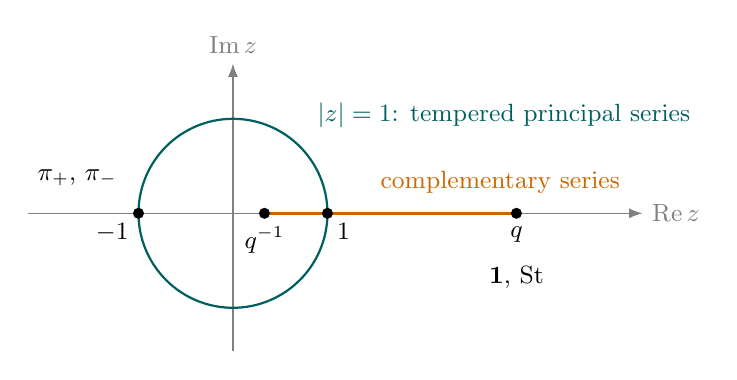
\begin{tikzpicture}[>=Latex,every node/.style={font=\small}]
\draw[->,gray] (-2.6,0)--(5.2,0) node[right]{$\operatorname{Re}z$};
\draw[->,gray] (0,-1.75)--(0,1.9) node[above]{$\operatorname{Im}z$};
\draw[thick,teal!75!black] (0,0) circle (1.2);
\draw[very thick,orange!80!black] (0.4,0)--(3.6,0);
\fill (-1.2,0) circle (2pt);\node[below left] at (-1.2,0) {$-1$};
\fill (1.2,0) circle (2pt);\node[below right] at (1.2,0) {$1$};
\fill (0.4,0) circle (2pt);\node[below] at (0.4,-.05) {$q^{-1}$};
\fill (3.6,0) circle (2pt);\node[below] at (3.6,-.05) {$q$};
\node[teal!75!black,anchor=west] at (0.95,1.25) {$|z|=1$: tempered principal series};
\node[orange!80!black,anchor=west] at (1.75,.4) {complementary series};
\node[anchor=north] at (3.6,-.55) {$\triv$, $\St$};
\node[anchor=east] at (-1.35,.45) {$\pi_+$, $\pi_-$};
\end{tikzpicture}
\caption{The unramified parameters $z=\chi(\varpi)\in\mathbb C^\times$, drawn for $q=3$. The Weyl symmetry is $z\mapsto z^{-1}$. The induced representation is reducible at $z=-1$ and at $z=q^{\pm1}$. The figure shows the parameter space of the unramified principal series, not the whole unitary dual.}\label{fig:parameters}
\end{figure}
\begin{example*}
Let $F=\mathbb Q_3$, so $q=3$. By Theorem \ref{thm:reducibility}, exactly five quasicharacters $\chi$ of $F^\times$ give a reducible $I(\chi)$. Two of them are the unramified characters $|\cdot|$ and $|\cdot|^{-1}$, which take the values $1/3$ and $3$ at the uniformizer $3$. The other three are the nontrivial quadratic characters. In the notation of Subsection \ref{sec:quad} below they are $\eta_2$, $\eta_3$ and $\eta_6$. The character $\eta_2$ is unramified, because $\mathbb Q_3(\sqrt2)$ is the unramified quadratic extension of $\mathbb Q_3$. The characters $\eta_3$ and $\eta_6$ are ramified. In the parameter $z$ of the unramified characters, the three exceptional points are $z=\tfrac13$, $z=3$ and $z=-1$, and the complementary series is $\tfrac13<z<1$. For instance $z=3^{-1/2}$ is the complementary series representation $I(|\cdot|^{1/2})$.
\end{example*}

\subsection{Quadratic characters and examples}\label{sec:quad}
The reducibility criterion \eqref{eq:reducibility} involves the quadratic characters of $F^\times$. This subsection lists them and fixes their names.

Because the residue characteristic is odd,
\begin{equation}\label{eq:squareclasses}
F^\times/(F^\times)^2=\{1,\varepsilon,\varpi,\varepsilon\varpi\}
\end{equation}
for any fixed nonsquare unit $\varepsilon$.  For $\tau\in F^\times/(F^\times)^2$, the associated quadratic character is
\begin{equation}\label{eq:hilbert}
\eta_\tau(x)=(x,\tau)_F,
\end{equation}
where $(\ ,\ )_F$ is the quadratic Hilbert symbol.  It is equivalently the character whose kernel is the norm group from $F(\sqrt\tau)$.  It is \emph{not} characterized by a universal condition $\eta_\tau(\tau)=1$.
\begin{example}
For $F=\mathbb Q_3$, choose $\varepsilon=2$. The square classes are represented by $1,2,3,6$.  The ramified quadratic character $\eta_3$ satisfies
$\eta_3(3)=(3,3)_3=-1$.  For $F=\mathbb Q_5$, $\varepsilon=2$ also works, and the representatives are $1,2,5,10$.
\end{example}


\subsection{From matrix coefficients to the Schwartz theory}\label{sec:schwartzbackground}
This subsection recalls matrix coefficients, the classes of representations defined through them, and the Harish-Chandra Schwartz space. These notions are used in Sections \ref{sec:cocenter} and \ref{sec:supertemp}.

Let $(\pi,V)$ be smooth and admissible, and let $(\widetilde\pi,\widetilde V)$ denote its smooth contragredient.  A \emph{matrix coefficient} is a function
\[
m_{v,\widetilde v}(g)=\langle\pi(g)v,\widetilde v\rangle.
\]
A supercuspidal irreducible representation is characterized by compact support of its matrix coefficients modulo the center (equivalently, vanishing Jacquet modules for proper parabolics). Because the center of $\mathrm{SL}_2(F)$ is finite, compact support modulo the center means compact support.  An irreducible square-integrable representation has square-integrable matrix coefficients modulo the center; its character contributes discretely to Plancherel measure.  Supercuspidal representations are square-integrable, but the Steinberg representation illustrates why the converse fails.
\begin{example*}
For the trivial representation we have $V=\widetilde V=\mathbb C$, and every matrix coefficient is a constant function on $G$. A nonzero constant function is not compactly supported. It is also not square-integrable, because the noncompact group $G$ has infinite Haar measure. So the trivial representation is neither supercuspidal nor square-integrable. This agrees with the table at the end of this subsection.
\end{example*}

The Harish-Chandra Schwartz space is modeled on estimates involving a height function $\sigma:G\to\mathbb R_{\ge0}$ and the spherical function $\Xi$.  One may choose, for example, a $K$-bi-invariant proper length comparable to
$\log_q\max\{\|g\|,\|g^{-1}\|\}$, where the matrix norm is the maximum absolute value of the entries. The defining seminorms are
\begin{equation}\label{eq:seminorms}
p_N(f)=\sup_{g\in G}\frac{|f(g)|\,(1+\sigma(g))^N}{\Xi(g)}
\qquad(N\ge0).
\end{equation}
The topology is defined in two steps \cite{Si79,Wa03}. For an open compact subgroup $J$ let $\calC(G/\!/J)$ be the space of $J$-bi-invariant functions $f$ on $G$ with $p_N(f)<\infty$ for every $N$. The seminorms $p_N$ make it a Fr\'echet space. The Schwartz space is the union of these spaces, with the locally convex inductive-limit topology:
\begin{equation}\label{eq:schwartz-limit}
\calC(G)=\bigcup_J\calC(G/\!/J)=\varinjlim_J\calC(G/\!/J).
\end{equation}
A \emph{tempered distribution} is a continuous linear functional on $\calC(G)$. By the definition of the inductive-limit topology, a linear functional $T$ on $\calC(G)$ is continuous if and only if its restriction to each $\calC(G/\!/J)$ is continuous. This means that for each $J$ there are $N$ and $C$, which may depend on $J$, with $|T(f)|\le C\,p_N(f)$ for all $f\in\calC(G/\!/J)$. It is this \emph{topology}, rather than just the decay of a single function, that governs a tempered distribution.
\begin{example*}
Evaluation at the identity, $T(f)=f(1)$, is a tempered distribution. Indeed $\Xi(1)=1$ and $\sigma(1)=0$, so $|f(1)|\le p_0(f)$ on every $\calC(G/\!/J)$. The functional $f\mapsto\int_Gf(g)\,dg$ is defined on $\calH(G)$ and is the character of the trivial representation. It does not extend continuously to $\calC(G)$, because the trivial representation is not tempered.
\end{example*}

\begin{center}\small
\begin{tabular}{@{}p{0.28\linewidth}p{0.28\linewidth}p{0.32\linewidth}@{}}\toprule
Family & Tempered? & What it illustrates \\\midrule
Unitary irreducible principal series & Yes & Continuous tempered spectrum \\
Two summands of a quadratic principal series & Yes & Reducibility and $R$-group matching \\
Supercuspidal irreducibles & Yes & Compactly supported matrix coefficients modulo center \\
Steinberg & Yes, square-integrable & Discrete series not supercuspidal \\
Nontrivial complementary series & No & Unitary need not mean tempered \\
Trivial representation & No & A constituent at $|\cdot|^{\pm1}$ \\\bottomrule
\end{tabular}
\end{center}

\subsection{What the dual parameterization does and does not say}
This subsection describes how the principal series is organized into one-parameter families. It also says where a parameter fails to name a single irreducible representation.

Fixing the restriction of a quasicharacter to $\mathcal O^\times$ leaves a one-dimensional family of unramified twists, naturally parametrized by $z=\chi(\varpi)\in\mathbb C^\times$.  Inversion takes $(\chi|_{\mathcal O^\times},z)$ to $(\chi^{-1}|_{\mathcal O^\times},z^{-1})$. At a quadratic point, however, two irreducibles occur, and at the parameters $|\cdot|^{\pm1}$ there are composition factors that are not obtained by treating the principal-series family as a disjoint collection of simple points. The Bernstein component or Grothendieck-group description avoids such ambiguity.
\begin{example*}
Take the family of unramified characters, so that $\chi|_{\mathcal O^\times}=1$ and $\chi(x)=z^{v(x)}$ with $z=\chi(\varpi)$. The character $|\cdot|^s$ has $z=q^{-s}$. By Theorem \ref{thm:reducibility}, the reducibility points in this family are $z=q^{-1}$, $z=q$ and $z=-1$. The first two are the characters $|\cdot|$ and $|\cdot|^{-1}$, where the constituents are the trivial and Steinberg representations. The third is the unramified quadratic character, where there are two tempered constituents. Inversion $z\mapsto z^{-1}$ exchanges $z=q^{-1}$ and $z=q$, and it fixes $z=-1$. Inversion also fixes $z=1$, the trivial character, and there $I(\chi)$ is irreducible.
\end{example*}

% Insertable section for Draft 3; requires amsmath, amssymb, amsthm, booktabs,
% tabularx, tikz (arrows.meta,positioning), and theorem/proposition/remark environments.
\section{The geometry, topology, and Borel structure of the representation spectrum}\label{sec:spectral-geometry}
The admissible, unitary, and tempered duals of $G=\mathrm{SL}_2(F)$ encode different kinds of spectral information. This section makes their relationship explicit in rank one. We assume that $F$ is a finite extension of $\mathbb Q_p$, with $p>2$, residue cardinality $q$, valuation $v$, uniformizer $\varpi$, and ring of integers $\mathcal O$. The absolute value is $|a|=q^{-v(a)}$. Our main example is the unramified principal series. Its exceptional fibers explain why the Bernstein variety alone cannot parameterize the trace transform.

\subsection{Four structures on the spectrum}\label{subsec:four-structures}
Write $\widehat G_{\rm ad}$ for the irreducible smooth admissible dual, $\widehat G_u$ for the irreducible unitary dual (identified with its smooth vectors), and $\widehat G_{\rm temp}$ for the tempered dual. We have inclusions
\[\widehat G_{\rm temp}\subseteq\widehat G_u\subseteq\widehat G_{\rm ad}.\]
The following structures answer different questions.
\begin{center}\small
\begin{tabularx}{\linewidth}{@{}p{.23\linewidth}XX@{}}\toprule
Structure & Purpose & Information retained\\\midrule
Standard Borel structure & Direct integrals and measurable representation theory & Measurable sets of irreducibles\\
Fell topology & Convergence and weak containment & Limits of unitary representations\\
Bernstein variety & Algebraic organization of supercuspidal support & Regular dependence on unramified twists\\
Extended quotient & Enhanced spectral parameters & Extra labels at exceptional parameters\\\bottomrule
\end{tabularx}\end{center}
A standard Borel space is a measurable space isomorphic to a Borel subset of a Polish space. It need not be uncountable or isomorphic to the real line. The Fell topology is a topology on the unitary dual, not on arbitrary nonunitarizable smooth representations. The Bernstein variety is an algebraic variety, component by component, and is not generally the space of irreducibles itself. In the unramified block, for instance, the trivial and Steinberg representations have identical supercuspidal support but different temperedness properties.

\subsection{Supercuspidal support and exceptional fibers}\label{subsec:exceptional-fibers}
Let $B=AN$ be the upper triangular Borel subgroup, with $A=\{a(t)=\operatorname{diag}(t,t^{-1}):t\in F^\times\}$. Write $I(\chi)=\operatorname{Ind}_B^G(\chi)$ for normalized smooth induction; the transformation law includes $\delta_B(a(t))^{1/2}=|t|$. Fix a smooth character $\xi$ of $\mathcal O^\times$. The characters extending it are
\[\chi_{\xi,z}(\varpi^n a)=z^n\xi(a),\qquad z\in\mathbb C^\times.\]
The Weyl involution acts by $(\xi,z)\mapsto(\xi^{-1},z^{-1})$. Inertial equivalence identifies supercuspidal pairs up to conjugacy and unramified twist. The Bernstein variety of the corresponding component is $X_{\mathfrak s}=T_{\mathfrak s}/W_{\mathfrak s}$, where $T_{\mathfrak s}$ is the twist torus and $W_{\mathfrak s}$ preserves the inertial class of the inducing character. The support map $\beta:\widehat G_{\rm ad}^{\mathfrak s}\to X_{\mathfrak s}$ records the Weyl orbit of the actual inducing character, not just its restriction to units.

For the unramified block ($\xi=1$), $T_{\mathfrak s}=\mathbb C^\times$ and $W_{\mathfrak s}=\{1,w\}$ with $wz=z^{-1}$. The coordinate $u=z+z^{-1}$ identifies the quotient with $\mathbb A^1_{\mathbb C}$. Indeed $z^n+z^{-n}$ satisfies the recurrence $P_{n+1}=uP_n-P_{n-1}$ with $P_0=2$, $P_1=u$. Thus $\mathbb C[z,z^{-1}]^W=\mathbb C[u]$.

We use the classical rank-one reducibility and unitarity classification as input (see \cite{SS68,Ta92}; precise source checks remain in the verification note). With this normalization, $I(\chi)$ is reducible precisely for $\chi=|\cdot|^{\pm1}$ or nontrivial quadratic $\chi$. The former have the trivial and Steinberg representations as composition factors, each with multiplicity one. The latter split into two inequivalent tempered constituents. In particular $I(1)$ is irreducible. These statements concern smooth induction, not a choice of Hilbert norm at a nonunitary inducing parameter.
\begin{center}\small
\begin{tabularx}{\linewidth}{@{}lllX@{}}\toprule
$z$ & $u$ & Fiber size & Irreducibles\\\midrule
Generic & Generic & 1 & Principal series\\
$1$ & $2$ & 1 & $I(1)$\\
$-1$ & $-2$ & 2 & $\pi_+,\pi_-$ (tempered)\\
$q,q^{-1}$ & $q+q^{-1}$ & 2 & $\mathbf 1,\mathrm{St}$\\\bottomrule
\end{tabularx}\end{center}
Thus the support map has two doubled fibers. The Bernstein center acts by the same scalar on the two members of either fiber, whereas a trace functional can distinguish them.
\begin{figure}[htbp]\centering
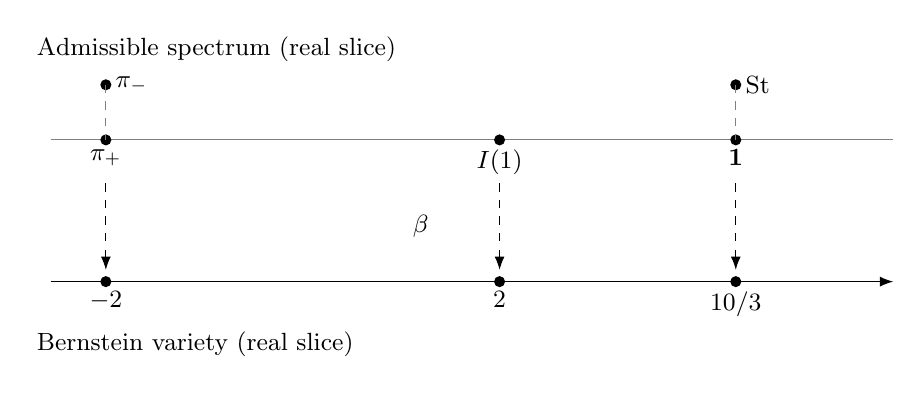
\begin{tikzpicture}[>=Latex,x=1cm,y=1cm,every node/.style={font=\small}]
\node[anchor=west] at (0,3.4) {Admissible spectrum (real slice)};
\draw[gray] (.3,2.25)--(11,2.25);
\foreach \x/\lab in {1/{\pi_+},6/{I(1)},9/{\mathbf1}} {\fill (\x,2.25) circle(2pt);\node[below] at (\x,2.25) {$\lab$};}
\fill (1,2.95) circle(2pt) node[right] {$\pi_-$};
\fill (9,2.95) circle(2pt) node[right] {$\mathrm{St}$};
\draw[gray,dashed] (1,2.95)--(1,2.25);\draw[gray,dashed] (9,2.95)--(9,2.25);
\foreach \x in {1,6,9} {\draw[->,dashed] (\x,1.7)--(\x,.6);}
\node at (5,1.15) {$\beta$};
\draw[->] (.3,.45)--(11,.45);
\foreach \x/\lab in {1/{-2},6/{2},9/{10/3}} {\fill (\x,.45) circle(2pt) node[below] {$\lab$};}
\node[anchor=west] at (0,-.35) {Bernstein variety (real slice)};
\end{tikzpicture}
\caption{Support fibers for $F=\mathbb Q_3$. The drawing records fiber cardinalities, not the Fell topology or the entire complex variety.}\label{fig:bernstein-fibers}
\end{figure}

\subsection{The three types of principal-series components}\label{subsec:three-types}
The restriction to units determines which Weyl elements preserve the inertial class. Consequently the classification reduces to three cases.
\begin{center}\small
\begin{tabularx}{\linewidth}{@{}llXX@{}}\toprule
Type & Condition & Variety & Doubled fibers\\\midrule
I & $\xi^2\ne1$ & $\mathbb C^\times$ & None\\
II & $\xi^2=1,\ \xi\ne1$ & $\mathbb C^\times/W$ & $z=\pm1$\\
III & $\xi=1$ & $\mathbb C^\times/W$ & $z=-1$, $\{q,q^{-1}\}$\\\bottomrule
\end{tabularx}\end{center}
In Type I the Weyl involution exchanges the two different unit-character families, so choosing one representative gives the entire twist torus without a further quotient. There are no reducibility points and the unitary and tempered parameters form a circle. In Type II the two quadratic extensions of $\xi$ give two split principal series. The unitary and tempered parameters are a closed interval with both endpoints replaced by two points. In Type III the complementary series $I(|\cdot|^s)$, $0<s<1$, and the trivial representation supplement the tempered spectrum. The Steinberg representation is tempered. These descriptions are set-theoretic until the topology is considered below.

For $p>2$, $F^\times/(F^\times)^2$ has four elements. The Hilbert symbol gives the quadratic characters $\eta_d(t)=(t,d)_F$. Over $\mathbb Q_3$ the nontrivial square classes are $2,3,6$; over $\mathbb Q_5$ they are $2,5,10$. In both examples $\eta_2$ is unramified, and the other two are ramified. For instance $(3,3)_3=-1$, whereas $(5,5)_5=1$. These follow from $(p,p)_p=(-1)^{(p-1)/2}$. Each field has three nontrivial quadratic inducing characters and hence six irreducible tempered constituents in the corresponding exceptional fibers. A ramified quadratic unit character and the trivial unit character therefore supply all three quadratic reducibility parameters.

\subsection{The Fell topology and doubled endpoints}\label{subsec:fell-model}
For unitary representations the Fell topology records weak containment. We use the equivalent topology on the irreducible spectrum of $C^*(G)$, with basic norm-open sets $\{\pi:\|\pi(a)\|>c\}$ for $a\in C^*(G)$ and $c\ge0$. In the unitary principal series $z=e^{i\theta}$, the support coordinate is $u=2\cos\theta$. The complementary series has $u=q^s+q^{-s}$, $0<s<1$. The expected topology in Type III is an interval $[-2,q+q^{-1}]$ with each endpoint doubled. The two copies of each endpoint are distinct but have every neighborhood meeting the same adjacent interval.

\begin{proposition}[Fell convergence from finite-rank traces]\label{prop:fell-trace}
Suppose $\pi_j$ are irreducible unitary representations and $\tau_1,\ldots,\tau_m$ are irreducible unitary representations. Assume that for each $h\in C_c^\infty(G)$,
\[\operatorname{tr}\pi_j(h)\longrightarrow\sum_{i=1}^m\operatorname{tr}\tau_i(h),\]
and that for every compact open subgroup $J$ the dimensions $\dim\pi_j^J$ are uniformly bounded (eventually in $j$). Then $\pi_j\to\tau_i$ in the Fell topology for each $i$.
\end{proposition}
\begin{proof}
Fix $i$ and a basic neighborhood $\|\tau_i(a)\|>c$. Approximate $a$ in the full $C^*$ norm by $h\in C_c^\infty(G)$ so closely that $\|\tau_i(h)\|>c+\epsilon$ and $\|a-h\|<\epsilon$ for some $\epsilon>0$. Choose $J$ so that $h$ is $J$-bi-invariant. For a positive integer $n$, the element $b_n=(h^**h)^{*n}$ (convolution power) is $J$-bi-invariant. Its image is positive, has rank at most $\dim\pi_j^J\le D$, and satisfies
\[D\|\pi_j(h)\|^{2n}\ge\operatorname{tr}\pi_j(b_n)\longrightarrow\sum_k\operatorname{tr}\tau_k(b_n)\ge\|\tau_i(h)\|^{2n}.\]
Here the final inequality holds because the positive operator on the finite-dimensional fixed-vector space has its norm as an eigenvalue. Taking $n$ large enough and then $j$ sufficiently far along the net gives $\|\pi_j(h)\|>c+\epsilon$ (reduce $\epsilon$ first if needed). The norm approximation gives $\|\pi_j(a)\|>c$. Finite intersections of these neighborhoods yield convergence.
\end{proof}

\begin{proposition}[Endpoint limits]\label{prop:endpoint-limits}
Subject to the rank-one classification above, a net of generic unitary principal-series parameters approaching a nontrivial quadratic parameter converges in the Fell topology to both constituents. A net of complementary-series parameters $s\to1$ converges to both $\mathbf1$ and $\mathrm{St}$ in the full unitary dual.
\end{proposition}
\begin{proof}
In the compact picture, $I(\chi_{\xi,z})|_K$, for $K=\mathrm{SL}_2(\mathcal O)$, is independent of $z$. For any compact open $J$, replace it by $J\cap K$ to obtain a uniform bound for the fixed-vector dimensions. For $h$ compactly supported and bi-invariant under a compact open subgroup of $K$, the trace is a Laurent polynomial in $z$: on the finite-dimensional fixed-vector space the Iwasawa decomposition introduces only finitely many valuation powers on the compact support. Therefore the trace converges to the trace of the entire induced module at the limiting parameter. Trace additivity for its finite composition series gives the sum of the two endpoint traces. All representations in that sum are unitarizable. Proposition~\ref{prop:fell-trace} applies. This argument does not require continuity of the complementary-series Hilbert inner products at the endpoint.
\end{proof}

\begin{figure}[htbp]\centering
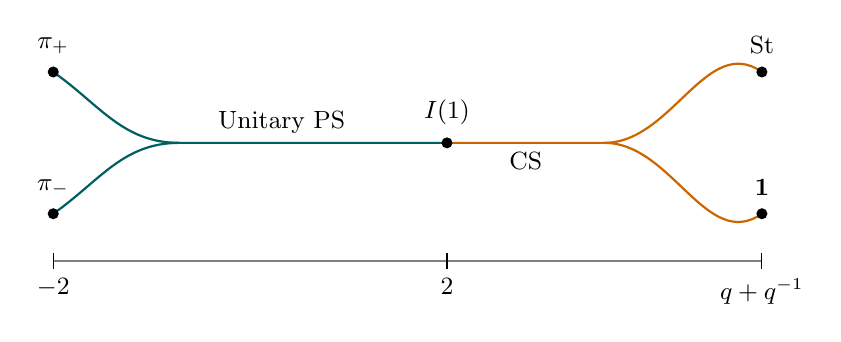
\begin{tikzpicture}[x=1cm,y=1cm,every node/.style={font=\small}]
\draw[teal!75!black,thick] (1,2.6) to[out=-35,in=180] (2.6,1.7)--(6,1.7);
\draw[teal!75!black,thick] (1,.8) to[out=35,in=180] (2.6,1.7);
\draw[orange!80!black,thick] (6,1.7)--(8,1.7) to[out=0,in=145] (10,2.6);
\draw[orange!80!black,thick] (8,1.7) to[out=0,in=-145] (10,.8);
\foreach \x/\y/\lab in {1/2.6/{\pi_+},1/.8/{\pi_-},6/1.7/{I(1)},10/2.6/{\mathrm{St}},10/.8/{\mathbf1}} {\fill (\x,\y) circle(2pt) node[above=3pt] {$\lab$};}
\node[above] at (3.9,1.7) {Unitary PS};\node[below] at (7,1.7) {CS};
\draw[gray] (1,.2)--(10,.2);\foreach \x/\lab in {1/{-2},6/{2},10/{q+q^{-1}}} {\draw (\x,.1)--(\x,.3);\node[below] at (\x,.1) {$\lab$};}
\end{tikzpicture}
\caption{Doubled-endpoint model for the full unramified unitary block. The forks indicate common limits, not ordinary Hausdorff branches. PS denotes principal series and CS complementary series.}\label{fig:fell-model}
\end{figure}
The endpoint convergence just proved implies non-Hausdorffness at both pairs in the full unitary dual. It does not imply that the Steinberg representation is nonisolated in the tempered dual: there the complementary series is absent. In the tempered block the expected model is the interval $[-2,2]$ with its left endpoint doubled, together with an isolated Steinberg point.

\begin{remark}[Remark 2026.1: exact topology]\label{rem:exact-fell}
For a full homeomorphism theorem it remains to exclude all other limits and verify the block topology. One route is to use a Bernstein type $(J,\lambda)$ and its Hecke algebra, together with the continuity of the central character on the unitary spectrum. A central element of the type algebra acts by a scalar on the finite-dimensional type space. Localizing with its type idempotent should force convergence of the support coordinate wherever a Fell limit exists. This, together with the endpoint proof, the $T_1$ property and separation of distinct support parameters, gives the proposed model. The required type-algebra and block-localization details are left for a subsequent verification. In Type I the analogous model is a circle; in Type II both endpoints of $[-2,2]$ are doubled. Normalized intertwining operators give an alternative route to the topology and to constituent labels.
\end{remark}

\subsection{Standard Borel structure}\label{subsec:standard-borel}
A measurable parameterization is easier to construct than a topological one. Let $E_{\mathfrak s}$ denote the finite set of doubled support parameters. Set
\[Y_{\mathfrak s}=(X_{\mathfrak s}\setminus E_{\mathfrak s})\sqcup\bigsqcup_{x\in E_{\mathfrak s}}\beta^{-1}(x).\]
Give the first summand its complex Borel structure and the finite fibers their discrete structures.
\begin{proposition}[A standard Borel model]\label{prop:borel-model}
The above parameterization and the singleton supercuspidal blocks define a standard Borel structure on $\widehat G_{\rm ad}$.
\end{proposition}
\begin{proof}
Each complex torus quotient in the three cases is a complex affine curve, and deleting finitely many points leaves a standard Borel space. Each exceptional fiber is finite. Smooth unit characters form a countable union of finite character groups of the finite quotients $\mathcal O^\times/(1+\varpi^n\mathcal O)$. There are countably many supercuspidals: they are unitary and their isolated classes in the second-countable unitary spectrum form a countable set (using the usual isolation theorem for supercuspidals). Alternatively one can use countability of Bernstein blocks. The group has no nontrivial unramified characters, so each supercuspidal block is a singleton. A countable disjoint union of standard Borel spaces is standard Borel.
\end{proof}
For a doubled-endpoint interval its Borel structure is exactly that obtained by adjoining two discrete points to the open interval at each doubled end. Indeed its finitely many endpoint singletons are Borel, and the ordinary open interval is open with its usual topology. Conversely each open set restricts to an ordinary open subset of the interior and to a subset of the finite endpoints. Thus the Borel structure forgets the non-Hausdorff convergence information. Once the exact Fell models in Remark~\ref{rem:exact-fell} are established, and the countable block decomposition is checked to be Borel, compatibility with the Fell Borel structure follows. This isolates the outstanding step in the original Tadi\'c-component question.

\subsection{Extended quotients and correcting cocharacters}\label{subsec:extended-quotient}
The modern geometric description of the smooth dual provides a natural refinement of the support map. For a finite group $W$ acting on a torus $T$, define
\[\widetilde T=\{(t,w)\in T\times W:wt=t\},\qquad T//W=\widetilde T/W,\]
where $v(t,w)=(vt,vwv^{-1})$. The extended quotient of the second kind replaces the element $w$ by an irreducible representation of the stabilizer:
\[(T//W)_2=\{(t,\rho):t\in T,\ \rho\in\widehat{W_t}\}/W,\quad W_t=\{w:wt=t\}.\]
The action on $\rho$ is transport by conjugation. For inversion on $\mathbb C^\times$, the nonidentity element fixes exactly $1$ and $-1$, so $T//W\cong(T/W)\sqcup\{e_+,e_-\}$. The ordinary projection doubles the fibers at $u=2$ and $-2$. In Type II this agrees with the cardinalities of the support fibers. In Type III it does not: the extra point at $u=2$ must instead map to $q+q^{-1}$, if it labels Steinberg. The point $e_-$ can label one quadratic constituent, with the other on the ordinary component. This gives an explicit set-theoretic bijection and corrected support map. It is not a canonical choice of constituent labels.

Aubert, Baum, Plymen and Solleveld establish extended-quotient descriptions for principal-series blocks of split reductive groups, including disconnected centers under the stated residual-characteristic hypotheses \cite[Sections 15, 18--19]{ABPS17}. Their correcting cocharacters explain why the projection to the ordinary quotient need not coincide with supercuspidal support. In this rank-one example the correcting map on the isolated Steinberg label can be modeled by $h(a)=a^2$ evaluated at $a=q^{1/2}$, followed by inversion quotient. This sends $1$ to the orbit of $q$. The other pieces use the identity correction (constant cocharacter $1$). This explicit model reproduces the support map; a canonical identification with the enhanced Langlands parameters requires additional choices and verification.
\begin{figure}[htbp]\centering
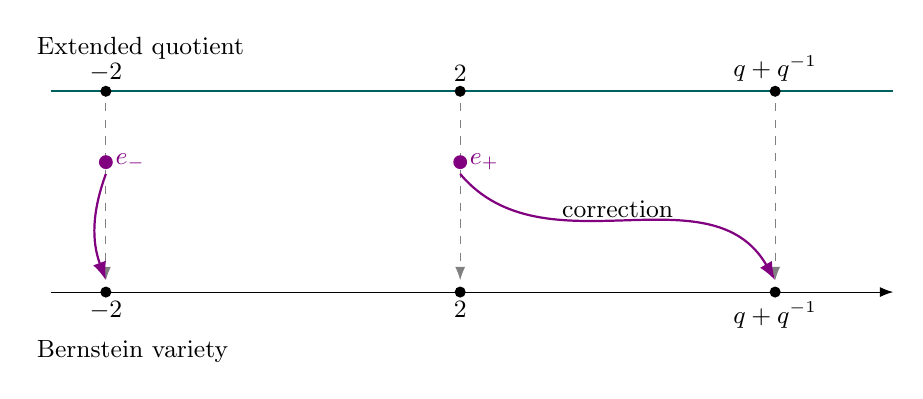
\begin{tikzpicture}[>=Latex,x=1cm,y=1cm,every node/.style={font=\small}]
\node[anchor=west] at (0,3.5) {Extended quotient};
\draw[thick,teal!75!black] (.3,2.95)--(11,2.95);
\foreach \x/\lab in {1/{-2},5.5/{2},9.5/{q+q^{-1}}} {\fill (\x,2.95) circle(2pt) node[above] {$\lab$};\draw[gray,->,dashed] (\x,2.8)--(\x,.55);}
\fill[violet] (1,2.05) circle(2.5pt) node[right] {$e_-$};
\fill[violet] (5.5,2.05) circle(2.5pt) node[right] {$e_+$};
\draw[->,violet,thick] (1,1.9) to[out=-110,in=110] (1,.55);
\draw[->,violet,thick] (5.5,1.9) to[out=-50,in=120] (9.5,.55);
\node at (7.5,1.45) {correction};
\draw[->] (.3,.4)--(11,.4);
\foreach \x/\lab in {1/{-2},5.5/{2},9.5/{q+q^{-1}}} {\fill (\x,.4) circle(2pt) node[below] {$\lab$};}
\node[anchor=west] at (0,-.35) {Bernstein variety};
\end{tikzpicture}
\caption{A corrected support map for Type III. The isolated label $e_+$ is sent to the support of Steinberg, not to $2$. The diagram is not a Fell homeomorphism.}\label{fig:correcting-map}
\end{figure}

The Weyl stabilizer and the Knapp--Stein $R$-group need not agree. The latter governs the endomorphism algebra of unitary parabolic induction. In the present examples the nontrivial $R$-group has order two; a choice of normalized self-intertwiner with square one labels the constituents by its two eigenvalues.
\begin{center}\small
\begin{tabular}{@{}lll@{}}\toprule
Unitary character & Weyl stabilizer & $R$-group\\\midrule
Generic & $1$ & $1$\\
Trivial & $\mathbb Z/2\mathbb Z$ & $1$\\
Nontrivial quadratic & $\mathbb Z/2\mathbb Z$ & $\mathbb Z/2\mathbb Z$\\\bottomrule
\end{tabular}\end{center}
In particular the stabilizer at $z=1$ is not evidence of reducibility of $I(1)$. An extended quotient with its disjoint-union topology cannot encode the common Fell limits of the exceptional constituents.

\subsection{Polynomial trace data and exceptional coordinates}\label{subsec:pw-coordinates}
Let $\mathcal H(G)=C_c^\infty(G)$ with convolution and fixed Haar measure. Its trace transform at an admissible irreducible $\pi$ is $\operatorname{tr}\pi(f)$, not the operator $\pi(f)$. Traces annihilate convolution commutators and hence factor through the Hecke cocenter. The algebraic trace Paley--Wiener theorem of Bernstein, Deligne and Kazhdan \cite{BDK86} characterizes the allowable trace functionals on the Grothendieck group of finite-length smooth representations.

For the unramified family put $P_f(z)=\operatorname{tr}I(\chi_{1,z})(f)$. By the compact-picture argument in Proposition~\ref{prop:endpoint-limits}, this is a Laurent polynomial. Weyl-related modules have the same semisimplification, so their traces agree. Hence $P_f(z)=Q_f(z+z^{-1})$, with $Q_f\in\mathbb C[u]$. Additivity gives
\begin{align}
Q_f(-2)&=\operatorname{tr}\pi_+(f)+\operatorname{tr}\pi_-(f),\label{eq:quadratic-sum}\\
Q_f(q+q^{-1})&=\operatorname{tr}\mathbf1(f)+\operatorname{tr}\mathrm{St}(f).\label{eq:steinberg-sum}
\end{align}
These are conditions on sums, not equalities of constituent traces.
\begin{proposition}[Polynomial uniqueness]\label{prop:poly-uniqueness}
The traces of $f$ on generic irreducible unramified unitary principal series determine its traces on the complementary series and its total induced traces throughout the complex unramified family.
\end{proposition}
\begin{proof}
Those traces determine $Q_f$ on $(-2,2)$, and a polynomial vanishing there is zero. Evaluate the same polynomial at $u=q^s+q^{-s}$ for the complementary series, or at any complex $u$ for the induced family. At the doubled fibers this recovers only the sums in \eqref{eq:quadratic-sum} and \eqref{eq:steinberg-sum}.
\end{proof}
For example $Q(u)=u^2-2$ corresponds to $z^2+z^{-2}$. Its values on the complementary series would be $q^{2s}+q^{-2s}$. Its value at the quadratic point is $2$, but that value alone does not distinguish the two constituent traces.

Introduce independent candidate coordinates
\begin{align*}
d_-(f)&=\operatorname{tr}\pi_+(f)-\operatorname{tr}\pi_-(f),\\
d_{\rm St}(f)&=\operatorname{tr}\mathrm{St}(f)-\operatorname{tr}\mathbf1(f).
\end{align*}
Together $(Q_f,d_-(f),d_{\rm St}(f))$ determine every irreducible trace in the block. For instance the first quadratic trace is $(Q_f(-2)+d_-(f))/2$, and the Steinberg trace is $(Q_f(q+q^{-1})+d_{\rm St}(f))/2$.
\begin{proposition}[Algebraic spectral coordinates]\label{prop:algebraic-pw}
Assuming the algebraic trace Paley--Wiener theorem in its usual good-functional formulation, the unramified block of the trace image is isomorphic as a vector space to
\[\operatorname{PW}_{\rm ad}^{\mathfrak s}\cong\mathbb C[u]\oplus\mathbb C^2.\]
\end{proposition}
\begin{proof}
Injectivity of the coordinate description follows from the preceding formulas. For surjectivity define a functional on the irreducible basis of the complex Grothendieck group using the polynomial at generic points and the half-sum and half-difference formulas at the doubled fibers. Extend by zero outside the unramified block. Its value on every normalized induction from $A$ is regular in the twisting parameter: it is either $Q(z+z^{-1})$ or zero. Induction from $G$ imposes no further twisting condition since $G$ has no nontrivial unramified characters. The functional vanishes outside a finite set of Bernstein components, and in the unramified block all constituents have Iwahori-fixed vectors (the Iwahori type for the unramified principal block). Thus it satisfies the finite-level support and regularity requirements of the good-functional theorem. That theorem realizes it as the trace of a test function. This is a specialization of the cited theorem, not an independent proof of the general theorem.
\end{proof}
The same argument gives $\mathbb C[z,z^{-1}]$ in Type I and $\mathbb C[u]\oplus\mathbb C^2$ in Type II, with differences at the two quadratic points. For the finite-level support in the ramified cases one uses the corresponding principal-series type. In the unramified block restriction to the unitary dual loses no trace information: the generic polynomial is determined on the circle and both members of each exceptional fiber are unitary. Thus the compactly supported unitary trace image has the same coordinates. This is not a claim that arbitrary continuous functions on the unitary dual extend to regular spectral functions.

\subsection{Schwartz trace data and spectral distributions}\label{subsec:schwartz-pw}
Arthur's Schwartz trace Paley--Wiener theorem \cite[Theorem, p.~174]{Ar94} describes trace data using triples $(M,\sigma,r)$, with $\sigma$ square-integrable modulo center and $r$ in the appropriate (possibly extended) $R$-group. His map from the Schwartz space to its spectral image is continuous, open and surjective. For a fixed rank-one torus family the identity-intertwiner trace is smooth on the unitary parameter circle; at a quadratic point the nonidentity intertwiner gives the difference trace. The Steinberg representation contributes separately through $M=G$. In particular the tempered trace space is not simply the space of continuous scalar functions on the Fell dual: unequal constituent traces are allowed, and the smooth function records the total induced trace.

\begin{proposition}[Rank-one Schwartz spectral model]\label{prop:schwartz-pw}
With Arthur's spectral topology restricted to the unramified block and a choice of normalized quadratic self-intertwiner, the block is modeled by
\[\operatorname{PW}_{\rm temp}^{\mathfrak s}\cong C^\infty(S^1)^W\oplus\mathbb C^2.\]
The two scalar coordinates are the quadratic difference trace and the Steinberg trace.
\end{proposition}
\begin{proof}
In Arthur's parameter set the identity $R$-element gives the unitary twist circle modulo Weyl equivalence. Smoothness means smoothness on the circle before quotienting. At $z=-1$ the nonidentity $R$-element gives an isolated parameter (the fixed-point twist space has dimension zero). The Steinberg representation gives another isolated parameter because $G$ has no nontrivial unramified twists. There are no other discrete-series parameters in the unramified block. For the order-two intertwiner normalized to be an involution, its trace against the operator $I(\chi)(f)$ is the difference of the two constituent traces. The identity trace at $-1$ is their sum. Arthur's invariance and smoothness requirements on these pieces are precisely the Weyl invariance of the circle function and unrestricted values on the isolated coordinates. The finite-support condition is automatic on these finitely many pieces. His theorem then gives the asserted image with the quotient topology: on the compact circle the seminorms are the ordinary uniform derivative seminorms, and on the isolated points they are absolute values. This uses the rank-one $R$-group classification and Arthur's theorem, not a new general Schwartz Paley--Wiener proof.
\end{proof}
The corresponding Type I model is $C^\infty(S^1)$, and Type II has the two independent quadratic differences instead of the Steinberg coordinate. For a Weyl-invariant smooth function in angular coordinates the odd derivatives vanish at $0$ and $\pi$. There is no matching of individual quadratic constituent traces to these derivatives; the value of the smooth total trace is their sum.

The continuous dual of the displayed Fr\'echet space is
\[\big(C^\infty(S^1)^W\big)'\oplus\mathbb C^2\cong\mathcal D'(S^1)^W\oplus\mathbb C^2.\]
The isomorphism extends a functional by composing with the averaging projection $g(z)\mapsto(g(z)+g(z^{-1}))/2$. In Fourier coordinates, distributions have polynomially bounded coefficients, including an arbitrary constant coefficient. Indeed continuity bounds the functional by finitely many derivative seminorms, which gives a polynomial bound on its values on $z^n$. Conversely Fourier coefficients of a smooth function decrease faster than every power, so pairing with a polynomially bounded sequence converges absolutely and defines a continuous functional. Weyl invariance identifies coefficients at $n$ and $-n$; it does not eliminate $n=0$.

Every such functional pulls back to a continuous invariant distribution under the trace map. Conversely a continuous invariant distribution factors through this spectral space if it annihilates the kernel of the trace map; openness of Arthur's map then proves continuity of the induced functional. Identifying that kernel with the appropriate closed commutator space is a separate density statement. For a countable locally convex direct sum of block spaces, its continuous dual is a product of block duals; this assertion depends on using the direct-sum topology, not a product topology on the test space. These distinctions are important when passing from a single block to the full Schwartz space.

\subsection{Supertempered virtual characters and research agenda}\label{subsec:geometry-agenda}
The exceptional coordinates suggest an application to Section 9 of the original research program. At a quadratic point the virtual character $\Theta_{\pi_+}-\Theta_{\pi_-}$ is the nonidentity-intertwiner trace. It detects the difference coordinate, whereas the total induced character detects the sum. The normalized Jacquet module of each constituent has the same character of $A$: the geometric lemma gives two copies of the quadratic inducing character for the whole induced representation, and the two constituents each have a nonzero Jacquet module by Frobenius reciprocity and their principal-series realization. Thus the virtual difference has zero normalized Jacquet character. Its weak constant term also vanishes. This makes it a natural example for the study of elliptic tempered virtual characters and supertemperedness. It does not by itself prove literal vanishing on all nonelliptic elements, or identify supertemperedness with support on the elliptic set. The appropriate character estimates and definitions must be checked separately.
\begin{figure}[htbp]\centering
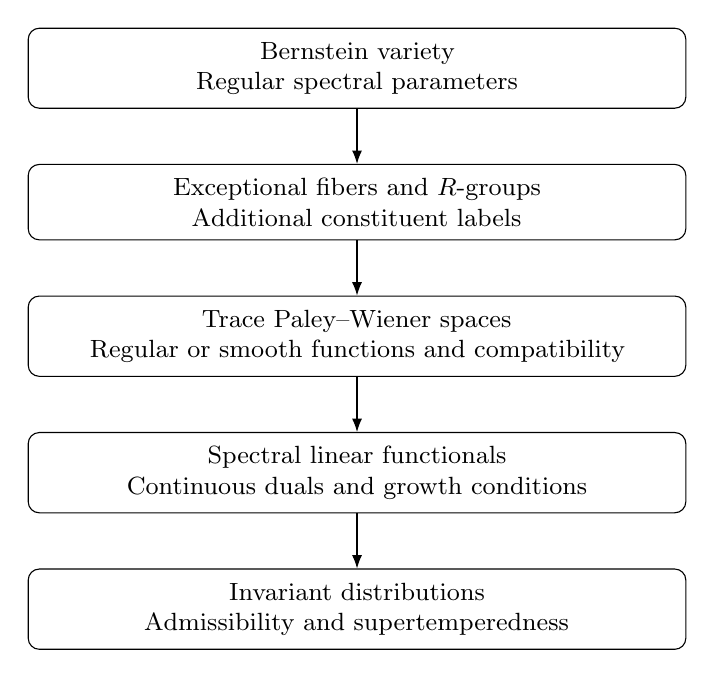
\begin{tikzpicture}[>=Latex,node distance=7mm,every node/.style={font=\small},stage/.style={draw,rounded corners,align=center,text width=8cm,inner sep=5pt}]
\node[stage] (a) {Bernstein variety\\ Regular spectral parameters};
\node[stage,below=of a] (b) {Exceptional fibers and $R$-groups\\ Additional constituent labels};
\node[stage,below=of b] (c) {Trace Paley--Wiener spaces\\ Regular or smooth functions and compatibility};
\node[stage,below=of c] (d) {Spectral linear functionals\\ Continuous duals and growth conditions};
\node[stage,below=of d] (e) {Invariant distributions\\ Admissibility and supertemperedness};
\draw[->] (a)--(b);\draw[->] (b)--(c);\draw[->] (c)--(d);\draw[->] (d)--(e);
\end{tikzpicture}
\caption{Dependencies of the geometric approach to invariant distributions. The last step requires the appropriate density, descent and growth results.}\label{fig:geometry-dependencies}
\end{figure}

The resulting research agenda is as follows. The classification of the three types, the standard Borel model, polynomial uniqueness and the finite-rank endpoint convergence argument are the first steps. Next verify the complete Fell homeomorphism theorem and compatibility of the Borel structures using types. Compare the extended quotient labeling with the canonical enhanced Langlands parameterization, including the correcting cocharacters. Check the good-functional and Schwartz spectral hypotheses in the cited sources in detail, including all normalizations. Finally apply the coordinate models to the analytic growth conditions, descent and supertempered virtual characters of the later sections. The obstruction to a full classification of invariant tempered distributions is not the finite exceptional fibers but the global topology and the kernel of the trace map. Figure~\ref{fig:geometry-dependencies} displays these dependencies.

\subsection{Literature and verification note}\label{subsec:geometry-literature}
The early foundations are the explicit rank-one representation theory of Gel'fand--Graev and Sally--Shalika, the topology of the dual studied by Tadi\'c, and the algebraic trace Paley--Wiener theorem of Bernstein--Deligne--Kazhdan. Arthur's 1994 Schwartz theorem supplies the topological trace result. After 1994, the type theory of Roche \cite{Ro98} and the extended-quotient program of Aubert, Baum, Plymen and Solleveld \cite{ABPS14,ABPS17,ABPS19} give a geometric interpretation of the principal-series classification. The last of these references concerns inner forms of $\mathrm{GL}_n$ and $\mathrm{SL}_n$ and is a useful comparison rather than a prerequisite for rank one.

The author-hosted version of \cite{ABPS17}, dated September 13, 2018, was consulted, particularly Section 19 and equations (136)--(138). The text of Arthur's theorem on p.~174 and the nonarchimedean proof on pp.~177--179 were consulted; the PDF screenshot retrieval timed out. The bibliography of Arthur's paper confirms the citation of \cite{BDK86}, but the full original good-functional theorem and the precise classical rank-one classification references were not independently checked in this pass. The polynomial and finite-rank convergence arguments above are independent derivations conditional only on their explicitly stated inputs. The exact Fell model is a research item, not an established homeomorphism in this section. The algebraic and Schwartz coordinate propositions are specializations of the cited general results, with the indicated rank-one and type-theoretic inputs still requiring a full source-level audit before publication.


\section{Orbital integrals, characters, and a singular-limit calculation}\label{sec:orbital}
This section recalls orbital integrals and the character formulas on the split torus. It then computes one normalized orbital integral near the singular elements $\pm I$. The computation shows that such integrals need not vanish there.

An orbital integral averages a test function over the conjugacy class of a fixed element $\gamma$. For regular semisimple $\gamma$ the centralizer $G_\gamma$ is a maximal torus, and the conjugacy class is closed in $G$ and is identified with $G_\gamma\backslash G$. So for $f\in\calH(G)$ the integrand below has compact support on $G_\gamma\backslash G$.

For $\gamma\in G_{\rm reg}$ let
\[
\mathcal O_\gamma(f)=\int_{G_\gamma\backslash G} f(x^{-1}\gamma x)\,d\dot x,
\qquad
F_f^T(\gamma)=|\Delta_G(\gamma)|^{1/2}\mathcal O_\gamma(f)
\]
when $\gamma$ belongs to the regular part of a maximal torus $T$.  Compatible invariant measures are understood.  The Weyl integration formula reads
\begin{equation}\label{eq:weyl}
\int_G f(g)\,dg=\sum_{[T]}\frac{1}{|W(G,T)(F)|}
\int_{T_{\rm reg}} |\Delta_G(t)|^{1/2}F_f^T(t)\,dt.
\end{equation}
The sum runs over $G(F)$-conjugacy classes of maximal $F$-tori; the rational Weyl-group order is retained explicitly.  It should not be silently replaced by $2$ in every elliptic term.

For $a(t)=\diag(t,t^{-1})$, we compute directly from the two root spaces that
\begin{equation}\label{eq:disc}
\Delta_G(a(t))=(1-t^2)(1-t^{-2})=-(t-t^{-1})^2,
\qquad |\Delta_G(a(t))|^{1/2}=|t-t^{-1}|.
\end{equation}
For the split torus, the normalized principal-series character on a regular element has the familiar form
\begin{equation}\label{eq:pschar}
\Theta_{I(\chi)}(a(t))=\frac{\chi(t)+\chi(t)^{-1}}{|t-t^{-1}|},
\end{equation}
while its regular elliptic character is zero.  The formula is for the character of the \emph{whole induced representation}; at a reducible point this character is the sum of the constituent characters.

\begin{example}[The normalized orbital integral need not vanish at $\pm I$]\label{ex:K}
We first rewrite the split normalized orbital integral of an arbitrary $f\in\calH(G)$. By the Iwasawa decomposition $G=ANK$, the quotient $A\backslash G$ is parametrized by the elements $n(y)k$, and the invariant measure is $dy\,dk$, with $\vol(\mathcal O)=\vol(K)=1$. So for regular $t$
\[
\mathcal O_{a(t)}(f)=\int_F\int_Kf\bigl(k^{-1}n(y)^{-1}a(t)\,n(y)k\bigr)\,dk\,dy .
\]
Multiplying the matrices gives
\begin{equation}\label{eq:conj-n}
n(y)^{-1}a(t)\,n(y)=a(t)\,n\bigl((1-t^{-2})y\bigr).
\end{equation}
Substitute $x=(1-t^{-2})y$. The Jacobian is $dy=|1-t^{-2}|^{-1}dx$. The discriminant factor is $|t-t^{-1}|=|t|\,|1-t^{-2}|$ by \eqref{eq:disc}, so the two factors combine:
\[
\frac{|t-t^{-1}|}{|1-t^{-2}|}=|t|=\delta_B(a(t))^{1/2}.
\]
Therefore
\begin{equation}\label{eq:FfA}
F_f^A(a(t))=\delta_B(a(t))^{1/2}\int_F\int_K f\bigl(k^{-1}a(t)n(x)k\bigr)\,dk\,dx .
\end{equation}
The factor $|\Delta_G(a(t))|^{1/2}$, which vanishes at $t=\pm1$, has been cancelled exactly by the Jacobian, which blows up there. The right-hand side of \eqref{eq:FfA} is defined for every $t\in F^\times$.

Now let $f=\mathbf 1_K$. The integrand does not depend on $k$. The matrix $a(t)n(x)$ has entries $t$, $tx$, $0$, $t^{-1}$. It lies in $K$ if and only if $t\in\mathcal O^\times$ and $x\in\mathcal O$. Hence
\begin{equation}\label{eq:FK}
F_{\mathbf 1_K}^A(a(t))=
\begin{cases}
1,&|t|=1,\ t\ne\pm1,\\
0,&|t|\ne1.
\end{cases}
\end{equation}
The vanishing for $|t|\ne1$ can also be seen directly: an element of $K$ has trace in $\mathcal O$, while $|t+t^{-1}|>1$. Thus along regular $t\to1$ the normalized orbital integral is \emph{identically one}, not zero.  The vanishing factor $|\Delta_G(a(t))|^{1/2}$ is compensated by the growth of the unnormalized orbital integral near the singular locus. For $F=\mathbb Q_3$ and $t=1+3^n$ we have $|t-t^{-1}|=3^{-n}$, so $\mathcal O_{a(t)}(\mathbf 1_K)=3^n$. Consequently the image of $f\mapsto F_f^A$ cannot be described as all compactly supported Weyl-invariant locally constant functions vanishing at $\pm1$.

The result agrees with the trace transform. By \eqref{eq:adj} below, $\Theta_{I(\chi)}(f)=\int_A\chi(a)F_f^A(a)\,da$, where the Haar measure on $A\simeq F^\times$ gives $\mathcal O^\times$ volume one. With \eqref{eq:FK} this gives $\Theta_{I(\chi)}(\mathbf 1_K)=\int_{\mathcal O^\times}\chi(t)\,d^\times t$, which is $1$ if $\chi$ is unramified and $0$ otherwise. On the other hand $\Theta_{I(\chi)}(\mathbf 1_K)=\dim I(\chi)^K$, and by $G=BK$ this dimension is $1$ for unramified $\chi$ and $0$ for ramified $\chi$. So the trace polynomial of $\mathbf 1_K$ in the unramified block is the constant $1$.
\end{example}

The local behavior of orbital integrals near singular elements is controlled by Shalika germs, not by the Weyl-discriminant factor alone.  Conversely, an arbitrary Weyl-invariant function on the regular split torus need not arise from an orbital integral with all the desired global and singular-germ properties.  We therefore use orbital integrals to explain character formulas, \emph{not} as an unproved surjectivity theorem for the full spectral Paley--Wiener space.

\section{The trace Fourier transform and the invariant quotient}\label{sec:cocenter}
This section is the center of the paper. It defines the trace transform, shows that it is not injective, and states the trace Paley--Wiener theorem of Bernstein, Deligne and Kazhdan, which describes its image. It then explains how an invariant distribution defines a functional on that image, and what changes for the Schwartz space.

Define the trace transform
\begin{equation}\label{eq:trace-map}
\mathcal F_{\rm tr}:\calH(G)\longrightarrow R(G)^*,\qquad
\mathcal F_{\rm tr}(f)([\pi])=\Theta_\pi(f),
\end{equation}
extending additively over finite-length representations. Here $R(G)$ denotes the \emph{complexified} Grothendieck group.

\begin{proposition}[Noninjectivity on the full Hecke algebra]\label{prop:kernel}
The trace transform \eqref{eq:trace-map} is not injective.
\end{proposition}
\begin{proof}
For $g\in G$ put $f^g(x)=f(g^{-1}xg)$.  Since the character distributions are invariant, $\Theta_\pi(f^g)=\Theta_\pi(f)$ for all irreducible admissible $\pi$.  Choose $f,g$ with $f^g\ne f$ (for example, the characteristic function of a sufficiently small compact open neighborhood moved by conjugation).  Then $0\ne f-f^g\in\ker\mathcal F_{\rm tr}$.
\end{proof}

Give $\calH(G)$ its convolution product and define the (algebraic) cocenter by
\begin{equation}\label{eq:cocenter}
\calH(G)_{\rm coc}=\calH(G)/[\calH(G),\calH(G)],
\end{equation}
where the bracket denotes the linear span of convolution commutators $f*h-h*f$. Traces vanish on commutators, so the trace transform factors through the cocenter.

Two different statements relate the cocenter to invariance and to traces. The first is algebraic and elementary. The second is a deep theorem of representation theory. We separate them. Put
\[
\calH_{\rm conj}(G)=\operatorname{span}_{\mathbb C}\{f-f^g:\ f\in\calH(G),\ g\in G\}.
\]
\begin{lemma}[Commutators and conjugation differences]\label{lem:conj}
$[\calH(G),\calH(G)]=\calH_{\rm conj}(G)$.
\end{lemma}
\begin{proof}
Write $(L_yb)(x)=b(y^{-1}x)$ and $(R_yb)(x)=b(xy)$. The group $G$ is unimodular, so the Haar measure is invariant under left and right translation and under inversion. Hence
\[
(a*b)(x)=\int_Ga(y)\,b(y^{-1}x)\,dy,\qquad (b*a)(x)=\int_Ga(y)\,b(xy^{-1})\,dy .
\]

Let $f\in\calH(G)$ and $g\in G$. Choose an open compact subgroup $J$ such that $f$ is $J$-bi-invariant. Put $a=\vol(J)^{-1}\mathbf 1_{gJ}$ and $b=R_gf$, so that $b(x)=f(xg)$. For $y=gj$ with $j\in J$ we have $b(y^{-1}x)=f(j^{-1}g^{-1}xg)=f(g^{-1}xg)$ and $b(xy^{-1})=f(xj^{-1})=f(x)$. Averaging over $j\in J$ gives
\[
a*b=f^g,\qquad b*a=f .
\]
So $f^g-f=a*b-b*a$. This proves $\calH_{\rm conj}(G)\subseteq[\calH(G),\calH(G)]$.

Conversely let $a,b\in\calH(G)$. The two formulas above give
\[
a*b-b*a=\int_Ga(y)\,\bigl(L_yb-R_{y^{-1}}b\bigr)\,dy .
\]
For each $y$ put $\varphi=L_yb$. Then $\varphi^{y^{-1}}(x)=\varphi(yxy^{-1})=b(xy^{-1})$, so $R_{y^{-1}}b=\varphi^{y^{-1}}$ and the integrand is $a(y)(\varphi-\varphi^{y^{-1}})\in\calH_{\rm conj}(G)$. Choose $J$ such that $b$ is $J$-bi-invariant. Then $y\mapsto L_yb$ is constant on each coset $yJ$ and $y\mapsto R_{y^{-1}}b$ is constant on each coset $Jy$. So the integrand is a locally constant function of $y$ with compact support and with values in $\calH_{\rm conj}(G)$. Its integral is a finite linear combination of its values. Hence $a*b-b*a\in\calH_{\rm conj}(G)$.
\end{proof}
The lemma uses only that $G$ is a unimodular locally profinite group. It shows that a linear functional on $\calH(G)$ is conjugation-invariant if and only if it vanishes on commutators, that is, if and only if it factors through the cocenter.

\begin{theorem}[Density theorem, Kazhdan \cite{Ka86}]\label{thm:density}
The kernel of the trace transform is the commutator subspace:
\[
\ker\mathcal F_{\rm tr}=[\calH(G),\calH(G)] .
\]
Equivalently, the trace transform induces an isomorphism of the cocenter $\calH(G)_{\rm coc}$ onto the trace image $\mathcal F_{\rm tr}(\calH(G))$.
\end{theorem}
The inclusion $[\calH(G),\calH(G)]\subseteq\ker\mathcal F_{\rm tr}$ is the invariance of traces. The reverse inclusion is the theorem. It says that a function all of whose traces vanish is a sum of commutators. It is not a consequence of Proposition \ref{prop:kernel} or of Lemma \ref{lem:conj}.
\begin{remark}[Remark 2026.2: the characteristic of $F$]\label{rem:density-char}
We recall the density theorem from \cite{Ka86} for $F$ of characteristic zero. Whether the statement in that source covers local fields of positive characteristic has not been checked for this paper. For such fields the statements below that use Theorem \ref{thm:density} are conditional on it.
\end{remark}
\begin{example*}
Let $f=\mathbf 1_{gK}-\mathbf 1_{Kg}$ with $g\in G$. Then $\mathbf 1_{Kg}=(\mathbf 1_{gK})^{g^{-1}}$, because $x\mapsto gxg^{-1}$ maps $Kg$ onto $gK$. So $f\in\calH_{\rm conj}(G)$. The proof of Lemma \ref{lem:conj} writes it as a commutator: $f=a*b-b*a$ with $J=K\cap g^{-1}Kg$, $a=\vol(J)^{-1}\mathbf 1_{gJ}$ and $b=\mathbf 1_K$. All traces of $f$ vanish. For $g=a(\varpi)$ the cosets $gK$ and $Kg$ are different, so $f\ne0$.
\end{example*}

\begin{theorem}[Trace Paley--Wiener theorem, Bernstein--Deligne--Kazhdan \cite{BDK86}]\label{thm:BDK}
The image of \eqref{eq:trace-map} consists exactly of the linear functionals $L:R(G)\to\mathbb C$ having the following two properties:
\begin{enumerate}[label=(\roman*),leftmargin=*]
\item\label{it:bdk-regular} For every standard Levi subgroup $M$, every irreducible smooth representation $\sigma$ of $M$, and every unramified character $\psi$ of $M$, the function
\[
\psi\longmapsto L\bigl([\Ind_P^G(\sigma\otimes\psi)]\bigr)
\]
is regular on the complex algebraic torus of unramified characters of $M$.
\item\label{it:bdk-level} There exists an open compact subgroup $J\subset G$ such that $L([\pi])=0$ for every irreducible admissible $\pi$ with $\pi^J=0$.
\end{enumerate}
\end{theorem}
\begin{remark}
Property \ref{it:bdk-level} is \emph{uniform in the representation}; it is not merely a statement about a finite number of connected components. This corrects a common oversimplification of the rank-one picture.  Property \ref{it:bdk-regular} refers to the class of the \emph{whole induced representation} in $R(G)$, and automatically enforces relations at reducibility points.
\end{remark}
\begin{remark}[Remark 2026.3: three kinds of realization]\label{rem:three-realizations}
Three assertions about realizing a trace form $L$ by a test function must be kept apart.
\begin{enumerate}[label=(\arabic*),leftmargin=*]
\item \emph{Global algebraic realization.} This is Theorem \ref{thm:BDK}: $L=\mathcal F_{\rm tr}(f)$ for some $f\in\calH(G)$. The subgroup $J$ of property \ref{it:bdk-level} is not asserted to be a level of $f$.
\item \emph{Realization at a prescribed level.} Given $J$, is $L=\mathcal F_{\rm tr}(f)$ for some $J$-bi-invariant $f$? If $f$ is $J$-bi-invariant, then $\pi(f)=0$ whenever $\pi^J=0$, so property \ref{it:bdk-level} for this $J$ is necessary. Theorem \ref{thm:BDK} as stated does not say that it is sufficient. It is sufficient when the representations generated by their $J$-fixed vectors form a union of Bernstein components. An example is the Iwahori subgroup, for which they form the unramified block \cite{Bo76}. In that case the ideal generated by the idempotent $e_J$ is Morita equivalent to $\calH(G/\!/J)$, and the two algebras have the same cocenter. We state this for orientation. It has not been checked against the sources, and no proof in this paper uses it.
\item \emph{Continuous realization in the Schwartz space.} This is Arthur's theorem \cite{Ar94}. It concerns a different space of test functions and includes a statement about topologies.
\end{enumerate}
The coordinate descriptions of Proposition \ref{prop:algebraic-pw} and of Subsection \ref{sec:pwcomparison} use only (1). The arguments about levels given there verify the hypothesis \ref{it:bdk-level} of Theorem \ref{thm:BDK}. They do not claim a realization at that level. The realization of the smooth block trace images at a fixed level is one of the open questions about the Schwartz topology (Section \ref{sec:tempered-duality}).
\end{remark}

\begin{example}[The relation at quadratic reducibility]\label{ex:matching}
Let $\eta\ne1$ be quadratic.  Then
\[
[I(\eta)]=[\pi_\eta^+]+[\pi_\eta^-]\quad\text{in }R(G),
\]
so for every $f\in\calH(G)$
\begin{equation}\label{eq:match}
\Theta_{I(\eta)}(f)=\Theta_{\pi_\eta^+}(f)+\Theta_{\pi_\eta^-}(f).
\end{equation}
One cannot prescribe the principal-series trace and the two constituent traces independently. The right-hand side must agree with the regular unramified family evaluated at the reducibility parameter.  At $|\cdot|^{\pm1}$ an analogous relation holds between the induced trace and the trivial and Steinberg traces, with extension structure affecting the representation but not its class in $R(G)$.
\end{example}


\subsection{An elementary Mellin transform calculation}\label{sec:mellin}
The rank-one spectral parameterization is especially concrete on the abelian Levi $A\simeq F^\times$. Write $F^\times=\varpi^{\mathbb Z}\times\mathcal O^\times$ and take $\phi\in C_c^\infty(F^\times)$.  Its Mellin transform is
\begin{equation}\label{eq:mellin}
\mathcal M\phi(\chi)=\int_{F^\times}\phi(t)\chi(t)\,d^\times t
=\sum_{n\in\mathbb Z}\chi(\varpi)^n
\int_{\mathcal O^\times}\phi(\varpi^n u)\chi(u)\,d^\times u.
\end{equation}
Only finitely many $n$ contribute, since $\phi$ has compact support. Moreover, for a fixed $n$, local constancy of $u\mapsto\phi(\varpi^n u)$ implies that its Fourier transform on the profinite compact group $\mathcal O^\times$ has finite support. Hence on each fixed unit-character component, the Mellin transform is a \emph{Laurent polynomial} in $z=\chi(\varpi)$, and only finitely many unit characters occur. This is a direct calculation, not an appeal to a global Paley--Wiener theorem.

\begin{proposition}[Elementary rank-one Mellin image]
The image of $C_c^\infty(F^\times)$ under \eqref{eq:mellin} is precisely the space of functions $H(\theta,z)$, where $\theta$ ranges over smooth characters of $\mathcal O^\times$, such that $H(\theta,z)$ is a Laurent polynomial in $z$ for each $\theta$, and only finitely many $\theta$ have a nonzero polynomial.
\end{proposition}
\begin{proof}
The forward direction was established above. Conversely, a Laurent monomial $c z^n$ on one unit-character component $\theta$ is realized by a function supported on $\varpi^n\mathcal O^\times$, with its restriction given by the appropriate inverse unit character, normalized by the Haar measure of $\mathcal O^\times$. Finite sums give the assertion.
\end{proof}

This simple result helps explain the algebraic regularity in Theorem \ref{thm:BDK}, but it is emphatically \emph{not} an independent proof of the whole trace Paley--Wiener theorem for $G$. There the characters at reducible points, cuspidal data, and one uniform compact-open level must fit together. On a Weyl-fixed unit-character component, $z$ and $z^{-1}$ are paired; on two inverse components the Weyl operator exchanges them.

\subsection{Invariant distributions and their spectral functionals}
This subsection defines invariant distributions. It then explains how each one gives a linear functional on the image of the trace transform.

The space $\calH(G)$ has a standard topology. Choose an increasing sequence of compact open subsets $C_n$ with union $G$ and a decreasing sequence of open compact subgroups $J_n$ forming a basis of neighborhoods of the identity, and let $H_n$ be the space of $J_n$-bi-invariant functions supported in $C_n$. Each $H_n$ is finite-dimensional, and $\calH(G)=\bigcup_nH_n$. The topology is the locally convex inductive-limit topology, $\calH(G)=\varinjlim_nH_n$. A \emph{distribution} is a continuous linear functional on $\calH(G)$. An \emph{invariant distribution} is a distribution $D$ satisfying $D(f^g)=D(f)$ for all $g\in G$. By Lemma \ref{lem:conj} such a functional vanishes on commutators and factors through the cocenter.
\begin{example*}
The character $\Theta_\pi$ of an irreducible admissible representation is an invariant distribution, as noted after \eqref{eq:opFT}. The orbital integral $f\mapsto\mathcal O_\gamma(f)$ of Section \ref{sec:orbital} is another. Indeed $\mathcal O_\gamma(f^g)$ is the integral of $f\bigl((xg)^{-1}\gamma\,xg\bigr)$ over $G_\gamma\backslash G$, and the change of variable $x\mapsto xg^{-1}$ turns it into $\mathcal O_\gamma(f)$. A third example is evaluation at the identity, $f\mapsto f(1)$, because $f^g(1)=f(g^{-1}g)=f(1)$.
\end{example*}
By the density theorem, an invariant distribution $D$ vanishes on the kernel of the trace transform. So there is a well-defined linear functional
\begin{equation}\label{eq:distribution-factor}
\widehat D:\PW_{\rm tr}(G)=\mathcal F_{\rm tr}(\calH(G))\longrightarrow\mathbb C,
\qquad D(f)=\widehat D(\mathcal F_{\rm tr}(f)).
\end{equation}
The next proposition says that this construction has an inverse and that no continuity condition is needed.

\begin{proposition}[Invariant functionals are distributions]\label{prop:alg-dual}
\begin{enumerate}[label=(\alph*),leftmargin=*]
\item Every linear functional on $\calH(G)$ is continuous for the standard topology.
\item The map $D\mapsto\widehat D$ is a linear isomorphism from the space $\calH(G)'^{\,G}$ of invariant distributions onto the full algebraic dual of the trace image:
\[
\calH(G)'^{\,G}\ \simeq\ \PW_{\rm tr}(G)^* .
\]
\end{enumerate}
\end{proposition}
\begin{proof}
(a) A linear functional on a finite-dimensional space is continuous. A linear functional on a locally convex inductive limit is continuous if and only if its restriction to each stage is continuous. So every linear functional on $\calH(G)=\varinjlim_nH_n$ is continuous.

(b) The map is defined by \eqref{eq:distribution-factor}, and it is injective because $\mathcal F_{\rm tr}$ maps onto $\PW_{\rm tr}(G)$. Let $L$ be any linear functional on $\PW_{\rm tr}(G)$ and put $D=L\circ\mathcal F_{\rm tr}$. Then $D$ is linear. It is invariant because traces are invariant. It is continuous by (a). So $D$ is an invariant distribution with $\widehat D=L$.
\end{proof}
Part (b) uses Theorem \ref{thm:density}. It is essential not to claim a bijection $\calH(G)\simeq\PW_{\rm tr}(G)$ before quotienting by the trace kernel. Figure \ref{fig:factorization} shows the factorization.
\begin{figure}[htbp]\centering
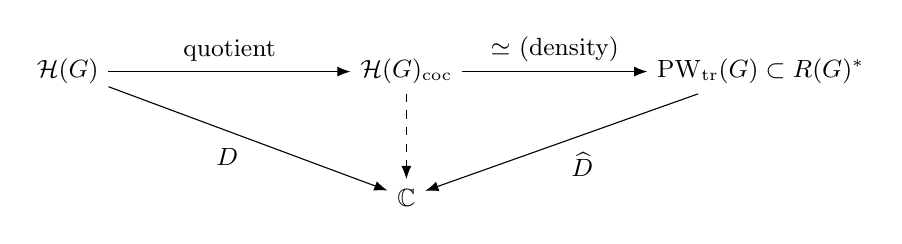
\begin{tikzpicture}[>=Latex,every node/.style={font=\small}]
\node (h) at (0,1.6) {$\calH(G)$};
\node (c) at (4.3,1.6) {$\calH(G)_{\rm coc}$};
\node (p) at (8.8,1.6) {$\PW_{\rm tr}(G)\subset R(G)^*$};
\node (k) at (4.3,0) {$\mathbb C$};
\draw[->] (h)--node[above]{quotient}(c);
\draw[->] (c)--node[above]{$\simeq$ (density)}(p);
\draw[->] (h)--node[below left]{$D$}(k);
\draw[->,dashed] (c)--(k);
\draw[->] (p)--node[below right]{$\widehat D$}(k);
\end{tikzpicture}
\caption{An invariant distribution $D$ factors through the cocenter (Lemma \ref{lem:conj}) and then through the trace image (Theorem \ref{thm:density}). Every linear functional $\widehat D$ on the trace image arises (Proposition \ref{prop:alg-dual}).}\label{fig:factorization}
\end{figure}
\begin{example*}
In the unramified block the trace image is $\mathbb C[u]\oplus\mathbb C^2$ (Proposition \ref{prop:algebraic-pw}). Choose any sequence of complex numbers $m_n$, for instance $m_n=n!$, and let $L$ be the functional with $L(z^n+z^{-n})=m_n$ that vanishes on the two exceptional coordinates. By Proposition \ref{prop:alg-dual} the functional $f\mapsto L(P_f)$, where $P_f$ is the trace polynomial of $f$, is an invariant distribution on $G$. No growth condition on the $m_n$ is required. Growth conditions appear only when one asks for an extension to a larger space of test functions.
\end{example*}

\subsection{What changes for the Schwartz space}\label{sec:schwartz}
This subsection indicates, without proofs, how the picture changes when $\calH(G)$ is replaced by the Schwartz space.

Recall from Subsection \ref{sec:schwartzbackground} that $\calC(G)=\varinjlim_J\calC(G/\!/J)$ is an inductive limit of Fr\'echet spaces, and that a tempered distribution is a linear functional that is continuous on each $\calC(G/\!/J)$. The Hecke algebra is dense in $\calC(G)$ and the inclusion is continuous. So a tempered distribution is determined by its restriction to $\calH(G)$, and the question is which distributions on $\calH(G)$ extend. For the Hecke algebra, continuity is automatic (Proposition \ref{prop:alg-dual}). For the Schwartz space, continuity is a substantive condition.

The natural Fourier transform on $\calC(G)$ is initially operator-valued on tempered representations; traces yield invariant spectral data. Only \emph{invariant} tempered distributions are candidates for factorization through the tempered \emph{trace} transform.

In spectral terms the condition for extension is a growth condition. On one family of unramified twists, with coordinate $z$, a functional $\lambda$ on trace polynomials is determined by its coefficients $c_n=\lambda(z^n)$. Three spaces of spectral test functions occur in this paper, and they have three different duals.
\begin{center}\small
\begin{tabularx}{\linewidth}{@{}p{.43\linewidth}X@{}}\toprule
Spectral test-function space & Condition on the dual coefficients $c_n$\\\midrule
Laurent polynomials, inductive-limit topology & None\\
Holomorphic functions on $\mathbb C^\times$, compact-open topology & $|c_n|\le CR^{|n|}$ for some $C$, $R$\\
Smooth functions on the unit circle & $|c_n|\le C(1+|n|)^N$ for some $C$, $N$\\\bottomrule
\end{tabularx}
\end{center}
These are three duality theories. They are compared in Theorem \ref{thm:three-duals}. The first row corresponds to $\calH(G)$ and the third to $\calC(G)$. The relation between them is one of the main themes of Sections \ref{sec:tempered-duality} and \ref{sec:admissible-duality}.

The detailed Plancherel and Schwartz Paley--Wiener descriptions must keep track of discrete-series summands, the smooth families on unitary unramified tori, and matching at the reducible points \cite{Cl91,Si79}.  A direct-product description with arbitrary independent values at the discrete-series points is not a valid substitute for these matching conditions. We do not state an independent exact Schwartz-image theorem here.

\begin{example}[Why invariance is necessary]
Fix $x_0\in G$ and let $T_{x_0}(f)=f(x_0)$. Point evaluation is continuous on $\calC(G)$, but it is not invariant for general $x_0$. Take $f,g$ such that $f^g\ne f$ and $f(x_0)\ne f^g(x_0)$. Then $\mathcal F_{\rm tr}(f-f^g)=0$ while $T_{x_0}(f-f^g)\ne0$. Thus no functional of the trace transform alone can recover this tempered distribution.
\end{example}

\section{Compatibility of the three trace Paley--Wiener theorems}\label{sec:pwcomparison}
The purpose of this section is to compare restriction of the spectrum with enlargement of the test-function space. We work with $G=\mathrm{SL}_2(F)$, where the residual characteristic is odd, and normalized induction $I(\chi)$ from the upper triangular Borel. All trace spaces below are vector spaces, not algebras under pointwise multiplication.

\subsection{The comparison maps}
Write $H=C_c^\infty(G)$ and $S=\mathcal C(G)$ for the Hecke and Harish-Chandra Schwartz algebras. For $X=\mathrm{ad},u,t$, let $R_X$ be the complex vector space freely generated by the corresponding irreducible admissible, unitarizable, or tempered representations. Trace additivity identifies $R_{\mathrm{ad}}$ with the complexified finite-length Grothendieck group. Put $T_X(f)(\pi)=\operatorname{tr}\pi(f)$, and write $E_X=T_X(H)$ and $E_S=T_t(S)$. In particular $E_t$ means compact-support tempered trace data, not the Schwartz image.

\begin{center}
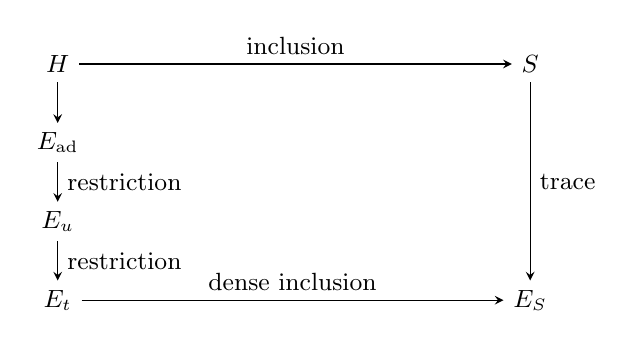
\begin{tikzpicture}[>=stealth, every node/.style={font=\small}]
\node (h) at (0,3) {$H$}; \node (s) at (6,3) {$S$};
\node (a) at (0,2) {$E_{\mathrm{ad}}$};
\node (u) at (0,1) {$E_u$};
\node (t) at (0,0) {$E_t$}; \node (e) at (6,0) {$E_S$};
\draw[->] (h)--node[above]{inclusion}(s);
\draw[->] (h)--(a); \draw[->] (a)--node[right]{restriction}(u);
\draw[->] (u)--node[right]{restriction}(t);
\draw[->] (s)--node[right]{trace}(e);
\draw[->] (t)--node[above]{dense inclusion}(e);
\end{tikzpicture}
\end{center}

\begin{theorem}\label{thm:pwcomparison}
The restriction maps $E_{\mathrm{ad}}\to E_u\to E_t$ are vector-space isomorphisms.
\end{theorem}
\begin{proof}
Surjectivity follows from the definitions. Suppose that $f\in H$ has zero trace on every irreducible tempered representation. Fix a smooth character $\xi$ of $\mathcal O_F^\times$ and put $\chi_{\xi,z}(\varpi^m a)=z^m\xi(a)$, where $z\in\mathbb C^\times$. The function
\[
P_{\xi,f}(z)=\operatorname{tr} I(\chi_{\xi,z})(f)
\]
is a Laurent polynomial by regularity of induced traces (the compact realization also gives this directly). For $|z|=1$ every constituent of the normalized induction is tempered. Additivity of traces gives $P_{\xi,f}(z)=0$ on the circle. Multiplying by a sufficiently large power of $z$ gives an ordinary polynomial with infinitely many roots, so $P_{\xi,f}$ vanishes identically.

The rank-one classification now gives vanishing on every irreducible principal series. The constituents at nontrivial quadratic inducing characters are already tempered. At the remaining reducibility point use $[I(|\cdot|)]=[\mathbf 1]+[\mathrm{St}]$. Since the Steinberg trace is zero, the trivial trace is zero as well. Supercuspidals are tempered because the center is finite. Thus every admissible irreducible trace vanishes, proving injectivity of both restrictions.
\end{proof}

By Kazhdan's density theorem \cite{Ka86}, the common kernel is the linear commutator span $[H,H]$. Consequently all three compact-support trace images identify with the algebraic cocenter $H/[H,H]$. This does not imply injectivity of the trace map on $H$ itself.

\subsection{Explicit coordinates and the unitary theorem}
Write $W$ for inversion on $\mathbb C^\times$, and $u=z+z^{-1}$. The good-functional trace Paley--Wiener theorem \cite{BDK86} requires uniform compact-open level and regularity on induced families. In rank one the only proper Levi is the diagonal torus. For a fixed principal-series block, regularity is exactly the Laurent-polynomial requirement on the total induced trace. The level condition is automatic for the proposed data in finitely many blocks: choose a principal congruence subgroup fixing the inducing compact model at that level and nonzero vectors in each exceptional constituent, and decrease it to accommodate the finitely many supercuspidals. For generic induced representations the fixed-vector dimension is independent of unramified twist. Thus the following coordinate descriptions follow from the classical classification and the good-functional theorem.

\begin{center}
\begin{tabular}{lll}
\hline
Block & $E_{\mathrm{ad}}\simeq E_u\simeq E_t$ & $E_S$ (see below)\\
\hline
Supercuspidal & $\mathbb C$ & $\mathbb C$\\
$\xi^2\ne1$ & $\mathbb C[z,z^{-1}]$ & $C^\infty(S^1)$\\
$\xi^2=1,\ \xi\ne1$ & $\mathbb C[u]\oplus\mathbb C^2$ & $C^\infty(S^1)^W\oplus\mathbb C^2$\\
$\xi=1$ & $\mathbb C[u]\oplus\mathbb C^2$ & $C^\infty(S^1)^W\oplus\mathbb C^2$\\
\hline
\end{tabular}
\end{center}
For $\xi^2\ne1$ choose one of the two inverse restrictions to units. For ramified quadratic $\xi$ the exceptional coordinates are the differences of the two constituent traces at each of $z=1,-1$. For $\xi=1$, use $d=\phi(\pi_+)-\phi(\pi_-)$ at $z=-1$ and $b=\phi(\mathrm{St})$. Set $c=q+q^{-1}$. The remaining traces are
\[
\phi(\pi_\pm)=\tfrac12(Q(-2)\pm d),\qquad
\phi(\mathbf 1)=Q(c)-b.
\]
Here $Q(u)$ is the total induced trace. In particular the same polynomial governs both the unitary principal series ($-2\le u\le2$) and complementary series ($2<u<c$). These conditions are necessary and sufficient within this block: extend the polynomial to the complex torus, impose the displayed sums at reducibility, and apply the good-functional theorem. This is an explicit unitary trace Paley--Wiener theorem, not an independent assumption.

\begin{example}
For $F=\mathbb Q_3$, take $Q(u)=u^2-2$, the Laurent polynomial $z^2+z^{-2}$. The total quadratic trace is $2$, and the trivial plus Steinberg trace is $82/9$. The individual traces depend on $d,b$. More generally $z^n+z^{-n}=2T_n(u/2)$, where $T_n$ is the Chebyshev polynomial.
\end{example}
\begin{center}
\begin{tikzpicture}[x=1.35cm,y=.38cm,>=stealth]
\draw[->] (-2.3,0)--(3.65,0) node[right]{$u$};
\draw[->] (0,-2.6)--(0,10) node[above]{$Q$};
\draw[teal,thick,domain=-2:2,samples=60] plot (\x,{\x*\x-2});
\draw[orange!80!black,thick,domain=2:3.333,samples=60] plot (\x,{\x*\x-2});
\foreach \x/\l in {-2/-2,2/2,3.333/{10/3}} {\draw (\x,.15)--(\x,-.15) node[below]{$\l$};}
\node[teal] at (-1.5,5) {tempered};
\node[orange!80!black] at (2.6,7) {complementary};
\end{tikzpicture}
\end{center}

\subsection{The Schwartz comparison and completion}
Arthur's trace Paley--Wiener theorem for Schwartz functions \cite[p.~174]{Ar94} gives a continuous open surjection onto smooth data on virtual tempered character parameter spaces. The rank-one coordinate model in the last column above uses the induced unitary circle, the independent difference of quadratic constituents at each reducibility point, and the independent Steinberg trace. In particular the unramified comparison is $(Q,d,b)\mapsto(Q|_{[-2,2]},d,b)$. The Steinberg representation is discrete series and contributes its own coordinate, not a value on the circle. The precise identification with Arthur's topology, including the normalization of virtual characters and global level filtration, is a remaining source-verification task (Remark 2026.1). The following density conclusion does not require that explicit identification.

\begin{theorem}\label{thm:pwcompletion}
The compact-support trace image $E_t$ is dense in $E_S$ with Arthur's quotient topology.
\end{theorem}
\begin{proof}
Compactly supported smooth functions are dense in $S$: on a fixed compact-open bi-invariant Schwartz stage, truncate on compact unions of double cosets with length bounded by $m$. The error in each weighted supremum seminorm tends to zero, by using a seminorm with one additional power of the length. Continuity and surjectivity of Arthur's trace map now give density.
\end{proof}
If the blockwise Fréchet models and their locally convex direct sum are identified with the Schwartz image, its completeness follows from completeness of those spaces. In that topology the completion of $E_t$ is $E_S$. This last global identification is recorded separately rather than assumed. On each proposed block, Fourier partial sums prove density in every smooth seminorm. Weyl averaging preserves convergence and exceptional coordinates may be held fixed.

\begin{center}
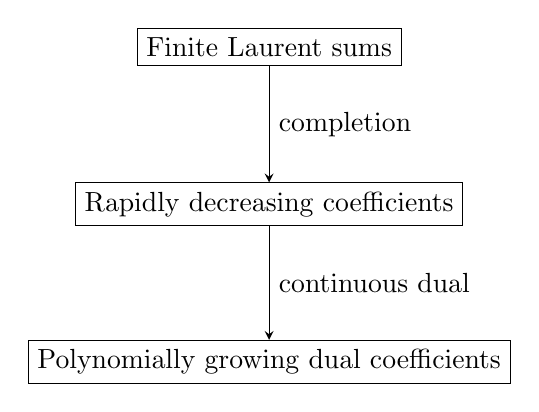
\begin{tikzpicture}[>=stealth]
\node[draw] (p) at (0,2) {Finite Laurent sums};
\node[draw] (s) at (0,0) {Rapidly decreasing coefficients};
\node[draw] (d) at (0,-2) {Polynomially growing dual coefficients};
\draw[->] (p)--node[right]{completion}(s);
\draw[->] (s)--node[right]{continuous dual}(d);
\end{tikzpicture}
\end{center}

\subsection{Instability of algebraic continuation}
Uniqueness of continuation must not be confused with continuity. The following elementary spectral calculation applies to the proposed smooth block model.
\begin{theorem}\label{thm:pwinstability}
For $s_0>0$, put $P_n(z)=q^{-ns_0}(z^n+z^{-n})$. Then $P_n|_{S^1}\to0$ in $C^\infty(S^1)$, but $P_n(q^{-s_0})\to1$.
\end{theorem}
\begin{proof}
The $k$th angular derivative has supremum at most $2n^kq^{-ns_0}$, which tends to zero for each $k$. At $q^{-s_0}$ the value is $1+q^{-2ns_0}$.
\end{proof}
Take $0<s_0<1$ for a complementary-series trace, or $s_0=1$ with $b=0$ for the trivial trace. Set the other exceptional coordinate to zero. By the admissible trace theorem these data have Hecke-algebra preimages. Consequently non-tempered evaluation is discontinuous for the smooth spectral topology. Its interpretation in Arthur's topology uses the identification in Remark 2026.1. This separates algebraic determination by tempered traces from continuous determination after completion.

\begin{center}
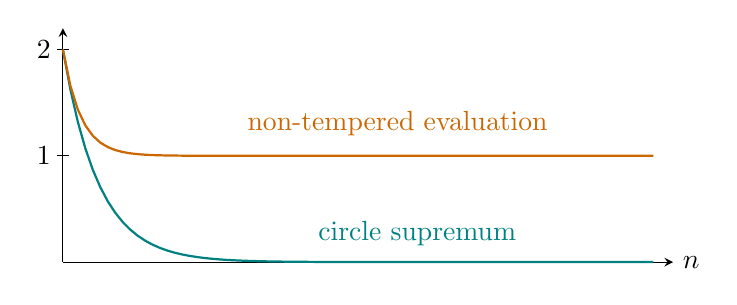
\begin{tikzpicture}[x=.25cm,y=1.35cm,>=stealth]
\draw[->] (0,0)--(31,0) node[right]{$n$};
\draw[->] (0,0)--(0,2.2);
\foreach \y in {1,2} {\draw (-.3,\y)--(.3,\y) node[left,xshift=-3pt]{$\y$};}
\draw[teal,thick,domain=0:30,samples=80] plot (\x,{2*3^(-\x/2)});
\draw[orange!80!black,thick,domain=0:30,samples=80] plot (\x,{1+3^(-\x)});
\node[teal] at (18,.27) {circle supremum};
\node[orange!80!black] at (17,1.3) {non-tempered evaluation};
\end{tikzpicture}
\end{center}

\subsection{Intermediate analytic spaces}
For $r>1$ put $A_r=\{z:r^{-1}<|z|<r\}$. The compact-open topology on $\mathcal O(A_r)^W$ makes evaluation at $q^{-s}$ continuous for $q^s<r$. Laurent polynomials are dense by Laurent expansion on compact subannuli. Cauchy's estimates give exponential decay of the Laurent coefficients at every rate strictly below $r$. For holomorphic functions on $\mathbb C^\times$ this holds at every finite rate. For smooth circle functions it is replaced by rapid polynomial decay. The exceptional coordinates can be appended as independent finite-dimensional summands; a non-tempered constituent trace only extends if the corresponding evaluation is continuous.

\begin{center}
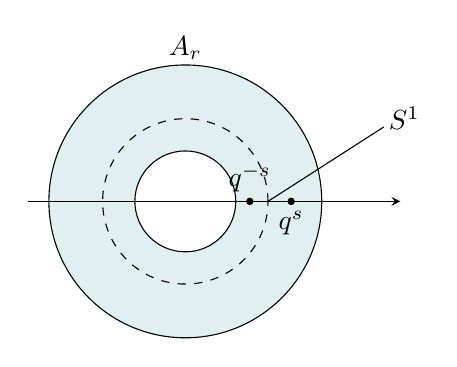
\begin{tikzpicture}[>=stealth,scale=1.05]
\fill[teal!12,even odd rule] (0,0) circle (1.65) (0,0) circle (.61);
\draw (0,0) circle (1.65); \draw (0,0) circle (.61);
\draw[dashed] (0,0) circle (1);
\draw[->] (-1.9,0)--(2.6,0);
\fill (.78,0) circle (.045) node[above]{$q^{-s}$};
\fill (1.28,0) circle (.045) node[below]{$q^s$};
\node at (0,1.85) {$A_r$};
\node at (2.65,1) {$S^1$};
\draw (1,0)--(2.4,.9);
\end{tikzpicture}
\end{center}
A research question is whether the trace images of Harish-Chandra $L^p$-Schwartz spaces, $0<p<2$, with decay controlled by $\Xi^{2/p}$ and all polynomial length weights, admit descriptions on such annuli with boundary regularity. Neither a radius formula nor surjectivity is asserted here.

\subsection{Duality and invariant distributions}
On the unramified polynomial summand use $B_0=1$, $B_n=z^n+z^{-n}$ for $n\ge1$. The locally convex inductive limit of bounded-degree polynomial spaces has every linear functional continuous. The inherited smooth topology is strictly weaker.
\begin{theorem}\label{thm:pwdual}
A functional $\ell$ on $\mathbb C[u]\oplus\mathbb C^2$ extends continuously to $C^\infty(S^1)^W\oplus\mathbb C^2$ if and only if $|\ell(B_n,0,0)|\le C(1+n)^N$ for all $n\ge0$ and some $C,N$.
\end{theorem}
\begin{proof}
Continuity bounds $\ell$ by finitely many smooth seminorms, and the $k$th derivatives of $B_n$ have supremum at most $2n^k$ for $n\ge1$. Conversely the coefficients in $h=a_0+\sum_{n\ge1}a_nB_n$ decrease rapidly, so the sum $\sum a_n\ell(B_n,0,0)$ converges absolutely and is bounded by a smooth seminorm by integration by parts. Append the two finite-dimensional functionals. Density proves uniqueness.
\end{proof}
The constant mode is independent and must be retained. Evaluation at $1$ has coefficients $2$ for $n\ge1$, evaluation at $-1$ has $2(-1)^n$, and the second angular derivative at $1$ has $-2n^2$. Complementary-series evaluation grows as $q^{ns}+q^{-ns}$ and fails the criterion. The trivial character similarly fails, whereas the independent Steinberg coordinate satisfies it.

Globally the anticipated topology is the locally convex direct sum of the block spaces, not their product. Its continuous dual is the product of the block duals. Bernstein finiteness at fixed compact-open level and the converse control of block stages must be checked in the Schwartz setting. No uniform growth estimate across all blocks is required if the direct-sum topology holds.

\subsection{Cocenters and the remaining research program}
The algebraic cocenter is $HH_0(H)$. The natural topological counterpart is $S/\overline{[S,S]}$. Identifying this with the Schwartz trace image requires the equality of its trace kernel with the closed commutator span; the trace theorem alone does not assert that equality. This modern interpretation motivates the comparison with Solleveld's work on Hochschild homology of reductive $p$-adic group algebras.
\begin{center}
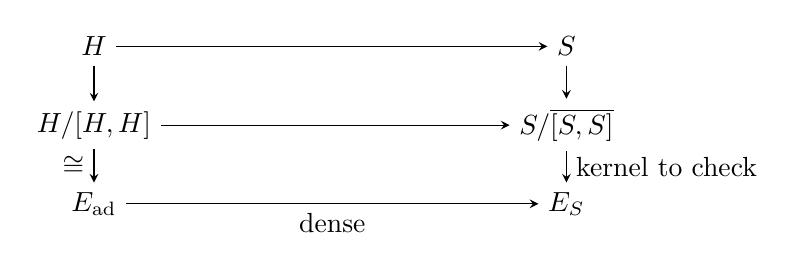
\begin{tikzpicture}[>=stealth]
\node (h) at (0,2) {$H$}; \node (s) at (6,2) {$S$};
\node (c) at (0,1) {$H/[H,H]$};
\node (d) at (6,1) {$S/\overline{[S,S]}$};
\node (a) at (0,0) {$E_{\mathrm{ad}}$}; \node (b) at (6,0) {$E_S$};
\draw[->] (h)--(s); \draw[->] (h)--(c); \draw[->] (s)--(d);
\draw[->] (c)--(d); \draw[->] (c)--node[left]{$\cong$}(a);
\draw[->] (d)--node[right]{kernel to check}(b);
\draw[->] (a)--node[below]{dense}(b);
\end{tikzpicture}
\end{center}
The priorities are to verify Arthur's virtual-character normalization and topology in rank one, identify the global completion and closed commutator kernel, and investigate intermediate holomorphic trace spaces. The algebraic comparison and elementary spectral estimates above are proved subject to their stated classical inputs; novelty relative to the literature is not claimed.

\section{Linear functionals on the tempered Paley--Wiener space}\label{sec:tempered-duality}
We now use the spectral coordinates of the preceding sections to describe invariant distributions. We distinguish the algebraic trace image from its smooth completion. All assertions about group distributions through a smooth block model use the corresponding topological trace theorem, not merely an algebraic parametrization.

\subsection{Sequence spaces and the constant mode}
Let $B_0=1$ and $B_n=z^n+z^{-n}$ for $n\ge1$. The variable $u=z+z^{-1}$ identifies the invariant Laurent polynomials with $\mathbb C[u]$. A smooth inversion-invariant circle function has a unique expansion $h=a_0+\sum_{n\ge1}a_nB_n$ with rapidly decreasing coefficients. Integration by parts in the angular variable gives rapid decay; conversely termwise differentiation of a rapidly decreasing series converges uniformly at every order. The constant coefficient $a_0$ is independent of the other coefficients and must not be omitted.

Let $s$ be the space of sequences with all seminorms $\sup_n(1+n)^k|a_n|$ finite, and let $\varphi$ be the finite sequences with the locally convex inductive-limit topology of their finite-dimensional coordinate spaces. The Fourier expansion identifies $C^\infty(S^1)^W$ topologically with $s$. The polynomial space is identified with $\varphi$. In the unramified block the smooth space is modeled by $s\oplus\mathbb C^2$, with coordinates $(h,d,b)$; $d$ is the quadratic constituent difference and $b$ is the Steinberg trace. The representation-theoretic identification of this model is discussed in Section~\ref{sec:pwcomparison}.

\begin{theorem}\label{thm:duality-moments}
A linear functional on $\varphi\oplus\mathbb C^2$ extends continuously to $s\oplus\mathbb C^2$ if and only if its moments $m_n=\lambda(B_n,0,0)$ satisfy $|m_n|\le C(1+n)^N$ for some $C,N$. The extension is unique, and its two exceptional coefficients are unrestricted.
\end{theorem}
\begin{proof}
Continuity bounds the functional by finitely many seminorms. Applying this bound to the coordinate vectors gives the necessary estimate. Conversely $\sum a_nm_n$ converges absolutely and is bounded by $C\sup_n(1+n)^{N+2}|a_n|\sum_n(1+n)^{-2}$. Add the two ordinary scalar functionals. Finite sequences are dense in $s$, proving uniqueness.
\end{proof}
For example, second angular differentiation at $z=1$ has moments $-2n^2$ for $n\ge1$ and zero constant moment. It is tempered in the spectral model. The generic ramified blocks use bilateral Laurent moments indexed by $\mathbb Z$; the proof is unchanged with $|n|$ in the weights. Ramified quadratic blocks use the same even sequence space and two independent constituent-difference coordinates.

\subsection{Reducibility as a split exact sequence}
Put $c=q+q^{-1}$. In the unramified algebraic block use ambient coordinates $(Q,x_+,x_-,t,b)$, where $t$ is the trivial trace. Define
\[
D(Q,x_+,x_-,t,b)=(x_++x_--Q(-2),\,t+b-Q(c)).
\]
The algebraic trace space is $\ker D$ by the good-functional theorem. The map has a continuous right inverse $(v,w)\mapsto(0,v,0,w,0)$ for the polynomial inductive-limit topology. Thus the sequence is split and its continuous dual is exact:
\[
0\longrightarrow(\mathbb C^2)'\xrightarrow{D'} A'
 \longrightarrow(\ker D)'\longrightarrow0,\qquad
 A=\mathbb C[u]\oplus\mathbb C^4.
\]
The image of $D'$ is generated by
$(-\operatorname{ev}_{-2},1,1,0,0)$ and
$(-\operatorname{ev}_c,0,0,1,1)$.
The same construction works in holomorphic spaces where both evaluations are continuous. In the tempered space the second relation must instead be removed along with the trivial coordinate: evaluation at $c$ is not defined continuously on smooth circle functions. There remains one constraint, $x_++x_-=h(-1)$, and an independent Steinberg coordinate. For a ramified quadratic block both sum constraints are circle evaluations and are continuous.

\begin{center}
\begin{tikzpicture}[>=stealth]
\node (e) at (0,1.5) {$E$};\node (a) at (3.5,1.5) {$A$};\node (c) at (7,1.5) {$\mathbb C^2$};
\node (ed) at (0,0) {$E'$};\node (ad) at (3.5,0) {$A'$};\node (cd) at (7,0) {$(\mathbb C^2)'$};
\draw[->] (e)--(a);\draw[->] (a)--node[above]{$D$}(c);
\draw[->] (cd)--node[below]{$D'$}(ad);\draw[->] (ad)--(ed);
\foreach \x/\y in {e/ed,a/ad,c/cd}{\draw[dashed,->] (\x)--(\y);}
\end{tikzpicture}
\end{center}
Solving the algebraic constraints gives $x_\pm=(Q(-2)\pm d)/2$ and $t=Q(c)-b$. Every spectral functional has a unique normal form
\[
\lambda(Q,d,b)=\sum_{n\ge0}a_nm_n+\alpha d+\beta b.
\]
For polynomials the sum is finite; in the smooth model it converges by Theorem~\ref{thm:duality-moments}. In particular the nonzero quadratic difference and Steinberg character both have zero Laurent moments. The exceptional coordinates are essential for uniqueness.

\subsection{Invariant distributions and global topology}
Let $H=C_c^\infty(G)$ and $S=\mathcal C(G)$. Conjugation invariance on $H$ is equivalent to vanishing on convolution commutators. Indeed a conjugation-invariant functional has equal values on $f*g$ and $g*f$ by integrating translates, and conversely a compact-open approximate identity expresses conjugation differences as commutators. For the latter, choose a compact-open subgroup fixing $f$ on both sides, write the conjugation difference as the commutator of a translated idempotent and a translated $f$, and use convolution associativity. The same equivalence holds for continuous functionals on $S$ by density of $H$ and continuity of multiplication and conjugation. Kazhdan density identifies the algebraic cocenter with the algebraic trace image. All linear forms on $H$ are continuous for its locally convex inductive limit of finite-dimensional support-and-level stages.

For Schwartz functions the required identity is $\ker T_t=\overline{[S,S]}$. Arthur's open trace theorem \cite[p.~174]{Ar94} identifies the quotient by its trace kernel topologically with the smooth trace image. Solleveld's survey on group algebras, Examples 5.10 and 5.12 and Theorem 5.14, is a source for the closed-commutator identification; its exact version and hypotheses must be reconciled with Arthur's topology. Until that verification is complete, the assertion that every invariant tempered distribution has the displayed normal form is conditional on this identification.

\begin{proposition}\label{prop:duality-global}
For a locally convex direct sum $E=\bigoplus_{\mathfrak s}E_{\mathfrak s}$, restriction identifies $E'$ with $\prod_{\mathfrak s}E_{\mathfrak s}'$.
\end{proposition}
\begin{proof}
A functional on the sum is continuous precisely when all restrictions are continuous, by the defining final locally convex topology. The inverse sends a family of functionals to the finite sum of their values on each test vector.
\end{proof}
\begin{center}
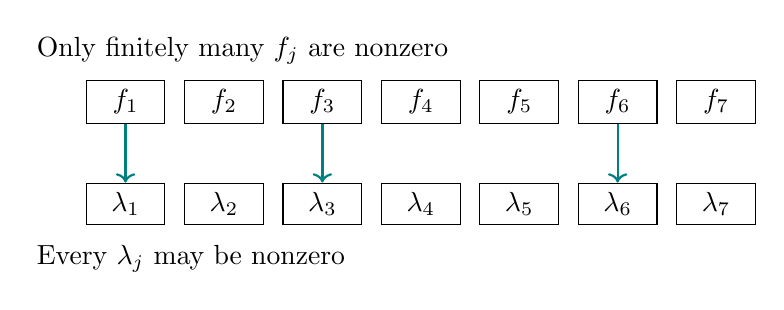
\begin{tikzpicture}
\foreach \n in {1,...,7}{
\node[draw,minimum width=1cm] (a\n) at (\n*1.25,1) {$f_{\n}$};
\node[draw,minimum width=1cm] (b\n) at (\n*1.25,-.3) {$\lambda_{\n}$};}
\foreach \n in {1,3,6}{\draw[teal,thick,->] (a\n)--(b\n);}
\node[anchor=west] at (0,1.65) {Only finitely many $f_j$ are nonzero};
\node[anchor=west] at (0,-1) {Every $\lambda_j$ may be nonzero};
\end{tikzpicture}
\end{center}
In the anticipated global Schwartz model the growth constants and exponents may depend on the block; a single uniform exponent is not required. To identify the topology, use the stages $S^{K_m\times K_m}$ for principal congruence subgroups $K_m$. Bernstein finiteness restricts each stage to finitely many blocks. The converse requires realization of the full smooth block trace image at sufficiently deep fixed level with continuous control of seminorms. Types and blockwise Morita equivalences are useful tools. See Solleveld, \emph{On completions of Hecke algebras}, arXiv:1612.01776, for a direction to investigate.

\subsection{Topologies on distribution spaces}
The weak dual topology is pointwise convergence on test vectors. The strong dual topology is uniform convergence on bounded subsets, and the compact-convergence topology is uniform convergence on compact subsets. On $\varphi'$ the strong dual topology is the ordinary product topology of all sequences, since bounded subsets of $\varphi$ lie in finite-dimensional stages. For $s'$ the standard strong dual sequence-space model is the inductive limit of weighted bounded sequence spaces with norms $\sup_n |m_n|/(1+n)^N$. In particular a family of tempered spectral functionals is equicontinuous exactly when it satisfies a common polynomial estimate. These facts distinguish individual growth from uniform estimates on families.

\section{Linear functionals on the admissible Paley--Wiener space}\label{sec:admissible-duality}
The admissible trace image is algebraic, but different completions of its polynomial coordinates provide intermediate dual spaces. We develop the Laurent criterion and then examine the action of the Bernstein center. The holomorphic models are spectral constructions; their identification with any independently defined notion of analytic distributions on $G$ is not assumed.

\subsection{The unified Laurent criterion}
For $r>1$ let $A_r=\{r^{-1}<|z|<r\}$. Append the same two exceptional scalar coordinates to each of the spaces below. Restriction gives dense continuous inclusions
\[
\mathbb C[z,z^{-1}]^W\ \longrightarrow\
\mathcal O(\mathbb C^\times)^W\ \longrightarrow\
\mathcal O(A_r)^W\ \longrightarrow\ C^\infty(S^1)^W.
\]
The holomorphic spaces have the compact-open topology. Density follows by Laurent truncation, or Fourier truncation on the circle. The continuous dual arrows reverse direction.
\begin{center}
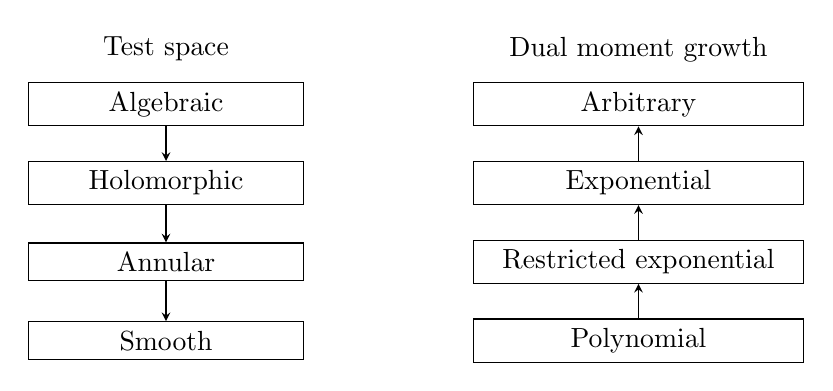
\begin{tikzpicture}[>=stealth]
\foreach \y/\a/\b in {3/Algebraic/Arbitrary,2/Holomorphic/Exponential,1/Annular/Restricted exponential,0/Smooth/Polynomial}{
\node[draw,minimum width=3.5cm] (l\y) at (0,\y) {\a};
\node[draw,minimum width=4.2cm] (r\y) at (6,\y) {\b};}
\foreach \i/\j in {3/2,2/1,1/0}{\draw[->] (l\i)--(l\j);\draw[->] (r\j)--(r\i);}
\node at (0,3.7) {Test space};\node at (6,3.7) {Dual moment growth};
\end{tikzpicture}
\end{center}
\begin{theorem}\label{thm:duality-holomorphic}
A linear functional with moments $m_n$ on the invariant Laurent polynomial space is continuous for the algebraic inductive limit without restriction. It extends continuously to $\mathcal O(\mathbb C^\times)^W$ precisely when $|m_n|\le CR^n$ for some $R>1$, and to $\mathcal O(A_r)^W$ precisely when such a bound holds with $1<R<r$. The smooth extension criterion is Theorem~\ref{thm:duality-moments}. Continuous extension to $C(S^1)^W$ holds precisely when the moments are the integrals of $B_n$ against a finite inversion-invariant complex measure.
\end{theorem}
\begin{proof}
For the holomorphic spaces put $p_R(h)=\sup_{R^{-1}\le|z|\le R}|h(z)|$, with $R<r$ in the annular case. A continuous functional is bounded by a single such seminorm up to a constant. Since $p_R(B_n)\le2R^n$, necessity follows. Conversely choose $R'>R$ within the allowed range. Cauchy's coefficient estimate yields $|a_n|\le p_{R'}(h)(R')^{-n}$. The defining moment sum converges absolutely and is bounded by a constant times $p_{R'}(h)\sum_{n\ge0}(R/R')^n$. Density proves uniqueness. For continuous circle functions, extend by composing with inversion averaging and apply the Riesz representation theorem; symmetrize the resulting finite complex measure. Conversely integration against such a measure is bounded for the uniform norm.
\end{proof}

\subsection{Growth radii and examples}
Define $\rho(\lambda)=\limsup_{n\to\infty}|m_n|^{1/n}$. The entire punctured-plane extension is equivalent to $\rho<\infty$, and the annular extension is equivalent to $\rho<r$. Tempered extension is strictly stronger than $\rho\le1$. For example $m_n=\exp(\sqrt n)$ has radius one and extends to every open annulus but fails every polynomial bound. The algebraic trace theorem realizes any moment sequence as an invariant distribution by pullback, including $m_n=n!$ which has no holomorphic extension.
\begin{center}\small
\begin{tabular}{lll}
\hline
Moments ($n\ge1$)& Radius & Tempered extension\\\hline
$1,\ n^3$ & $1$ & yes\\
$\exp(\sqrt n)$ & $1$ & no\\
$2^n$ & $2$ & no\\
$q^{sn}+q^{-sn}$ ($s>0$) & $q^s$ & no\\
$n!,\ \exp(n^2)$ & $\infty$ & no\\\hline
\end{tabular}
\end{center}
\begin{center}
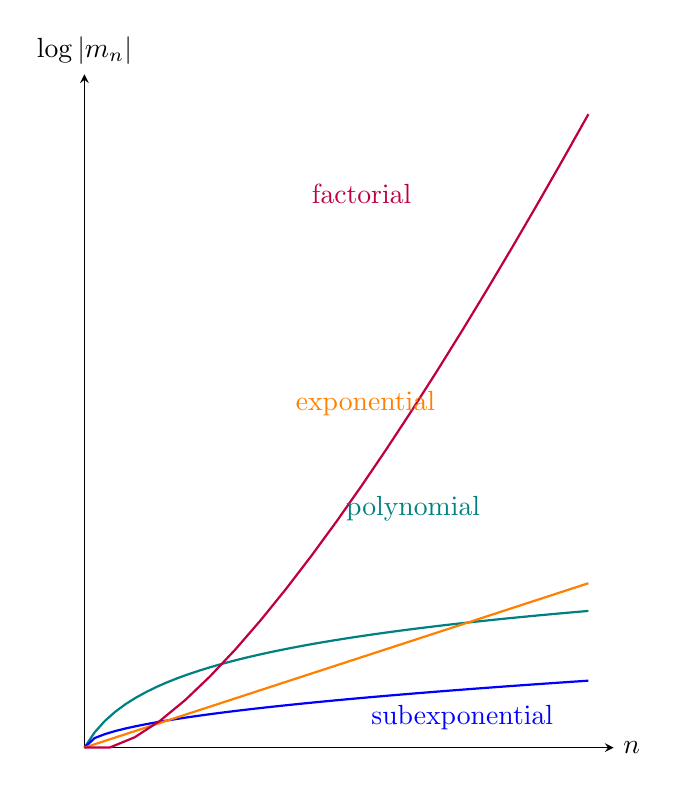
\begin{tikzpicture}[x=.32cm,y=.19cm,>=stealth]
\draw[->] (0,0)--(21,0) node[right]{$n$};
\draw[->] (0,0)--(0,45) node[above]{$\log |m_n|$};
\draw[teal,thick,domain=0:20,samples=50] plot (\x,{3*ln(\x+1)});
\draw[blue,thick,domain=0:20,samples=50] plot (\x,{sqrt(\x)});
\draw[orange,thick,domain=0:20] plot (\x,{\x*ln(3)/2});
\draw[purple,thick] plot coordinates {(0,0)(1,0)(2,.693)(3,1.792)(4,3.178)(5,4.787)(6,6.579)(7,8.525)(8,10.605)(9,12.802)(10,15.104)(11,17.502)(12,19.987)(13,22.552)(14,25.191)(15,27.899)(16,30.672)(17,33.505)(18,36.395)(19,39.340)(20,42.336)};
\node[teal,anchor=west] at (10,16) {polynomial};
\node[blue,anchor=west] at (11,2) {subexponential};
\node[orange,anchor=west] at (8,23) {exponential};
\node[purple] at (11,37) {factorial};
\end{tikzpicture}
\end{center}
The principal-series trace is evaluation of $Q$ at $z+z^{-1}$. The quadratic characters are $(Q(-2)\pm d)/2$, the Steinberg character is $b$, and the trivial character is $Q(c)-b$. Complementary-series evaluation at $z=q^{-s}$ has moments $q^{sn}+q^{-sn}$ and $\rho=q^s$, so $s=\log\rho/\log q$. Trivial evaluation has radius $q$ and extends to $A_r$ exactly for $r>q$. Pure exceptional functionals have all moments zero, including the constant moment. Their growth radius is zero regardless of their nonzero exceptional coefficients.

\subsection{The Bernstein center and a discrete recurrence}
The unramified Bernstein center $\mathbb C[u]$ acts by
\[
p\cdot(Q,d,b)=(pQ,p(-2)d,p(c)b).
\]
On the dual use $(p\lambda)(f)=\lambda(pf)$. For $n\ge2$, $uB_n=B_{n+1}+B_{n-1}$, while $uB_0=B_1$ and $uB_1=B_2+2B_0$.
\begin{theorem}\label{thm:duality-eigen}
If $u\lambda=\mu\lambda$, then
\[
m_1=\mu m_0,\quad m_2+2m_0=\mu m_1,\quad
m_{n+1}+m_{n-1}=\mu m_n\quad(n\ge2).
\]
Writing $\mu=z_0+z_0^{-1}$, the unique solution is $m_n=m_0(z_0^n+z_0^{-n})$ for $n\ge1$. The exceptional coefficients satisfy $(-2-\mu)\alpha=(c-\mu)\beta=0$.
\end{theorem}
\begin{proof}
Apply the eigen-equation to the polynomial basis and to the two exceptional coordinate vectors. The displayed evaluation sequence satisfies all initial conditions and the recurrence, which determines it uniquely.
\end{proof}
Thus the central eigenspace has dimension one except at $-2,c$, where it has dimension two. This recovers the exceptional support fibers through duality.
\begin{center}
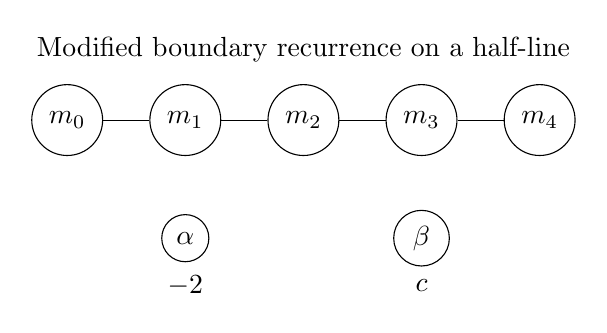
\begin{tikzpicture}
\foreach \n in {0,...,4}{\node[circle,draw,minimum size=9mm] (v\n) at (1.5*\n,0) {$m_{\n}$};}
\foreach \n/\m in {0/1,1/2,2/3,3/4}{\draw (v\n)--(v\m);}
\node at (3,.9) {Modified boundary recurrence on a half-line};
\node[circle,draw] at (1.5,-1.5) {$\alpha$};
\node[circle,draw] at (4.5,-1.5) {$\beta$};
\node at (1.5,-2.1) {$-2$};\node at (4.5,-2.1) {$c$};
\end{tikzpicture}
\end{center}
This is a tridiagonal sequence model, not the literal Bruhat--Tits adjacency operator. Comparison with the radial Satake operator is a possible further direction.

\subsection{Generalized central eigendistributions}
\begin{theorem}\label{thm:duality-jets}
For $m\ge1$, the space of functionals satisfying $(u-\mu)^m\lambda=0$ has dimension
$m+\mathbf1_{\{\mu=-2\}}+\mathbf1_{\{\mu=c\}}$. Its polynomial part consists of the evaluation jets $Q\mapsto Q^{(j)}(\mu)$ for $0\le j<m$.
\end{theorem}
\begin{proof}
The polynomial functional factors through $\mathbb C[u]/(u-\mu)^m$. Taylor expansion gives the stated basis of the dual of this quotient. Each exceptional summand is one-dimensional and is annihilated by $(u-\mu)^m$ exactly at its central character.
\end{proof}
For $\mu\in[-2,2]$, Markov's inequality for polynomial derivatives on a compact interval gives polynomial growth of the jet moments, since $B_n=2T_n(u/2)$ has degree $n$ and supremum two there. In particular $B_n'(2)=n^2$. For $\mu\notin[-2,2]$, choose the root $z_0$ of $z+z^{-1}=\mu$ with $|z_0|>1$. It varies holomorphically locally with $\mu$ and has nonzero logarithmic derivative. A nonzero linear combination of jets of highest order $j$ has leading moment $z_0^n$ times a polynomial of degree $j$ with nonzero leading coefficient, plus an exponentially decreasing term times a polynomial. It cannot be polynomially bounded. At $\mu=c$ the independent Steinberg functional remains tempered even though the polynomial jets do not. Thus the central character alone does not decide temperedness.

\subsection{Generating functions and central finiteness}
Define the formal series $F_\lambda(w)=\sum_{n\ge0}m_nw^n$. Its analytic radius is $1/\rho$ by Cauchy--Hadamard, with the usual zero and infinity conventions. For evaluation at $\mu$,
\[
F_\lambda(w)=\frac{1-w^2}{1-\mu w+w^2}.
\]
Evaluation at $2$ gives $(1+w)/(1-w)$ and evaluation at $-2$ gives $(1-w)/(1+w)$. Jets give derivatives of the rational expression. Pure exceptional functionals give zero.
\begin{proposition}\label{prop:duality-rational}
Central finiteness (finite-dimensional span of $\mathbb C[u]\lambda$) implies rationality of $F_\lambda$, but the converse is false in general.
\end{proposition}
\begin{proof}
A finite-dimensional central module is annihilated by a nonzero polynomial. Factoring that polynomial and using the Chinese remainder theorem expresses the polynomial functional as a finite sum of jets. Their generating functions are rational. For the converse counterexample, take $m_0=0$, $m_1=1$, and $m_n=0$ for $n\ge2$. Then $F_\lambda(w)=w$ is rational. The functional is proportional to extraction of the coefficient of $z$ from an invariant Laurent polynomial. No nonzero $p(u)$ annihilates it: the bilinear constant-coefficient pairing on symmetric Laurent polynomials is nondegenerate, since the basis $B_n$ is orthogonal with nonzero diagonal values. The functional equals constant-coefficient pairing with $B_1/2$, so annihilation would force $p(u)B_1=0$, impossible in the Laurent polynomial domain.
\end{proof}
The exact replacement criterion is rationality of the monomial moment series $M_\lambda(t)=\sum_{n\ge0}\lambda(u^n,0,0)t^n$. An eventual recurrence of its coefficients produces an annihilating polynomial after multiplying by a sufficiently large power of $u$; conversely an annihilating polynomial yields a recurrence. Exceptional summands can be killed by multiplying by $(u+2)(u-c)$. The formal identity
\[
F_\lambda(w)=\frac{1-w^2}{1+w^2}
M_\lambda\left(\frac{w}{1+w^2}\right)
\]
explains why rationality of $M_\lambda$ implies rationality of $F_\lambda$ but not conversely. The distinction matters for any comparison with quasi-finiteness in Section~\ref{sec:descent}.

\subsection{Exceptional modes and further questions}
The subspace with zero polynomial moments in the chosen unramified splitting is spanned by the quadratic character difference and the Steinberg character. In ramified quadratic blocks it is spanned by the two constituent differences. All are tempered. The subspace depends on the splitting: with the algebraic difference coordinate of Subsection~\ref{subsec:pw-coordinates} in place of the Steinberg trace it is a different subspace. Theorems~\ref{thm:twosplit} and~\ref{thm:exact} give the intrinsic description by weak constant terms and compare the two splittings; literal elliptic support is a different notion. The remaining tasks are to identify the global smooth topology and its cocenter, compare analytic spectral functionals with group-side decay or analyticity, and compare central finiteness with the original quasi-finiteness definition. None of these identifications is inferred solely from the elementary moment calculations.


\section{Admissible invariant distributions: local regularity, descent, and spectral finiteness}\label{sec:descent}
The preceding sections distinguish algebraic spectral data from their topological completions. We now ask what such data imply locally on the group. The important point is that the size of the Laurent moments at infinity need not govern singular behavior on compact subsets. We continue to assume that $F$ is a $p$-adic field of odd residual characteristic.

\subsection{Admissibility and local regularity}
For compact open subgroups $K'\subset K$ and an irreducible smooth representation $\sigma$ of $K'$, let
\[
e_\sigma(k)=\frac{\dim\sigma}{\operatorname{vol}(K')}
 \operatorname{tr}\sigma(k^{-1})\quad(k\in K'),
\]
extended by zero. With Haar measure on $G$ this is the central isotypic idempotent in the convolution algebra of $K'$. Say that $\sigma$ intertwines the trivial type on $K$ in $G$ if for some $g\in G$ its restriction to $K'\cap gKg^{-1}$ contains the trivial representation.

We use the local admissibility condition of the original notes: an invariant distribution $D$ is $(G,K)$-admissible at $\gamma$ if $D(f*e_\sigma)=0$ for all $f$ supported in $\gamma K$, all $K'\subset K$, and all $\sigma$ not intertwining the trivial type on $K$. In this formulation one may use the contragredient idempotent instead, with the corresponding change of type label. The intertwining condition with the trivial type is unchanged. Admissibility on an invariant open set means that such a $K$ exists at every point of the set.

The Harish-Chandra regularity input used below is that irreducible admissible characters satisfy the local condition, and admissible invariant distributions have locally integrable invariant representatives, locally constant on the regular semisimple set and with locally bounded discriminant-normalized density. See \cite{HC99} for the regularity theory; the precise hypotheses and formulation in that source require a source-level audit (Remark 2026.8). We use the condition at every point, not only at regular points.

\begin{lemma}\label{lem:admissibility-local}
The local admissibility condition is preserved by shrinking $K$, taking finite linear combinations of admissible distributions, and replacing a distribution by one agreeing with it on all test functions in an open neighborhood of $\gamma$.
\end{lemma}
\begin{proof}
If a type of a smaller subgroup intertwines the trivial representation on $K$, the same intertwining element works after $K$ is shrunk: the intersection on which invariance is required decreases. Thus failure to intertwine the smaller trivial type implies failure to intertwine the larger one. Also $\gamma K_1\subset\gamma K$ when $K_1\subset K$. This proves the first assertion. For finitely many distributions take a common smaller subgroup and use linearity. Finally choose $K$ with $\gamma K$ contained in the neighborhood of agreement. For $K'\subset K$, convolution on the right by $e_\sigma$ preserves the support condition in $\gamma K$. The defining test therefore takes the same value on both distributions.
\end{proof}

Representability by a locally integrable function, local constancy on the regular set, and a locally bounded normalized density are distinct from global temperedness. In particular, a point mass at the identity is invariant but is not represented by a locally integrable function. We will return to this example below.

\subsection{Local finite-character interpolation}
Let $\mathfrak s$ be a principal-series Bernstein component. Fix the restriction $\xi$ of an inducing character to $\mathcal O^\times$ and use $\chi_{\xi,z}(\varpi^m a)=z^m\xi(a)$. For a regular split element $a(t)$ with $t=\varpi^m a$, the total induced character is
\[
\Theta_{I(\chi_{\xi,z})}(a(t))=
\frac{\xi(a)z^m+\xi(a)^{-1}z^{-m}}{|t-t^{-1}|}.
\]
It is zero on the regular elliptic set. This is a formula for the full induced character even at reducible parameters.

\begin{lemma}\label{lem:compact-exponents}
For every compact subset $C$ of $G$, the integers $v(t)$ occurring among split eigenvalues of regular elements of $C$ form a bounded set.
\end{lemma}
\begin{proof}
The traces of matrices in $C$ are bounded in absolute value. If $|t|\ne1$, the ultrametric inequality gives $|t+t^{-1}|=\max(|t|,|t|^{-1})=q^{|v(t)|}$. If $|t|=1$, the valuation is zero. This gives a common bound.
\end{proof}

\begin{theorem}[Local finite-character interpolation]\label{thm:local-interpolation}
Assume the classical character formula and local integrability of irreducible characters. Let $L$ be an arbitrary algebraic linear functional on the Laurent-polynomial total-trace coordinate of a principal-series block (with Weyl invariance where appropriate). Define $D_L(f)=L(z\mapsto\operatorname{tr}I(\chi_{\xi,z})(f))$. On every relatively compact open set $V$ in $G$, this distribution is a finite linear combination of irreducible tempered character distributions. The combination may depend on $V$. Its regular invariant density is zero on the elliptic set, and on the split set equals
\[
F_L(a(t))=
\frac{\xi(a)L(z^m)+\xi(a)^{-1}L(z^{-m})}{|t-t^{-1}|}
\]
in a non-Weyl-invariant block. In a Weyl-invariant block the numerator is evaluated as a single invariant Laurent polynomial.
\end{theorem}
\begin{proof}
Put $C=\overline V$. By Lemma~\ref{lem:compact-exponents}, the numerators on $C$ lie in the finite-dimensional space of Laurent polynomials with exponents between $-M$ and $M$ for some $M$. In the self-inverse case intersect this space with the Weyl-invariant subspace. Call the resulting space $P_M$.

Evaluation at generic points of the unit circle spans $P_M^*$: otherwise a nonzero Laurent polynomial would vanish at every such point, contradicting the polynomial identity theorem. Choose a finite spanning set of evaluations at parameters $z_j$, avoiding the finitely many reducibility points, and constants $c_j$ with $L|_{P_M}=\sum_j c_j\operatorname{ev}_{z_j}$.

For $f$ supported in $V$, the induced trace polynomial belongs to $P_M$. To see this without assuming interchange with an infinite functional, first multiply the pointwise numerator by $f$ and integrate the finitely many coefficient functions. These coefficient functions are locally integrable on $C$: they are fixed linear combinations of the finitely many generic induced character functions, obtained from an injective evaluation matrix on $P_M$. The regular semisimple complement is Haar-null, so the character integral for each $z$ equals the integral of this finite expansion. This proves the asserted polynomial membership and the identity
\[
D_L(f)=\sum_j c_j\Theta_{I(\chi_{\xi,z_j})}(f).
\]
The parameters are unitary and irreducible, hence tempered. The same finite interpolation gives the displayed pointwise formula on the regular set in $V$. Exhaustion by relatively compact open sets gives a locally integrable representative on $G$; the representatives agree on overlaps up to null sets, and their regular formulas agree pointwise.
\end{proof}

For $\xi=1$, put $m_n=L(B_n)$, with $B_0=1$. The formula simplifies to
\[
F_L(a(t))=\frac{1}{|t-t^{-1}|}
\begin{cases}
m_{|v(t)|},&v(t)\ne0,\\
2m_0,&v(t)=0.
\end{cases}
\]
The constant mode is indispensable. On compact sets the normalized density is bounded, since only finitely many moments occur there.

\begin{theorem}[Finite Bernstein support]\label{thm:finite-block-admissibility}
Assume the algebraic block descriptions in Section~\ref{sec:pwcomparison} and the Harish-Chandra character admissibility input above. Every invariant distribution with finite Bernstein spectral support satisfies the local admissibility condition and is locally representable. No global bound on its Laurent moments is needed.
\end{theorem}
\begin{proof}
In a principal-series block, decompose its spectral functional into the continuous-family functional $L$ and the two exceptional coefficients when present. The latter are finite combinations of irreducible characters. Each supercuspidal block is a single character coordinate since $G$ has no nontrivial unramified characters. Theorem~\ref{thm:local-interpolation} represents the $L$ contribution locally as a finite sum of characters. There are finitely many blocks by hypothesis, so the total sum is finite on each relatively compact open set. Lemma~\ref{lem:admissibility-local} and character admissibility give the assertion. Local integrability and the normalized bound follow either from the finite character formula or from regularity.
\end{proof}
The theorem is conditional on the stated classical inputs, not a new assertion of a general regularity theorem. In particular it does not follow from finite Bernstein support of a multiplier merely by treating that multiplier as a finite spectral sum.

\begin{center}
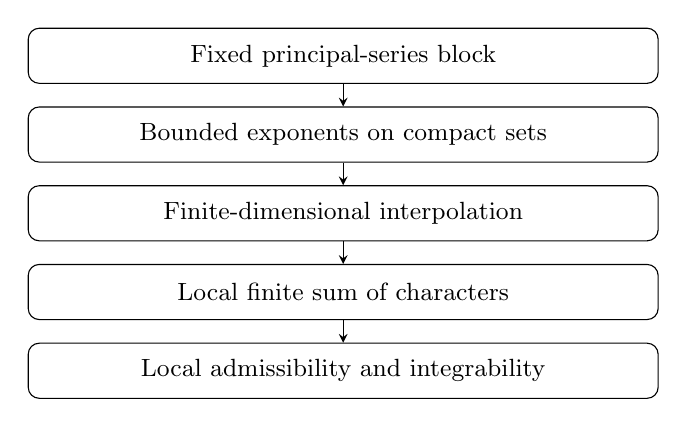
\begin{tikzpicture}[>=stealth,every node/.style={font=\small}]
\foreach \y/\t in {4/{Fixed principal-series block},3/{Bounded exponents on compact sets},2/{Finite-dimensional interpolation},1/{Local finite sum of characters},0/{Local admissibility and integrability}}{
\node[draw,rounded corners,minimum width=8cm,minimum height=7mm] (v\y) at (0,\y) {\t};}
\foreach \a/\b in {4/3,3/2,2/1,1/0}{\draw[->] (v\a)--(v\b);}
\end{tikzpicture}
\end{center}

\begin{example}
In the unramified block take $m_n=n!$ for $n\ge1$ and any $m_0$, with the exceptional coefficients zero. The theorem proves local admissibility, whereas the Laurent criterion rules out extension to the punctured-plane holomorphic spectral space and to the smooth circle spectral space. The example separates local regularity from global analytic and tempered growth. The same construction works with $m_n=\exp(n^2)$, while $m_n=\exp(\sqrt n)$ extends to every open annular spectral space but not the smooth circle. The group-side temperedness conclusions use the smooth trace identification in the preceding sections.
\end{example}

\subsection{Three kinds of descent}
For a locally integrable invariant density $F_D$ that is locally constant on the regular set, distinguish its ordinary restriction to a torus, its normalized split restriction
\[
h_D(a)=|\Delta_G(a)|^{1/2}F_D(a),
\]
and the normalized Jacquet-module or constant-term constructions. The first two are initially functions on the regular torus; the third is representation-theoretic and involves asymptotic character theory \cite{Ca93,Si79}. The Weyl integration formula expresses the split part of $D(f)$ as
\[
\frac12\int_A h_D(a)F_f^A(a)\,da
\]
with compatible measures and normalized orbital integral $F_f^A$. This identity does not establish that $h_D$ is locally constant at singular points or that it is a Jacquet-module character. A locally constant function on the abelian torus defines an admissible distribution for the local type condition: choose a unit subgroup on which the density is constant; convolution with a nontrivial character of any smaller subgroup vanishes. Conversely the local condition for a torus forces a locally constant density there, by the finite Fourier decomposition of locally constant test functions on the chosen compact open coset.

\begin{example}[Failure of a general descent theorem]\label{ex:descent}
For the trivial representation, the normalized split restriction is $|t-t^{-1}|$. For $t=1+x$ sufficiently close to one, $t-t^{-1}=x(2+x)/(1+x)$, so the value is $|x|$ since $p>2$. At $t=1+\varpi^n$ the values are $q^{-n}$. They are distinct in every neighborhood of one. No locally constant extension at $1$ exists; the argument at $-1$ is analogous. Multiplication by the Weyl factor $1/2$ does not change this obstruction.
\end{example}
\begin{center}
\begin{tikzpicture}[x=.9cm,y=8cm,>=stealth]
\draw[->] (0,0)--(7.8,0) node[right]{$n$};
\draw[->] (0,0)--(0,.39) node[above]{$|t-t^{-1}|$};
\foreach \n in {1,...,7}{
\draw[teal,thick] (\n,0)--(\n,{3^(-\n)});
\fill[teal] (\n,{3^(-\n)}) circle (1.5pt);
\node[below] at (\n,0) {\n};}
\node[anchor=west] at (2,.27) {$t=1+3^n$ in $\mathbb Q_3$};
\end{tikzpicture}
\end{center}
On $A_{\rm reg}$ every normalized restriction of a locally constant regular density is locally constant: the nonzero discriminant has locally constant absolute value. The singular extension is the substantive issue.

\begin{theorem}[Descent for induced spectral functionals]\label{thm:induced-descent}
For an arbitrary algebraic functional on the total induced trace coordinate of a principal-series block, the normalized split density extends to a locally constant function on all of $A$.
\end{theorem}
\begin{proof}
By Theorem~\ref{thm:local-interpolation}, the normalized restriction is evaluation of $\xi(a)z^m+\xi(a)^{-1}z^{-m}$ by $L$. The valuation $m$ and the unit character $\xi(a)$ are locally constant, including in neighborhoods of $t=\pm1$. Thus the same expression defines the required extension at the singular points. In a Weyl-invariant block use the invariant numerator. For the unramified block the extension is constant on $\mathcal O^\times$, with value $2m_0$.
\end{proof}

\subsection{Exceptional constituents and the exact obstruction in the unramified block}
The following elementary restriction argument provides the needed split character identity. For a nontrivial quadratic character $\eta$, the normalized principal series of $\mathrm{GL}_2(F)$ induced from $(\eta,1)$ is irreducible by the classical $\mathrm{GL}_2$ reducibility criterion. Its restriction to $\mathrm{SL}_2(F)$ is $I(\eta)$: in the compact induced model this follows from $\mathrm{GL}_2(F)=\widetilde B\,\mathrm{SL}_2(F)$ and agreement of the normalized inducing characters on the Borel intersection. By the rank-one classification this restriction is the direct sum of two inequivalent irreducible representations $\pi_+,\pi_-$. Conjugation by $\mathrm{GL}_2(F)$ acts transitively on these two constituents, since a union of orbits of constituents would otherwise be a proper invariant subspace of the irreducible $\mathrm{GL}_2$ representation. The swapping element can be taken diagonal modulo $\mathrm{SL}_2(F)$, by using its determinant. Diagonal conjugation fixes $a(t)$. Hence the two regular character functions agree on the split regular set (conjugation preserves Haar measure on $\mathrm{SL}_2$, as is also seen from its adjoint determinant). In particular the quadratic difference has zero split normalized restriction. This argument uses the classical $\mathrm{GL}_2$ irreducibility and $\mathrm{SL}_2$ decomposition inputs, for which exact source verification remains necessary.

For Steinberg, trace additivity in $[I(|\cdot|)]=[\mathbf1]+[\mathrm{St}]$ yields
\[
h_{\mathrm{St}}(a(t))=|t|+|t|^{-1}-|t-t^{-1}|.
\]
Near either singular point this is $2-|t-t^{-1}|$.

\begin{theorem}[Unramified split descent criterion]\label{thm:unramified-descent}
Subject to the classical inputs just stated, a spectral functional $(L,\alpha,\beta)$ in the unramified block has a locally constant normalized split restriction on the full diagonal torus if and only if $\beta=0$, where $\beta$ is its coefficient of the independent Steinberg trace.
\end{theorem}
\begin{proof}
The $L$ contribution extends by Theorem~\ref{thm:induced-descent}. The quadratic difference contributes zero. Near one, the remaining contribution is $\beta(2-q^{-n})$ along $t=1+\varpi^n$. The $L$ contribution is constant along this sequence. If $\beta\ne0$ the resulting values cannot be eventually constant. Conversely, if $\beta=0$ both remaining contributions have locally constant extensions.
\end{proof}
For a ramified quadratic block, both exceptional differences have zero split restriction by the same swapping argument. Thus all principal-series block functionals in that block have locally constant normalized split descent. The theorem concerns a single block. For sums involving supercuspidal blocks the criterion is given in Corollary~\ref{cor:descent}, and the Steinberg obstruction can then cancel (Example~\ref{ex:cancel}).

\begin{center}
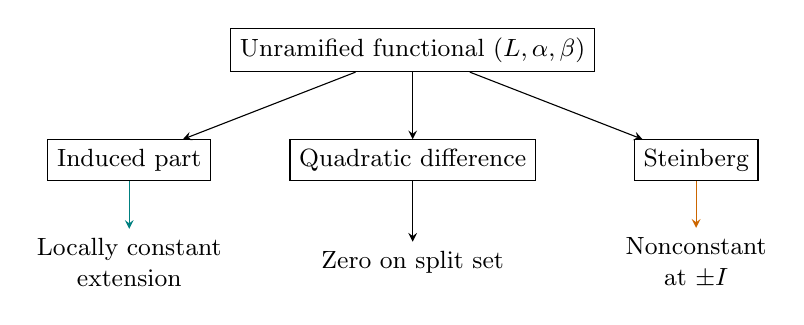
\begin{tikzpicture}[>=stealth,every node/.style={font=\small}]
\node[draw] (r) at (0,2.4) {Unramified functional $(L,\alpha,\beta)$};
\node[draw] (l) at (-3.6,1) {Induced part};
\node[draw] (d) at (0,1) {Quadratic difference};
\node[draw] (s) at (3.6,1) {Steinberg};
\foreach \v in {l,d,s}{\draw[->] (r)--(\v);}
\node[align=center] (lc) at (-3.6,-.3) {Locally constant\\extension};
\node (dc) at (0,-.3) {Zero on split set};
\node[align=center] (sc) at (3.6,-.3) {Nonconstant\\at $\pm I$};
\draw[->,teal] (l)--(lc);\draw[->] (d)--(dc);\draw[->,orange!80!black] (s)--(sc);
\end{tikzpicture}
\end{center}

\subsection{Character measures and higher spectral derivatives}
The original question about integrating characters is resolved for fixed finite Bernstein support by Theorem~\ref{thm:finite-block-admissibility}, rather than by assuming a uniform admissibility subgroup for an arbitrary family. A finite complex Borel measure on a compact tempered spectral subset of a block defines a functional by integration: for fixed $f$ the trace is bounded and Borel on the circle and at its finite exceptional points, by its polynomial coordinate and constituent values. Thus the integral exists. Finite support in the set of blocks makes the preceding theorem applicable. In the smooth block model the functional is continuous by the uniform norm estimate on the continuous coordinate and the ordinary finite-dimensional norms. This includes measures charging individual exceptional points, regardless of their Plancherel measure.

More generally, a distribution on the inducing unitary circle defines a spectral functional by pairing with the smooth total trace. It has finite distributional order on that compact circle. Theorem~\ref{thm:duality-moments} bounds its moments polynomially, and Theorem~\ref{thm:local-interpolation} supplies its local density. As an example take the $k$th angular derivative at $\theta_0$ of the total induced character. The unramified normalized split formula for $v(t)=m$ is
\[
2m^k\cos(m\theta_0+k\pi/2)
\]
for $k>0$, and $2\cos(m\theta_0)$ for $k=0$. For $k>0$ it vanishes on the regular split unit set. Such higher-order examples do not require a measure interpretation.

\subsection{Finite type and quasi-finite type}
The original notes express spectral distributions as derivatives of continuous functions on parameter tori. This can be retained in a precise Fourier form. For a bilateral sequence $m_n$ with polynomial bound of degree $N$, choose an integer $k>N+2$. After removing the constant mode, divide the Fourier coefficients of the distribution by $(in)^k$ for $n\ne0$. The resulting sequence is absolutely summable and hence defines a continuous periodic function. Its $k$th distributional derivative, plus the removed constant mode, is the original distribution (with Fourier sign conventions fixed consistently). The same argument applies to Weyl-invariant data by symmetrizing the derivative representation, or by choosing even $k$. The exceptional coordinates are separate scalars, not densities with respect to Plancherel measure.

We distinguish finite spectral type (finitely many nonzero blocks, each with polynomial moment growth), uniform quasi-finite spectral type (possibly infinitely many blocks but a common polynomial exponent, allowing block-dependent constants), and componentwise finite spectral order (each block has some polynomial exponent). These are refinements of the terminology of the original notes. The definition using derivatives of continuous functions also requires retaining the constant mode, and a uniform derivative order is equivalent to a uniform polynomial growth bound up to a fixed increase in the exponent.

\begin{center}
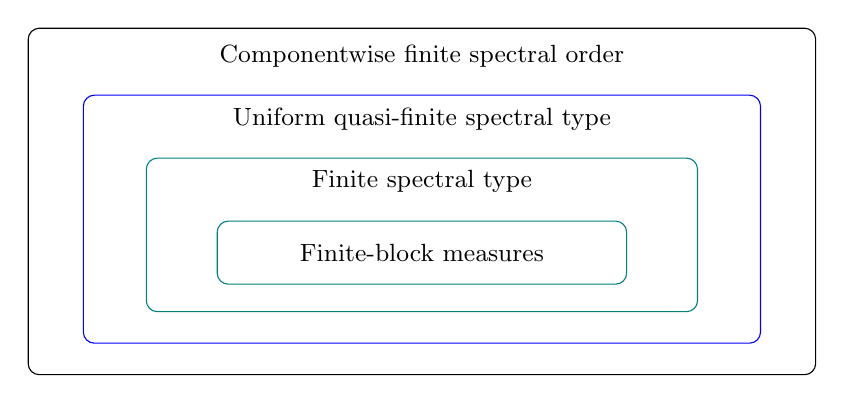
\begin{tikzpicture}[every node/.style={font=\small}]
\draw[rounded corners] (-5,-2.2) rectangle (5,2.2);
\node at (0,1.85) {Componentwise finite spectral order};
\draw[blue,rounded corners] (-4.3,-1.8) rectangle (4.3,1.35);
\node at (0,1.05) {Uniform quasi-finite spectral type};
\draw[teal,rounded corners] (-3.5,-1.4) rectangle (3.5,.55);
\node at (0,.25) {Finite spectral type};
\draw[teal,rounded corners] (-2.6,-1.05) rectangle (2.6,-.25);
\node at (0,-.65) {Finite-block measures};
\end{tikzpicture}
\end{center}
All three inclusions are strict at the spectral level. A derivative of a delta distribution on the circle need not be a finite measure, since its moments can be unbounded. Nonzero bounded sequences in infinitely many blocks give uniform quasi-finite but not finite type. Finally enumerate distinct generic ramified blocks by $\mathfrak s_j$, and take bilateral moments $m_{\mathfrak s_j,n}=n^{2j}$, $j\ge1$. Each block has finite order, but there is no uniform exponent. The interpretation of the last example as a group-side tempered distribution uses the global direct-sum topology and trace identification in Section~\ref{sec:tempered-duality}. The Plancherel measure need not be used as a reference measure for spectral distributions; multiplication or division by its density at singular points must be justified separately.

\subsection{Temperedness is not admissibility}
The point mass $\delta_I(f)=f(I)$ is invariant and continuous for the Schwartz topology: point evaluation is bounded by the defining seminorm on each fixed-level stage. It is not locally representable. Indeed, for a descending sequence of compact open neighborhoods $K_m$ of $I$, a locally integrable representative would satisfy $\int_{K_m}F(g)\,dg\to0$ by dominated convergence, while $\delta_I(\mathbf1_{K_m})=1$. Harish-Chandra regularity therefore rules out admissibility. By Plancherel inversion (with compatible Haar and Plancherel measures), it has the spectral expression
\[
\delta_I(f)=\int_{\widehat G_{\rm temp}}\Theta_\pi(f)\,d\mu_{\rm Pl}(\pi).
\]
The integral is the Plancherel trace formula, not a finite measure on the whole dual. Thus order zero on individual blocks does not guarantee local admissibility globally.

Conversely the trivial character is admissible but not tempered. The unramified polynomial moments of this character are $q^n+q^{-n}$ for $n\ge1$, with an independent coefficient $-1$ on the Steinberg trace. This violates the polynomial moment bound. This conclusion also follows directly from the ordinary non-temperedness of the trivial representation and the Schwartz trace theory.

\subsection{Central finiteness, block support and counterexamples}
Use the full Bernstein center, the product of the coordinate algebras of the components, acting on the algebraic trace space and its dual. Center-finite means that the orbit span of a functional under this center is finite-dimensional. The central block idempotents project a functional to its individual block components. Nonzero projections onto distinct blocks are linearly independent, so center-finiteness implies finite Bernstein support. By Theorem~\ref{thm:finite-block-admissibility}, it implies admissibility under the classical inputs of that theorem.

The converse fails. In the unramified block take
\[
L(Q)=\frac1{2\pi}\int_0^{2\pi}Q(2\cos\theta)\,d\theta,\qquad \alpha=\beta=0.
\]
This functional is a measure, is tempered in the smooth spectral model and is admissible by the finite-block theorem. If a nonzero polynomial $p$ annihilated $L$, taking $Q$ to have the conjugate coefficients of $p$ would give $\int |p(2\cos\theta)|^2\,d\theta=0$, a contradiction. Hence it is not center-finite. Center-finiteness does not imply temperedness either, as the trivial character illustrates.

\begin{center}
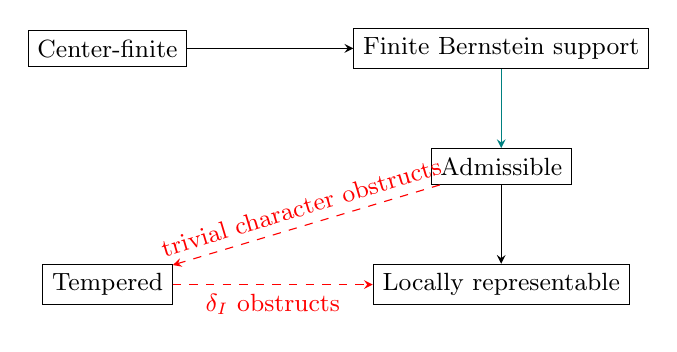
\begin{tikzpicture}[>=stealth,every node/.style={font=\small}]
\node[draw] (c) at (-3,2) {Center-finite};
\node[draw] (f) at (2,2) {Finite Bernstein support};
\node[draw] (a) at (2,.5) {Admissible};
\node[draw] (r) at (2,-1) {Locally representable};
\node[draw] (t) at (-3,-1) {Tempered};
\draw[->] (c)--(f);\draw[->,teal] (f)--(a);\draw[->] (a)--(r);
\draw[dashed,red,->] (t)--node[below] {$\delta_I$ obstructs}(r);
\draw[dashed,red,->] (a)--node[above,sloped] {trivial character obstructs}(t);
\end{tikzpicture}
\end{center}
Solid arrows denote implications using the indicated classical inputs; dashed red arrows denote false implications. Hecke-finiteness must be specified separately (for example by the precise fixed-level annihilation condition in a cited theorem). It is not a synonym for finite support or the proposed uniform quasi-finite spectral order. Its relation to center-finiteness in each block is discussed in Proposition~\ref{prop:hecke}.

\subsection{The original $\mathrm{GL}_2$ question}
The noncompact center in $\mathrm{GL}_2(F)$ motivates Fourier decomposition by central characters. For a test function $f$ and unitary central character $\omega$, the normalized central Fourier integral, when defined, is
\[
f_\omega(x)=\int_Z f(xz)\omega(z)^{-1}\,dz,\qquad
f_\omega(xz)=\omega(z)f_\omega(x).
\]
One cannot conclude that every distribution is an ordinary integral of pointwise distributions $D_\omega$; dependence on the central parameter may itself be distributional. Nor is a single global compact-open level automatic. A rank-two torus block suggests a corrected spectral model of smooth functions on $(S^1)^2$ with Weyl symmetry and the appropriate additional parameter spaces. Integration by parts and Fourier series give the elementary dual criterion
\[
|m_{j,k}|\le C(1+|j|+|k|)^N
\quad (j,k\in\mathbb Z).
\]
This is a torus calculation, not a proof of the full $\mathrm{GL}_2$ trace theorem. The original claim about quasi-finite representations of distributions is therefore retained as a research problem with invariant distributions and the actual topological trace space as necessary hypotheses.

\subsection{Remaining problems and literature}
The local interpolation theorem isolates the main rank-one input. Further work should check the exact Harish-Chandra admissibility definition and the classical character and restriction references, identify the full Schwartz topology, and investigate necessary conditions for admissibility of infinite-block distributions. In particular local finiteness of the character sums on open sets, not merely on individual test functions, is a useful candidate sufficient condition. Compare the normalized split restriction with normalized constant terms and Jacquet modules rather than identifying them at singular elements.

For broader context see Harish-Chandra \cite{HC99}, DeBacker's homogeneity results \cite{De02}, and the work on $\mathfrak z$-finite distributions by Aizenbud, Gourevitch and Sayag \cite{AGS15}. The recent preprint of Chen and Tsai \cite{CT26} on admissibility of Bernstein centers is particularly relevant to bounded spectral support. Its full text was not available for verification in the preceding literature pass; no theorem from it is used here. The relation between its center-valued distributions and the arbitrary scalar spectral functionals considered here must be checked. The group-side analytic growth question, the precise Hecke-finite formulation and the full $\mathrm{GL}_2$ extension remain open research directions rather than assertions of this paper.


% Section 9 of sl2-invariant-distributions-2026.tex.
% Developed by Claude (Fable, Anthropic), November 24, 2026. See revision_log.md.
\section{Supertempered distributions}\label{sec:supertemp}
The words \emph{tempered}, \emph{square-integrable}, \emph{elliptic}, \emph{cuspidal} and \emph{supertempered} denote distinct concepts. This section makes each of them explicit for $G=\mathrm{SL}_2(F)$ and determines how they are related. It uses the exceptional coordinates of Sections \ref{sec:spectral-geometry} and \ref{sec:pwcomparison}, the spectral duals of Sections \ref{sec:tempered-duality} and \ref{sec:admissible-duality}, and the descent theorems of Section \ref{sec:descent}.

Throughout this section $F$ is a finite extension of $\mathbb Q_p$ with $p$ odd. Characteristic zero is needed for the theorems of Herb and for the local character expansion. Write $A^0=a(\mathcal O^\times)$. Let $K_0=K=\mathrm{SL}_2(\mathcal O)$, let $K_1=gK_0g^{-1}$ with $g=\diag(\varpi,1)$ be the other maximal compact subgroup, and let $\mathcal I=K_0\cap K_1$ be the Iwahori subgroup. The Haar measure on $G$ gives $K_0$ volume one. As before $c=q+q^{-1}$ and $u=z+z^{-1}$.

Most of the structure below is the rank-one case of theorems of Harish-Chandra, Casselman, Kazhdan, Bernstein--Deligne--Kazhdan, Arthur, Herb and Schneider--Stuhler. The proofs given here are direct. Each depends on classical inputs, which are named where they are used. Subsection \ref{sub:st-status} lists the inputs whose exact statements still have to be checked against the sources. No claim of novelty is made.

\subsection{Six notions}\label{sub:six}
The words below are often used as if they were synonyms. In rank one each can be made completely explicit.

\begin{definition}\label{def:six}
Let $R(G)$ be the complexified Grothendieck group, $R_{\rm temp}(G)$ the span of the irreducible tempered classes, and $R_{\rm ind}(G)$ the span of the classes $[I(\chi)]$ for all quasicharacters $\chi$.
\begin{enumerate}[label=(\alph*),leftmargin=*]
\item A \emph{tempered invariant distribution} is a conjugation-invariant continuous functional on $\mathcal C(G)$. A \emph{tempered virtual character} is an element of $R_{\rm temp}(G)$, viewed as a distribution.
\item A tempered virtual character $\Theta$ is \emph{supertempered} if for every $r>0$ the function\[|\Delta_G(\gamma)|^{1/2}\,|\Theta(\gamma)|\,(1+\sigma(\gamma))^r\]is bounded on the regular set of every Cartan subgroup \cite{He94}. In $G$ only the split torus is noncompact, so the condition is that $h_\Theta(a(t))(1+|v(t)|)^r$ is bounded, where $h_\Theta(a)=|\Delta_G(a)|^{1/2}\Theta(a)$.
\item An irreducible tempered representation is \emph{elliptic} if its character is not identically zero on the regular elliptic set \cite{Ar93}.
\item The \emph{elliptic virtual characters} of Arthur are the $\Theta(M,\sigma,r)=\tr\bigl(R(r,\sigma)I_P(\sigma)\bigr)$ with $\sigma$ in the discrete series of $M$ and $r$ a regular element of the $R$-group. For $G$ they are the discrete series characters ($M=G$) and the three differences
\begin{equation}\label{eq:alt}
D_\eta=\Theta_{\pi_\eta^+}-\Theta_{\pi_\eta^-}
\end{equation}
attached to the nontrivial quadratic characters $\eta$ ($M=A$, $\sigma=\eta$, $r=w$).
\item A virtual character is \emph{cuspidal} if its normalized Jacquet module vanishes in $R(A)$, that is $r_B\Theta=0$. A \emph{supercuspidal character} is the character of an irreducible supercuspidal representation.
\item A distribution has \emph{elliptic support} if it is represented by a locally integrable function that vanishes on the regular split set. The \emph{elliptic class} of $\Theta\in R(G)$ is its image in $\overline R(G)=R(G)/R_{\rm ind}(G)$.
\end{enumerate}
\end{definition}
\begin{example}[Elliptic representations and elliptic virtual characters]\label{ex:supertemp}
Both $\pi_\eta^+$ and $\pi_\eta^-$ are elliptic tempered representations in the sense of (c), by Theorem \ref{thm:tree} below. Neither character is supertempered, since each has weak constant term $\eta$. Only their difference is. So ``elliptic representation'' and ``elliptic virtual character'' must not be merged. The Steinberg character is supertempered and is not cuspidal. The trivial character is not tempered, yet $\Theta_{\St}-\Theta_{\triv}$ is twice the natural algebraic representative of the elliptic class of $\St$ (Theorem \ref{thm:twosplit}).
\end{example}

\subsection{Constant terms: four functions on the torus}\label{sub:four}
Section \ref{sec:descent} separates the ordinary restriction, the normalized split restriction and the Jacquet-module constructions, and leaves their comparison open. In rank one the comparison is a table.

For a finite-length representation $\pi$ let $r_B(\pi)=\pi_N\otimes\delta_B^{-1/2}$ be the normalized Jacquet module, a finite-dimensional representation of $A\simeq F^\times$. Its \emph{exponents} are the characters that occur. For tempered $\pi$ let $r_B^w(\pi)$ be the sum of the generalized eigenspaces with unitary exponents. Herb's weak constant term is the character of the maximal tempered quotient of the normalized Jacquet module \cite[Section 2]{He94}, which has the same character. Put
\[
J_\pi=\tr r_B(\pi),\qquad \Theta_\pi^w=\tr r_B^w(\pi),\qquad h_\pi(a)=|\Delta_G(a)|^{1/2}\Theta_\pi(a)\quad(a\in A_{\rm reg}),
\]
and extend by linearity. The test-function side is Harish-Chandra's map $f\mapsto f^{(B)}$, with $f^{(B)}(a)=\delta_B(a)^{1/2}\int_N\int_K f(kank^{-1})\,dk\,dn$. It equals $F_f^A$ on $A_{\rm reg}$, lies in $C_c^\infty(A)$, and satisfies
\begin{equation}\label{eq:adj}
\Theta_{I(\chi)}(f)=\int_A\chi(a)f^{(B)}(a)\,da=\tfrac12\int_A(\chi+\chi^{-1})(a)\,f^{(B)}(a)\,da .
\end{equation}

\begin{proposition}[Casselman's theorem in rank one]\label{prop:cass}
Let $\Theta\in R(G)$. Then\[h_\Theta(a(t))=J_\Theta(a(t))\ \text{ for }|t|<1,\qquad h_\Theta(a(t))=J_\Theta(a(t^{-1}))\ \text{ for }|t|>1 .\]
\end{proposition}
This is \cite{Ca77}. Every regular $a(t)$ with $|t|\ne1$ is strictly contracting for $B$ or for the opposite Borel subgroup, so the theorem covers all of $A$ outside $A^0$. The statement agrees with the explicit characters of $I(\chi)$, $\St$, $\triv$ and $\pi_\eta^\pm$. On $A^0$ the two functions can differ. Call $E_\Theta=h_\Theta-J_\Theta$ on $A^0_{\rm reg}$ the \emph{compact defect}. It is well defined because $J_\Theta|_{A^0}$ is Weyl-invariant in every case below.

\begin{table}[htbp]\centering\small
\caption{The four functions on $A$. Here $|t|<1$ in the third column and $|t|=1$ in the last two. The supercuspidal row is for $\pi=\operatorname{c-Ind}_{K_0}^G\sigma$ with $\sigma$ cuspidal of dimension $q-1$ (Proposition \ref{prop:sc}).}\label{tab:four}
\begin{tabular}{@{}lllll@{}}\toprule
$\Theta$ & $J_\Theta$ & $h_\Theta$, $|t|<1$ & weak constant term & $E_\Theta$ on $A^0_{\rm reg}$\\\midrule
$I(\chi)$, $\chi$ unitary & $\chi+\chi^{-1}$ & $\chi+\chi^{-1}$ & $\chi+\chi^{-1}$ & $0$\\
$\pi_\eta^\pm$ & $\eta$ & $\eta$ & $\eta$ & $0$\\
$D_\eta$ & $0$ & $0$ & $0$ & $0$\\
$\St$ & $|t|$ & $|t|$ & $0$ & $1-|t-t^{-1}|$\\
$\triv$ & $|t|^{-1}$ & $|t|^{-1}$ & not defined & $|t-t^{-1}|-1$\\
supercuspidal $\pi$ & $0$ & $0$ & $0$ & $\omega_\pi(\pm1)(1-|t-t^{-1}|)$ on $\pm(1+\mathfrak p)$\\\bottomrule
\end{tabular}
\end{table}
The Jacquet characters come from the geometric lemma $r_B\,i_B\chi=\chi+\chi^{-1}$ in $R(A)$. At a quadratic point each constituent embeds in $I(\eta)$, so by Frobenius reciprocity each has a nonzero Jacquet module, and each gets one copy of $\eta$. At $|\cdot|^{\pm1}$ the trivial representation has $r_B(\triv)=\delta_B^{-1/2}=|\cdot|^{-1}$, which leaves $|\cdot|$ for Steinberg. The Steinberg row is the reason for the word ``weak'': its ordinary constant term is $|t|\neq0$ and its weak constant term is zero.

\begin{proposition}[Bohr-mean formula]\label{prop:bohr}Let $\Theta$ be a tempered virtual character. Then $h_\Theta(a(t))-\Theta^w(a(t))=\beta\,q^{-|v(t)|}$ for $v(t)\ne0$, where $\beta$ is the coefficient of $\Theta_{\St}$ in $\Theta$. Consequently, for every unitary character $\chi$ of $F^\times$, the coefficient of $\chi$ in $\Theta^w$ is
\[
\lim_{N\to\infty}\frac1N\sum_{m=1}^N\int_{\mathcal O^\times}h_\Theta\bigl(a(\varpi^mx)\bigr)\,\overline{\chi(\varpi^mx)}\,dx .
\]
\end{proposition}
\begin{proof}
By Proposition \ref{prop:cass}, $h_\Theta=J_\Theta$ for $|t|<1$. By Table \ref{tab:four} the only non-unitary exponent of a tempered irreducible representation is the exponent $|\cdot|$ of Steinberg. The Weyl symmetry of $h_\Theta$ gives $|t|>1$. The limit formula is orthogonality of characters on $\mathcal O^\times$ followed by a Ces\`aro mean in $m$, and the term $\beta q^{-m}$ has mean zero.
\end{proof}
So the weak constant term is the almost periodic part at infinity of the normalized split restriction. It is not the restriction itself, and it says nothing about $A^0$.

\subsection{Herb's theorem in rank one}\label{sub:herb}
\begin{theorem}[Herb \cite{He94}]\label{thm:herb}
Let $\mathbf G$ be a connected reductive group over a $p$-adic field of characteristic zero, and let $\Theta$ be a tempered virtual character of $\mathbf G(F)$.
\begin{enumerate}[label=(\alph*),leftmargin=*]
\item $\Theta$ is supertempered if and only if its weak constant terms along all proper parabolic subgroups vanish \cite[Theorem 2.5]{He94}.
\item The supertempered virtual characters are the finite linear combinations of Arthur's elliptic virtual characters $\Theta(M,\sigma,r)$ with $r$ regular \cite[Theorem 3.1]{He94}.
\item If $\Theta$ is supertempered and vanishes on the elliptic set, then $\Theta=0$ \cite[Theorem 3.2]{He94}.
\end{enumerate}
\end{theorem}
For $G=\mathrm{SL}_2(F)$ all three statements can be proved directly.

\begin{theorem}[Rank-one Herb theorem]\label{thm:herb-rank-one}For a tempered virtual character $\Theta=\sum_\pi a_\pi\Theta_\pi$ of $G$ the following are equivalent.
\begin{enumerate}[label=(\roman*),leftmargin=*]
\item $\Theta^w=0$.
\item $\Theta$ lies in $\ST(G)=\operatorname{span}\{\Theta_\pi:\pi\text{ discrete series}\}\oplus\bigoplus_{\eta}\mathbb C\,D_\eta$.
\item $\Theta$ is supertempered: $h_\Theta(a(t))(1+|v(t)|)^r$ is bounded for every $r$.
\item $|h_\Theta(a(t))|\le C\,q^{-|v(t)|}$ on $A_{\rm reg}$.
\end{enumerate}
\end{theorem}
\begin{proof}
The irreducible tempered representations are the irreducible unitary principal series $I(\chi)\simeq I(\chi^{-1})$, the six $\pi_\eta^\pm$, Steinberg and the supercuspidals. By Table \ref{tab:four},
\[
\Theta^w=\sum_{\{\chi,\chi^{-1}\},\,\chi^2\ne1}a_{I(\chi)}(\chi+\chi^{-1})+2a_{I(1)}\cdot1+\sum_\eta(a_{\pi_\eta^+}+a_{\pi_\eta^-})\,\eta .
\]
Distinct characters of $F^\times$ are linearly independent. So $\Theta^w=0$ if and only if every $a_{I(\chi)}$ vanishes and $a_{\pi_\eta^-}=-a_{\pi_\eta^+}$. This is (i)$\Leftrightarrow$(ii).

Assume (ii). By Proposition \ref{prop:bohr}, $h_\Theta(a(t))=\beta q^{-|v(t)|}$ for $v(t)\ne0$. On the compact set $A^0$ the function $h_\Theta$ is bounded, by Harish-Chandra's local boundedness of $|\Delta_G|^{1/2}\Theta_\pi$ \cite{HC99}. This gives (iv), and (iv) implies (iii).

Assume (iii). By Proposition \ref{prop:bohr}, $\Theta^w(a(t))\to0$ as $v(t)\to\infty$. Write $\Theta^w(a(\varpi^mx))=\sum_kC_k(x)z_k^m$ with distinct $z_k$ on the unit circle and $C_k$ finite combinations of characters of $\mathcal O^\times$. The Ces\`aro mean of $z_j^{-m}\sum_kC_k(x)z_k^m$ is $C_j(x)$ and is also zero. So every $C_j$ vanishes and $\Theta^w=0$.
\end{proof}

\begin{corollary}\label{cor:irr}An irreducible tempered character is supertempered if and only if the representation is in the discrete series. The supertempered virtual characters with support in the principal series blocks form a space of dimension four, with basis $\Theta_{\St},D_{\eta_\varepsilon},D_{\eta_\varpi},D_{\eta_{\varepsilon\varpi}}$.
\end{corollary}

Three natural questions arise. Does a supertempered virtual character that vanishes on the elliptic set vanish? Is a virtual character with vanishing constant term tempered? Is a virtual character with elliptic support supertempered?

\begin{corollary}[Answers to the three questions]\label{cor:three-questions}\begin{enumerate}[label=(\alph*),leftmargin=*]
\item If $\Theta$ is supertempered and vanishes on the regular elliptic set, then $\Theta=0$.
\item The kernel of $r_B$ on $R(G)$ is $\operatorname{span}\{\text{supercuspidal characters}\}\oplus\bigoplus_\eta\mathbb CD_\eta$. So a virtual character whose \emph{ordinary} constant term vanishes is automatically tempered and supertempered, and Steinberg is not of this kind.
\item A virtual character with elliptic support is cuspidal, hence tempered and supertempered.
\end{enumerate}
\end{corollary}
\begin{proof}
(a) If $\Theta$ vanishes on the elliptic set, the Weyl integration formula gives $\Theta(f)=\tfrac12\int_Ah_\Theta F_f^A$, which is zero for every $f$ with $f^{(B)}=0$. By the block descriptions of Subsection \ref{sec:pwcomparison} such $f$ realize arbitrary values of the coordinates $(0,d,b)$ and of finitely many supercuspidal traces. These are exactly the coefficients of an element of $\ST(G)$.

(b) Read off the coefficient of each character of $F^\times$ in $\sum a_\pi r_B(\pi)$, using $r_B(I(\chi))=\chi+\chi^{-1}$ for every irreducible $I(\chi)$, unitary or not, and Table \ref{tab:four}. The coefficients of $|\cdot|$ and $|\cdot|^{-1}$ are $a_{\St}$ and $a_{\triv}$.

(c) If $h_\Theta=0$ on $A_{\rm reg}$, then $J_\Theta$ vanishes for $|t|<1$ by Proposition \ref{prop:cass}. A finite combination of quasicharacters that vanishes on $\{|t|<1\}$ is zero. Now apply (b).
\end{proof}
Part (a) is \cite[Theorem 3.2]{He94} in rank one. Part (b) shows that the answer to the second question depends on the constant term used. With the ordinary constant term the answer is yes, and the resulting class excludes Steinberg. With the weak constant term temperedness is part of the definition. The converse of part (c) fails (Subsection \ref{sub:counter}).

\begin{figure}[htbp]\centering
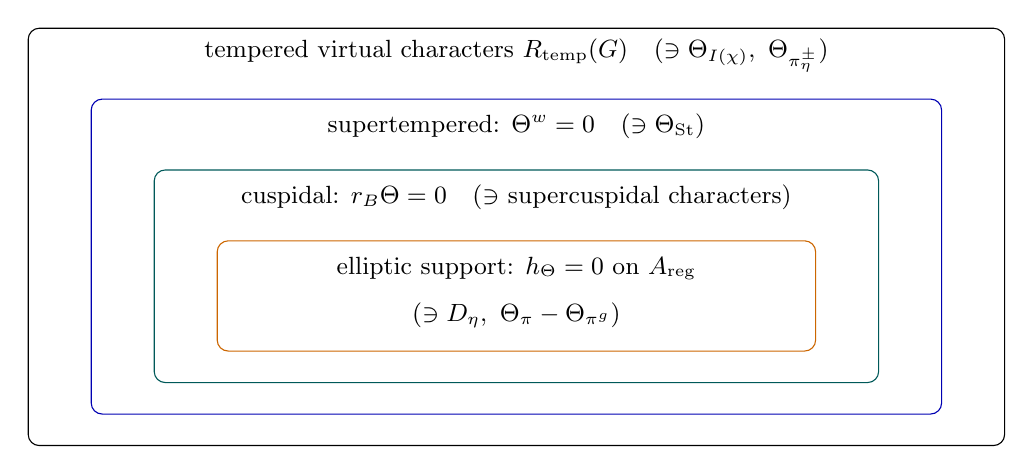
\begin{tikzpicture}[every node/.style={font=\small}]
\draw[rounded corners] (-6.2,-2.6) rectangle (6.2,2.7);
\node at (0,2.35) {tempered virtual characters $R_{\rm temp}(G)$\quad ($\ni\Theta_{I(\chi)},\ \Theta_{\pi_\eta^\pm}$)};
\draw[rounded corners,blue!70!black] (-5.4,-2.2) rectangle (5.4,1.8);
\node at (0,1.45) {supertempered: $\Theta^w=0$\quad ($\ni\Theta_{\St}$)};
\draw[rounded corners,teal!70!black] (-4.6,-1.8) rectangle (4.6,0.9);
\node at (0,.55) {cuspidal: $r_B\Theta=0$\quad ($\ni$ supercuspidal characters)};
\draw[rounded corners,orange!80!black] (-3.8,-1.4) rectangle (3.8,0);
\node at (0,-.35) {elliptic support: $h_\Theta=0$ on $A_{\rm reg}$};
\node at (0,-.95) {($\ni D_\eta,\ \Theta_{\pi}-\Theta_{\pi^g}$)};
\end{tikzpicture}
\caption{Four nested classes of tempered virtual characters. All inclusions are strict. Here $\pi^g$ is the conjugate of a depth-zero supercuspidal $\pi$ by $g=\diag(\varpi,1)$.}\label{fig:nested}
\end{figure}

\begin{remark}[Supertempered does not imply elliptic support]\label{rem:support}
The Steinberg character is supertempered and does not vanish on the regular split set. A supercuspidal character has vanishing Jacquet module and still does not vanish on the regular split set near $\pm I$ (Proposition \ref{prop:sc}). The weak-constant-term criterion is a condition at infinity on the split torus. It is not an elliptic-support criterion.
\end{remark}

\subsection{The quadratic constituents}\label{sub:quad}
The supertemperedness of $D_\eta$ has several proofs. Each shows something different, and all of them are given.

\begin{theorem}\label{thm:Deta}Let $\eta$ be a nontrivial quadratic character and $E_\eta=F(\sqrt\tau)$ the corresponding quadratic extension.
\begin{enumerate}[label=(\alph*),leftmargin=*]
\item $D_\eta^w=0$ and $r_B(D_\eta)=0$.
\item $D_\eta=\tr\bigl(R(w,\eta)I(\eta)(\cdot)\bigr)$, where $R(w,\eta)$ is the normalized self-intertwining operator with $R(w,\eta)^2=1$.
\item $D_\eta\circ\operatorname{Ad}(x)=\eta(\det x)\,D_\eta$ for $x\in\mathrm{GL}_2(F)$.
\item $D_\eta(\gamma)=0$ for every regular semisimple $\gamma$ whose centralizer in $\mathrm{GL}_2(F)$ contains an element $x$ with $\eta(\det x)=-1$. This holds for all regular split $\gamma$ and for all regular elliptic $\gamma$ in tori that do not split over $E_\eta$.
\end{enumerate}
\end{theorem}
\begin{proof}
(a) is Table \ref{tab:four}. For (b), the commuting algebra of $I(\eta)$ has dimension two, by Frobenius reciprocity and $r_B\,I(\eta)=2\eta$, and it is spanned by $1$ and $R(w,\eta)$ \cite{Ke82}. The two constituents are the eigenspaces of $R(w,\eta)$ for $\pm1$. The operator acts on the two-dimensional Jacquet module with eigenvalues $+1$ and $-1$, so its trace there is zero. This is a second proof of (a).

(c) The argument before Theorem \ref{thm:unramified-descent} shows that $\mathrm{GL}_2(F)$ permutes $\{\pi_\eta^+,\pi_\eta^-\}$ transitively. The stabilizer of $\pi_\eta^+$ contains $\mathrm{SL}_2(F)$ and the center, and has index two. The irreducible principal series $I_{\mathrm{GL}_2}(\eta,1)$ is isomorphic to its twist by $\eta\circ\det$ and by no other nontrivial character of $F^\times/F^{\times2}$. By Clifford theory the stabilizer is the kernel of $\eta\circ\det$.

(d) Apply (c) with $x$ in the centralizer of $\gamma$. For split $\gamma=a(t)$ take $x=\diag(y,1)$ with $\eta(y)=-1$. For $\gamma$ in an elliptic torus attached to a quadratic extension $E'$, the centralizer is $E'^\times$ and $\det$ is the norm. If $E'\ne E_\eta$ then $\eta$ is nontrivial on the norms from $E'$.
\end{proof}
Part (d) is stronger than supertemperedness. It gives elliptic support, and it locates the support on the tori that split over $E_\eta$. This is the pattern of the Sally--Shalika formulas \cite{SS68} and of the endoscopic description of the packet $\{\pi_\eta^+,\pi_\eta^-\}$ \cite{LL79}.

For the unramified character $\eta_\varepsilon$ the values on the support can be computed by hand. Label the constituents so that $\pi_+$ has a $K_0$-fixed vector. Then $\pi_-$ has a $K_1$-fixed vector, by (c) with $x=\diag(\varpi,1)$. Let $X$ be the Bruhat--Tits tree. Its vertices have type $0$ or $1$ according to whether their stabilizer is conjugate in $G$ to $K_0$ or $K_1$. Adjacent vertices have different types. For a compact element $\gamma$ let $V_i(\gamma)$ be the number of fixed vertices of type $i$.

\begin{theorem}[Tree formula]\label{thm:tree}For every regular elliptic $\gamma$,
\[
\Theta_{\pi_\pm}(\gamma)=\pm\bigl(V_0(\gamma)-V_1(\gamma)\bigr),\qquad D_{\eta_\varepsilon}(\gamma)=2\bigl(V_0(\gamma)-V_1(\gamma)\bigr),\qquad \Theta_{\St}(\gamma)=-1 .
\]
If $\gamma$ lies in an unramified elliptic torus and its fixed set is the ball of radius $n$ around a vertex of type $i$, then $D_{\eta_\varepsilon}(\gamma)=2(-1)^i(-q)^n=2(-1)^{i+n}|\Delta_G(\gamma)|^{-1/2}$. If $\gamma$ lies in a ramified elliptic torus, then $D_{\eta_\varepsilon}(\gamma)=0$.
\end{theorem}
\begin{proof}
For a depth-zero representation $V$ and elliptic regular $\gamma$, Schneider and Stuhler prove
\[
\Theta_V(\gamma)=\sum_{x}\tr\bigl(\gamma\mid V^{K_x^+}\bigr)-\sum_{e}\tr\bigl(\gamma\mid V^{\mathcal I_e^+}\bigr),
\]
the sums running over the fixed vertices and fixed edges, with $K_x^+$ and $\mathcal I_e^+$ the pro-unipotent radicals \cite[Section III.4]{SS97}. The space $I(\eta_\varepsilon)^{K_0^+}$ is the representation of $\mathrm{SL}_2(\mathbb F_q)$ induced from the trivial character of the Borel subgroup, which is $\triv\oplus\St_q$. Each of $\pi_\pm$ has a one-dimensional space of $\mathcal I$-fixed vectors. So $\pi_+^{K_x^+}$ is $\triv$ at vertices of type $0$ and $\St_q$ at vertices of type $1$, and $\pi_-$ is the reverse. Edge spaces are one-dimensional with trivial action. The value of $\St_q$ at the reduction of $\gamma$ at $x$ is the number of fixed points on $\mathbb P^1(\mathbb F_q)$ minus one, which is $\deg(x)-1$ with $\deg$ the degree in the fixed tree. Let $E$ be the number of fixed edges. Each edge has one endpoint of each type, so $\sum_{\text{type }1}\deg(x)=E$. Hence
\[
\Theta_{\pi_+}(\gamma)=V_0+(E-V_1)-E=V_0-V_1 .
\]
The same computation gives $\Theta_{\St}(\gamma)=\sum_x(\deg(x)-1)-E=E-(V_0+V_1)=-1$, the Euler characteristic of a finite tree with the sign reversed.

In a ball of radius $n$ around a vertex of type $i$ the sphere of radius $j\ge1$ has $(q+1)q^{j-1}$ vertices of type $i+j$. The alternating sum $1-(q+1)+(q+1)q-\cdots$ up to radius $n$ is $(-q)^n$. For such $\gamma$ one has $|\Delta_G(\gamma)|^{1/2}=q^{-n}$. A ramified elliptic element fixes a ball centered at the midpoint of an edge. Reflection in the midpoint is a bijection of that ball that exchanges types, so $V_0=V_1$.
\end{proof}
The two $G$-conjugacy classes of unramified elliptic tori are distinguished by the type $i$ of the vertex they fix, and $D_{\eta_\varepsilon}$ has opposite signs on them. The same method on a ball-truncated apartment, justified by Korman's theorem for compact elements in rank one \cite{Ko04}, gives $\Theta_{\St}(a(t))=2q^n-1$ and $\Theta_{\pi_\pm}(a(t))=q^n$ for $t\in1+\mathfrak p^n$, $t\notin 1+\mathfrak p^{n+1}$. These agree with the classical formulas, which checks the normalization.

\begin{proposition}[Explicit pseudo-coefficients]\label{prop:pseudo}Let $e_J=\vol(J)^{-1}\mathbf 1_J$. The functions
\[
f_-=e_{K_0}-e_{K_1},\qquad f_{\St}=e_{\mathcal I}-e_{K_0}-e_{K_1}
\]
have $f^{(B)}=0$. In the unramified block coordinates $(Q,d,b)$ of Subsection \ref{sec:pwcomparison} they are $(0,2,0)$ and $(0,0,1)$, and their traces on all other blocks vanish. For elliptic regular $\gamma$ with $\vol(G_\gamma)=1$, $\mathcal O_\gamma(f_-)=V_0(\gamma)-V_1(\gamma)=\tfrac12D_{\eta_\varepsilon}(\gamma)$.
\end{proposition}
\begin{proof}
For unramified $\chi$, $\dim I(\chi)^{K_i}=1$ and $\dim I(\chi)^{\mathcal I}=2$. So both functions have trace zero on every $I(\chi)$, and by \eqref{eq:adj} and Mellin inversion $f^{(B)}=0$. Representations outside the unramified block have no $\mathcal I$-fixed vectors. The traces on $\pi_+,\pi_-,\St,\triv$ are $(1,-1,0,0)$ for $f_-$ and $(0,0,1,-1)$ for $f_{\St}$. The orbital integral of $e_{K_i}$ counts fixed vertices of type $i$.
\end{proof}
The function $-f_{\St}$ is Kottwitz's Euler--Poincar\'e function \cite{Ko88}. The formula for $\mathcal O_\gamma(f_-)$ is an instance of Kazhdan's orthogonality \cite{Ka86,SS97}, since $\|D_{\eta_\varepsilon}\|^2_{\rm ell}=4$ and $D_{\eta_\varepsilon}(f_-)=2$.

\subsection{The elliptic quotient and its two splittings}\label{sub:split}
This subsection answers the question raised at the end of Section \ref{sec:admissible-duality}: what do the exceptional coordinates characterize?

Define two operators, the first on $R(G)$ and the second on $R_{\rm temp}(G)$:
\[
\mathsf A=1-\tfrac12\,i_B\,r_B,\qquad \mathsf A^w=1-\tfrac12\,i_B\,r_B^w .
\]
The first is the rank-one case of the operator used by Bernstein, Deligne and Kazhdan to isolate the elliptic part \cite{BDK86,Da00}.

\begin{theorem}[Two complements of the induced part]\label{thm:twosplit}\begin{enumerate}[label=(\alph*),leftmargin=*]
\item $\mathsf A$ is idempotent with kernel $R_{\rm ind}(G)$. Its image $R_{\rm ell}(G)=\ker(i_Br_B)$ has basis the supercuspidal classes, the three $D_\eta$, and $\St-\triv$.
\item $\mathsf A^w$ is idempotent with kernel $R_{\rm ind}(G)\cap R_{\rm temp}(G)$ and image $\ST(G)$.
\item Both $R_{\rm ell}(G)$ and $\ST(G)$ map isomorphically onto the elliptic quotient $\overline R(G)$. The resulting isomorphism $\ST(G)\to R_{\rm ell}(G)$ is $\Theta\mapsto\mathsf A\Theta$. It is the identity on supercuspidal characters and on the $D_\eta$, and it sends $\St$ to $\tfrac12(\St-\triv)$.
\item For tempered $\Theta$ with Steinberg coefficient $\beta$, $\ \mathsf A^w\Theta-\mathsf A\Theta=\tfrac\beta2\,[I(|\cdot|)]$.
\end{enumerate}
\end{theorem}
\begin{proof}
In $R(A)$, $r_B\,i_B=1+w$, and $i_B\circ w=i_B$ in $R(G)$. So $\mathsf A\,i_B=i_B-\tfrac12(i_B+i_Bw)=0$ and $\mathsf A^2=\mathsf A-\tfrac12\mathsf A\,i_Br_B=\mathsf A$. The kernel is contained in the image of $i_B$ and contains it. The image is $\{x:i_Br_Bx=0\}$. Evaluating $\mathsf A$ on irreducibles gives $\mathsf A(\pi_\eta^\pm)=\pm\tfrac12D_\eta$, $\mathsf A(\St)=\tfrac12(\St-\triv)=-\mathsf A(\triv)$, $\mathsf A(\pi)=\pi$ for supercuspidal $\pi$, and $\mathsf A(I(\chi))=0$. This is (a). The same argument with $r_B^wi_B\chi=\chi+\chi^{-1}$ for unitary $\chi$ gives (b), and the image is $\ker r_B^w=\ST(G)$ by Theorem \ref{thm:herb-rank-one}. Part (c) follows because both are complements of the same kernel. Part (d) is $\tfrac12i_B(r_B-r_B^w)\Theta$ and Table \ref{tab:four}.
\end{proof}

In the language of the earlier sections, the coordinate $b=\tr\St$ is the functional $\Theta_{\St}\in\ST(G)$, and the coordinate $d_{\St}=\tr\St-\tr\triv$ of Subsection \ref{subsec:pw-coordinates} is the functional $2\mathsf A(\St)\in R_{\rm ell}(G)$. Both represent the same class modulo functionals of the induced trace $Q$, because $\Theta_{\triv}=\ev_c-\Theta_{\St}$. The phrase ``functionals with zero polynomial moments'' therefore depends on the coordinates chosen. With $(Q,d,b)$ it means $\ST$. With $(Q,d,d_{\St})$ it means $R_{\rm ell}$. With $(Q,d,t)$, $t=\tr\triv$, it would be the span of $D_\eta$ and the trivial character. Only the quotient is intrinsic. Temperedness selects $\ST$, and compatibility with Jacquet restriction selects $R_{\rm ell}$.

Now pass to functionals. For a Bernstein block $\mathfrak s$ let $\PW^{\mathfrak s}$ be the algebraic trace space of Subsection \ref{sec:pwcomparison}. Let $\PW^{\mathfrak s}_c$ be the subspace of trace forms vanishing on every $[I(\chi)]$, and $\PW^{\mathfrak s}_{\rm ind}=\PW^{\mathfrak s}/\PW^{\mathfrak s}_c$, the space of induced trace polynomials.

\begin{theorem}[Exact sequences and annihilators]\label{thm:exact}
Assume the algebraic block descriptions of Subsection \ref{sec:pwcomparison}.For every block $\mathfrak s$ there are exact sequences, dual to each other,
\[
0\to\PW_c^{\mathfrak s}\to\PW^{\mathfrak s}\to\PW^{\mathfrak s}_{\rm ind}\to0,\qquad
0\to(\PW^{\mathfrak s}_{\rm ind})'\to(\PW^{\mathfrak s})'\to(\PW^{\mathfrak s}_c)'\to0 .
\]
The space $\PW_c^{\mathfrak s}$ is finite-dimensional and $(\PW_c^{\mathfrak s})'\simeq\overline R(G)^{\mathfrak s}$. Moreover:
\begin{enumerate}[label=(\alph*),leftmargin=*]
\item $(\PW^{\mathfrak s}_{\rm ind})'=\Ann(\PW^{\mathfrak s}_c)$. These are the functionals $D_L$ of Theorem \ref{thm:local-interpolation}.
\item $(\PW^{\mathfrak s})'=(\PW^{\mathfrak s}_{\rm ind})'\oplus\ST^{\mathfrak s}$, and $\ST^{\mathfrak s}=\Ann(N^{\mathfrak s}_{\rm temp})$, where $N^{\mathfrak s}_{\rm temp}$ is the space of trace forms $\pi\mapsto\tfrac12\psi(r_B^w\pi)$ on tempered $\pi$, with $\psi$ a Weyl-invariant regular function on the twist torus. In the unramified block $N_{\rm temp}=\{(Q,0,0)\}$.
\item $(\PW^{\mathfrak s})'=(\PW^{\mathfrak s}_{\rm ind})'\oplus R^{\mathfrak s}_{\rm ell}$, and $R_{\rm ell}^{\mathfrak s}=\Ann(N^{\mathfrak s}_{\rm alg})$, where $N^{\mathfrak s}_{\rm alg}$ is the space of trace forms $\pi\mapsto\tfrac12\psi(r_B\pi)$. In the unramified block $N_{\rm alg}=\{(Q,0,\tfrac12Q(c))\}$.
\end{enumerate}
\begin{center}\small
\begin{tabular}{@{}lcccl@{}}\toprule
Block & $\PW_{\rm ind}^{\mathfrak s}$ & $\dim\PW_c^{\mathfrak s}$ & isolated points of $T_{\mathfrak s}/\!/W_{\mathfrak s}$ & basis of $\ST^{\mathfrak s}$\\\midrule
supercuspidal & $0$ & $1$ & $1$ & $\Theta_\pi$\\
I, $\xi^2\ne1$ & $\mathbb C[z,z^{-1}]$ & $0$ & $0$ & none\\
II, $\xi^2=1\ne\xi$ & $\mathbb C[u]$ & $2$ & $2$ & $D_\eta$ at $z=1$ and at $z=-1$\\
III, $\xi=1$ & $\mathbb C[u]$ & $2$ & $2$ & $D_{\eta_\varepsilon}$, $\Theta_{\St}$\\\bottomrule
\end{tabular}
\end{center}
\end{theorem}
\begin{proof}
Exactness is the definition. In coordinates, $\PW_c$ is $\{Q=0\}$, and $N_{\rm temp}$, $N_{\rm alg}$ are complements of it, as one sees by evaluating $\tfrac12\psi\circ r_B^w$ and $\tfrac12\psi\circ r_B$ on $\pi_\pm$, $\St$, $\triv$ with Table \ref{tab:four}. The annihilator of a complement of $\PW_c$ is a complement of $\Ann(\PW_c)$ that maps isomorphically to $(\PW_c)'$. The functionals $d$ and $b$ vanish on $N_{\rm temp}$, and $d$ and $2b-\ev_c$ vanish on $N_{\rm alg}$.
\end{proof}
So supertempered characters are annihilators of induced trace data, in a precise sense: they kill the trace forms that factor through the weak Jacquet functor. The extended quotient of Subsection \ref{subsec:extended-quotient} counts them. In Type II both isolated points carry a nontrivial $R$-group. In Type III the point $e_-$ carries $D_{\eta_\varepsilon}$, and the point $e_+$ at $z=1$, where the $R$-group is trivial, carries Steinberg after the correcting cocharacter moves its support to $c$. The count $4=1+3$ of Corollary \ref{cor:irr} is also the number of elliptic endoscopic data of $\mathrm{SL}_2$: the group itself and the three norm-one tori \cite{LL79}.

\begin{figure}[htbp]\centering
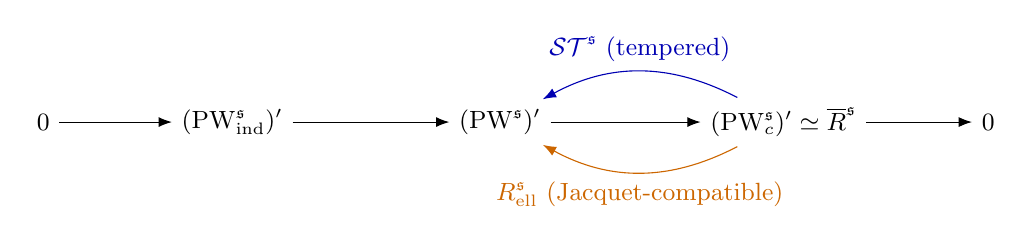
\begin{tikzpicture}[>=Latex,every node/.style={font=\small}]
\node (a) at (0,0) {$0$};
\node (b) at (2.4,0) {$(\PW_{\rm ind}^{\mathfrak s})'$};
\node (c) at (5.8,0) {$(\PW^{\mathfrak s})'$};
\node (d) at (9.4,0) {$(\PW_c^{\mathfrak s})'\simeq\overline R^{\mathfrak s}$};
\node (e) at (12,0) {$0$};
\draw[->] (a)--(b);\draw[->] (b)--(c);\draw[->] (c)--(d);\draw[->] (d)--(e);
\draw[->,blue!70!black,bend right=28] (d) to node[above] {$\ST^{\mathfrak s}$ (tempered)} (c);
\draw[->,orange!80!black,bend left=28] (d) to node[below] {$R^{\mathfrak s}_{\rm ell}$ (Jacquet-compatible)} (c);
\end{tikzpicture}
\caption{One quotient, two splittings. Their difference is $\beta\mapsto\frac\beta2\ev_c$ on the Steinberg line and zero elsewhere.}\label{fig:splittings}
\end{figure}

\subsection{The weak constant term of a distribution}\label{sub:wct}
Herb defines weak constant terms for virtual characters. Section \ref{sec:descent} treats arbitrary spectral functionals. The two meet as follows. Let $D$ be an invariant distribution supported in a principal series block with unit character $\xi$. By Theorem \ref{thm:exact}(b) write $D=D_L+\Theta^{\rm st}$ uniquely, with $L$ a functional on the induced trace polynomial and $\Theta^{\rm st}\in\ST^{\mathfrak s}$.

\begin{definition}\label{def:wct}
The \emph{weak constant term} of $D$ is the function on $A$
\[
D^w_B(a(t))=L\bigl(z\mapsto\chi_{\xi,z}(t)+\chi_{\xi,z}(t)^{-1}\bigr).
\]
In the unramified block, with $m_n=L(B_n)$, this is $m_{|v(t)|}$ for $v(t)\ne0$ and $2m_0$ on $A^0$.
\end{definition}

\begin{theorem}[Canonical decomposition]\label{thm:decomp}
Part (e) is conditional on the Schwartz trace identification of Section \ref{sec:tempered-duality}.
\begin{enumerate}[label=(\alph*),leftmargin=*]
\item $D^w_B$ is a Weyl-invariant locally constant function on all of $A$, including $\pm I$.
\item For every $f\in C_c^\infty(G)$, $\ D(f)=\tfrac12\int_AD^w_B(a)\,f^{(B)}(a)\,da+\Theta^{\rm st}(f)$.
\item If $D$ is a tempered virtual character, $D^w_B$ is Herb's weak constant term.
\item On $A_{\rm reg}$, $h_D=D^w_B+h_{\Theta^{\rm st}}$, and $h_{\Theta^{\rm st}}(a(t))=\beta q^{-|v(t)|}$ for $v(t)\ne0$.
\item In the smooth model of Section \ref{sec:tempered-duality}, $D$ is tempered if and only if $|D^w_B(a(t))|\le C(1+|v(t)|)^N$.
\item $D^w_B=0$ if and only if $D\in\ST^{\mathfrak s}$.
\end{enumerate}
\end{theorem}
\begin{proof}
(a) is Theorem \ref{thm:induced-descent}. For (b), $f^{(B)}$ is locally constant with compact support, so the integral in \eqref{eq:adj} is a finite sum of terms $\chi_{\xi,z}(a_j)c_j$, and $L$ may be applied term by term. For (c) take $L=\ev_{z_0}$ and use Table \ref{tab:four}, with $\pi_\eta^\pm=\tfrac12I(\eta)\pm\tfrac12D_\eta$. Part (d) is Theorem \ref{thm:local-interpolation} together with Proposition \ref{prop:bohr}. Part (e) is Theorem \ref{thm:duality-moments}. Part (f) holds because $L$ is determined by its moments.
\end{proof}
Thus the descent theorem of Section \ref{sec:descent} is a statement about weak constant terms: the weak constant term of a finite-block distribution is an admissible distribution on $A$, and the distribution is supertempered when it vanishes. For a non-tempered virtual character the same formula gives its induced part relative to the tempered splitting. For example $\Theta_{\triv}$ has $D^w_B=|t|+|t|^{-1}$ and $\Theta^{\rm st}=-\Theta_{\St}$.

\subsection{Singular behavior at $\pm I$}\label{sub:germ}
The weak constant term sees only infinity. Near $\pm I$ a different invariant governs, and it is not zero for supertempered characters.

\begin{theorem}[Split germ at the identity]\label{thm:germ}For every $\Theta\in R(G)$ there are constants $w(\Theta)$ and $c_0(\Theta)$ and a neighborhood of $1$ in $F^\times$ on which
\[
h_\Theta(a(t))=\tfrac12\,w(\Theta)+c_0(\Theta)\,|t-t^{-1}|\qquad(t\ne1).
\]
Here $c_0(\Theta)$ is the coefficient of the trivial nilpotent orbit in the Harish-Chandra--Howe expansion, and $w(\Theta)=\sum_{\mathcal O}c_{\mathcal O}(\Theta)$ is the sum over the four regular nilpotent orbits. For irreducible $\pi$, $h_\pi(-a(t))=\omega_\pi(-1)h_\pi(a(t))$ gives the expansion at $-I$.
\end{theorem}
\begin{proof}
Near the identity $\Theta(\exp X)=c_0+\sum_{\mathcal O}c_{\mathcal O}\widehat\mu_{\mathcal O}(X)$ \cite{HC99}. For a regular nilpotent orbit, $\widehat\mu_{\mathcal O}(sX)=|s|^{-1}\widehat\mu_{s\mathcal O}(X)$. Conjugation by $\diag(1,s)$ fixes the split element $X_x=\diag(x,-x)$, preserves the invariant form, and permutes the four regular orbits transitively. So the four functions $\widehat\mu_{\mathcal O}$ agree on the split Cartan subalgebra, and $\widehat\mu_{\mathcal O}(X_{sx})=|s|^{-1}\widehat\mu_{\mathcal O}(X_x)$ for all $s$. Hence $\widehat\mu_{\mathcal O}(X_x)=\kappa/|2x|$ with one constant $\kappa$. The case $\Theta=\Theta_{I(\chi)}$, where $h=\chi+\chi^{-1}\to2$ and all four coefficients are $1$, gives $\kappa=\tfrac12$.
\end{proof}

\begin{center}\small
\begin{tabular}{@{}lccl@{}}\toprule
$\pi$ & $w(\pi)$ & $c_0(\pi)$ & source of the values\\\midrule
$I(\chi)$ irreducible & $4$ & $0$ & character formula\\
$\pi_\eta^\pm$ & $2$ & $0$ & $h=\eta$\\
$\St$ & $4$ & $-1$ & $h=2-|t-t^{-1}|$\\
$\triv$ & $0$ & $1$ & $h=|t-t^{-1}|$\\
discrete series $\pi$ & $1$, $2$ or $4$ & $-d(\pi)/d(\St)$ & Harish-Chandra; Rodier\\\bottomrule
\end{tabular}
\end{center}
By Rodier's theorem $w(\pi)$ is the number of classes $a\in F^\times/F^{\times2}$ for which $\pi$ has a Whittaker model with respect to $\psi_a$ \cite{Ro75}. The formula $c_0(\pi)=-d(\pi)/d(\St)$ for the discrete series is Harish-Chandra's \cite{HC99}. With $\vol(K_0)=1$ the Euler--Poincar\'e measure gives $d(\St)=q-1$. Both are confirmed independently by the next proposition.

\begin{proposition}[A depth-zero supercuspidal character on the split torus]\label{prop:sc}Let $\sigma$ be a cuspidal representation of $\mathrm{SL}_2(\mathbb F_q)$ of dimension $q-1$, inflated to $K_0$, and $\pi=\operatorname{c-Ind}_{K_0}^G\sigma$. For $t\in\mathcal O^\times$, $t\ne\pm1$,
\[
\Theta_\pi(a(t))=\begin{cases}\omega_\pi(\pm1)\bigl(|t-t^{-1}|^{-1}-1\bigr),&t\in\pm(1+\mathfrak p),\\ 0,&t\not\equiv\pm1\bmod\mathfrak p,\end{cases}
\]
and $\Theta_\pi(a(t))=0$ for $|t|\ne1$. So $w(\pi)=2$ and $c_0(\pi)=-1=-d(\pi)/d(\St)$. The same formula holds for the sum of the two cuspidal representations of dimension $(q-1)/2$.
\end{proposition}
\begin{proof}
Only vertices of type $0$ contribute, with $\pi^{K_x^+}\simeq\sigma$, and edges contribute nothing because $\sigma$ has no vector fixed by the unipotent radical. Let $t\in1+\mathfrak p^n$, $t\notin1+\mathfrak p^{n+1}$. The fixed set of $a(t)$ is the set of vertices at distance at most $n$ from the standard apartment. At distance $j<n$ the element reduces to the identity, with trace $q-1$. At distance $n$ it reduces to a nontrivial unipotent, with trace $-1$. There are $(q-1)q^{j-1}$ vertices at distance $j\ge1$ over each apartment vertex, and the type is the parity of position plus distance. Truncate at the ball of radius $R$ around a vertex of the apartment. A pair of adjacent complete columns contributes zero. The incomplete columns at the two ends contribute a total that is independent of $R$, and the sum is $q^n-1$. For $t\not\equiv\pm1$ the fixed set is the apartment and the trace of $\sigma$ at a regular split element is zero. The case $|t|\ne1$ is Proposition \ref{prop:cass}.
\end{proof}
The sum $q^n-1$, and the corresponding values $2q^n-1$ for Steinberg and $1$ for the trivial representation, were checked by exact computation for $q\in\{3,5,7\}$, $n\le4$ and several $R$. A comparison with the tables of \cite{SS68,ADSS11} has not been made.

\begin{corollary}[Split descent criterion]\label{cor:descent}Let $\Theta=\sum a_\pi\Theta_\pi$ be a virtual character. Its normalized split restriction extends to a locally constant function on all of $A$ if and only if
\[
\sum_\pi a_\pi\,c_0(\pi)=0\quad\text{and}\quad\sum_\pi a_\pi\,\omega_\pi(-1)\,c_0(\pi)=0 .
\]
For supertempered $\Theta$ this reads $\sum a_\pi\,\omega_\pi(\pm1)\,d(\pi)=0$, the sums over the discrete series. For an invariant distribution with finite Bernstein support the criterion applies to its part $\Theta^{\rm st}$, because the induced part always descends (Theorem \ref{thm:decomp}(a)).
\end{corollary}
Within the unramified block the criterion is $\beta=0$, which is Theorem \ref{thm:unramified-descent}. Across blocks the Steinberg obstruction can cancel.
\begin{example}[Steinberg minus a supercuspidal]\label{ex:cancel}
Let $F=\mathbb Q_5$ and let $\theta$ be a character of order three of the group $\mu_6$ of norm-one elements of $\mathbb F_{25}$. Then $\theta(-1)=1$, the cuspidal representation $\sigma_\theta$ has dimension $4$, and $\pi=\operatorname{c-Ind}\sigma_\theta$ has $\omega_\pi(-1)=1$. By Table \ref{tab:four}, $\Theta_{\St}-\Theta_\pi$ has
\[
h(a(t))=5^{-|v(t)|}\quad\text{for all regular }t .
\]
It is locally constant across $\pm I$ although the Steinberg coefficient is $1$. Over $\mathbb Q_3$ the only cuspidal representation of dimension $q-1=2$ has $\omega(-1)=-1$. There one uses $\Theta_{\St}-\Theta_{\pi_0^+}-\Theta_{\pi_0^-}$, with $\pi_0^\pm$ induced from the two nontrivial one-dimensional characters of $\mathrm{SL}_2(\mathbb F_3)$, and obtains $h(a(t))=3^{-|v(t)|}$.
\end{example}
\begin{figure}[htbp]\centering
\begin{tikzpicture}[x=1.3cm,y=1.6cm,>=Latex,every node/.style={font=\small}]
\draw[->] (0.5,0)--(6.8,0) node[right]{$n$};
\draw[->] (0.5,0)--(0.5,2.35) node[above]{$h(a(1+5^n))$};
\foreach \y in {1,2}{\draw (0.42,\y)--(0.58,\y) node[left,xshift=-4pt]{\y};}
\foreach \n/\s in {1/0.2,2/0.04,3/0.008,4/0.0016,5/0.0003,6/0.0001}{
\fill[blue!70!black] (\n,{2-\s}) circle (1.6pt);
\fill[teal!70!black] (\n,{1-\s}) circle (1.6pt);
\draw[orange!80!black,thick] (\n-0.08,1.03)--(\n+0.08,1.03);
\node[below] at (\n,0) {\n};}
\node[blue!70!black,anchor=west] at (2.3,2.17) {$\St$: $2-5^{-n}$};
\node[teal!70!black,anchor=west] at (2.3,0.72) {$\pi$: $1-5^{-n}$};
\node[orange!80!black,anchor=west] at (2.3,1.25) {$\St-\pi$: constant $1$};
\end{tikzpicture}
\caption{Normalized split restrictions along $t=1+5^n$ in $\mathbb Q_5$. Each discrete series character fails to be locally constant at $I$. The difference is constant.}\label{fig:cancel}
\end{figure}

\subsection{The Bernstein center and Hecke-finiteness}\label{sub:center}
Section \ref{sec:admissible-duality} classifies central eigenfunctionals and jets. Three consequences bear on supertemperedness.

\begin{proposition}\label{prop:center}\begin{enumerate}[label=(\alph*),leftmargin=*]
\item An invariant distribution with finite Bernstein support is a virtual character if and only if it is a finite sum of eigendistributions of the Bernstein center. It is center-finite if and only if it is a finite sum of jets $\partial_\theta^j\Theta_{I(\chi_\theta)}$ and irreducible characters.
\item Every supertempered virtual character is a finite sum of central eigendistributions. In a principal series block the eigencharacters lie in the finite set of doubled support points.
\item The center cannot detect supertemperedness. At $u=-2$ the eigenspace is spanned by $D_\eta$ and $\Theta_{I(\eta)}$, and at $u=c$ by $\Theta_{\St}$ and $\Theta_{\triv}$. In each pair exactly one element is supertempered.
\item A center-finite tempered distribution with $D^w_B=0$ is a supertempered virtual character.
\end{enumerate}
\end{proposition}
\begin{proof}
(a) The eigenspace at a generic point is the line of $\ev_\mu=\Theta_{I(\chi)}$, and at an exceptional point it is the span of the two irreducible characters of the fiber. The generalized eigenspaces are described by Theorem \ref{thm:duality-jets}. (b) and (c) are read off from Corollary \ref{cor:irr}. (d) A jet of order $j$ at a unitary point has $D^w_B(a(t))$ equal to $v(t)^j$ times a nonzero almost periodic function, and distinct jets are independent. So $D^w_B=0$ forces the jet part to vanish.
\end{proof}

\begin{proposition}[Hecke-finite and center-finite]\label{prop:hecke}
Let $D$ be an invariant distribution. With the definition of \cite[Section 1.10]{Si79}, $D$ is Hecke-finite if and only if each of its block components is center-finite. In particular:
\begin{enumerate}[label=(\alph*),leftmargin=*]
\item The jet $\partial_\theta\Theta_{I(\chi_\theta)}$ at a generic unitary point is Hecke-finite and is not a virtual character.
\item A locally finite infinite sum such as $\sum_\pi d(\pi)\Theta_\pi$ over all supercuspidals is Hecke-finite and is not a virtual character.
\end{enumerate}
\end{proposition}
\begin{proof}[Outline]
In the compact picture, $D_f(x)=\partial_\theta\tr\bigl(I_\theta(f)I_\theta(x^{-1})\bigr)$ lies in the finite-dimensional space of functions $\tr(B\,I_\theta(x^{-1}))+\tr(B'\,\partial_\theta I_\theta(x^{-1}))$ with $B,B'$ endomorphisms of a fixed space of $K'$-fixed vectors. That space is stable under right convolution by $C_c(G/\!/K)$. This gives (a) and, with higher derivatives, the ``if'' direction. Conversely, the fixed-level Hecke algebra contains the block center cut down by its idempotent. Hecke-finiteness of $D_f$ gives a polynomial $p_f$ in the central coordinate that kills the corresponding translates. The block of the cocenter is finitely generated over the block center, so finitely many $f$ suffice and their product kills the block component. For (b), each $f$ has nonzero trace on finitely many supercuspidals.
\end{proof}
So a Hecke-finite invariant distribution need not be a virtual character. It is one when it has finite Bernstein support and the center acts semisimply, by Proposition \ref{prop:center}(a). A supertempered distribution with finite Bernstein support is a virtual character, by Proposition \ref{prop:center}(d). In rank one, with Silberger's definition, Hecke-finiteness and center-finiteness agree block by block. The outline above should be written out in full before the proposition is relied on.

\begin{remark}[Infinite support]\label{rem:infinite}The distribution $\delta_{\rm cusp}=\sum_\pi d(\pi)\Theta_\pi$, the supercuspidal part of the Plancherel formula for $\delta_I$, is tempered, is Hecke-finite, and has zero weak constant term in every block. A count of supercuspidals by depth suggests $\delta_{\rm cusp}(e_{K_m})\ge c\,\vol(K_m)^{-1}$ with $c>0$. If so, it is not locally integrable and not admissible. This is a heuristic estimate, not a proof. It suggests that the passage from Hecke-finiteness to admissibility needs finite Bernstein support.
\end{remark}

\subsection{Euler--Poincar\'e pairings and the infinite dihedral Hecke algebra}\label{sub:EP}
The elliptic quotient carries the Euler--Poincar\'e form $\EP(\pi,\pi')=\sum_i(-1)^i\dim\Ext^i_G(\pi,\pi')$. It equals the elliptic inner product of characters \cite{Ka86,SS97} and is given on tempered representations by Arthur's $R$-group formula \cite{Ar93,OS13}. In a quadratic block it can be computed by hand.

The unramified block is equivalent to the modules over the Iwahori--Hecke algebra $\mathcal H$ \cite{Bo76}. That algebra is generated by $T_0,T_1$ with the relations $(T_i-q)(T_i+1)=0$ and no others, because the affine Weyl group is the infinite dihedral group $\mathbb Z/2*\mathbb Z/2$. It has four characters $(\epsilon_0,\epsilon_1)$ with $\epsilon_i\in\{q,-1\}$:
\[
\triv=(q,q),\qquad\St=(-1,-1),\qquad\pi_+=(q,-1),\qquad\pi_-=(-1,q).
\]
A Type II block is equivalent to modules over the same algebra with $q$ replaced by $1$, the group algebra of $\mathbb Z/2*\mathbb Z/2$ \cite{Ro98}. Its four characters are the four constituents at $z=\pm1$.

\begin{proposition}\label{prop:EP}Write $\mathcal H=\mathcal H_0*\mathcal H_1$, with $\mathcal H_i$ generated by $T_i$. For finite-dimensional $\mathcal H$-modules $M$ and $N$,
\[
\EP(M,N)=\dim\Hom_{\mathcal H_0}(M,N)+\dim\Hom_{\mathcal H_1}(M,N)-\dim M\cdot\dim N .
\]
For two characters, $\EP=[\epsilon_0=\epsilon_0']+[\epsilon_1=\epsilon_1']-1$. On $(\triv,\St,\pi_+,\pi_-)$ the Gram matrix is
\[
\begin{pmatrix}1&-1&0&0\\-1&1&0&0\\0&0&1&-1\\0&0&-1&1\end{pmatrix}.
\]
Its radical is spanned by $[\triv]+[\St]$ and $[\pi_+]+[\pi_-]$, the two induced classes. The classes of $\St$ and $\pi_+$ form an orthonormal basis of the elliptic quotient of the block, and $\EP(D_\eta,D_\eta)=4$.
\end{proposition}
\begin{proof}
For a free product of two semisimple algebras there is a Mayer--Vietoris sequence $0\to\Hom_{\mathcal H}\to\Hom_{\mathcal H_0}\oplus\Hom_{\mathcal H_1}\to\Hom_{\mathbb C}\to\Ext^1_{\mathcal H}\to0$, and the higher groups vanish. It is the algebraic form of the action on the tree, with vertex stabilizers $K_0,K_1$ and edge stabilizer $\mathcal I$. The rest is counting.
\end{proof}
The formula is the trace of Kottwitz's function in disguise, and it reproduces Arthur's formula: for the two characters $\pm1$ of the $R$-group $\mathbb Z/2$, $|R|^{-1}|d(w)|(\pm1)(\pm1)=\pm1$ with $d(w)=\det(1-w)=2$. It also gives $\Ext^1(\pi_+,\pi_-)\simeq\mathbb C$ and $\Ext^1(\pi_\pm,\pi_\pm)=0$.

\begin{figure}[htbp]\centering
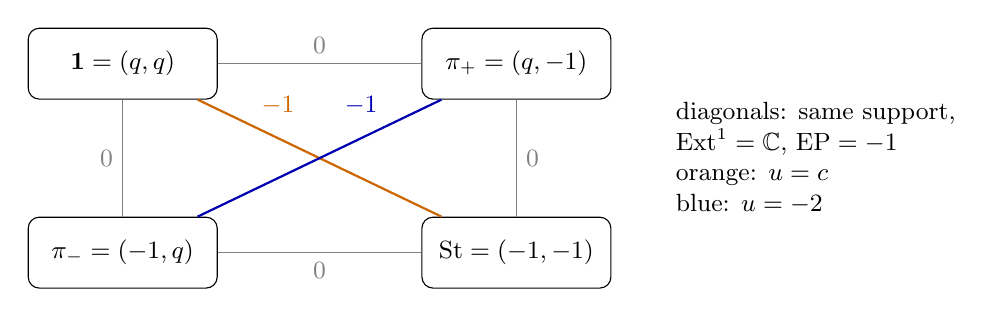
\begin{tikzpicture}[every node/.style={font=\small},>=Latex]
\node[draw,rounded corners,minimum width=2.4cm,minimum height=9mm] (t) at (0,2.4) {$\triv=(q,q)$};
\node[draw,rounded corners,minimum width=2.4cm,minimum height=9mm] (p) at (5,2.4) {$\pi_+=(q,-1)$};
\node[draw,rounded corners,minimum width=2.4cm,minimum height=9mm] (m) at (0,0) {$\pi_-=(-1,q)$};
\node[draw,rounded corners,minimum width=2.4cm,minimum height=9mm] (s) at (5,0) {$\St=(-1,-1)$};
\draw[gray] (t)--node[above]{$0$}(p);\draw[gray] (t)--node[left]{$0$}(m);
\draw[gray] (p)--node[right]{$0$}(s);\draw[gray] (m)--node[below]{$0$}(s);
\draw[thick,orange!80!black] (t)--node[pos=.22,above right]{$-1$}(s);
\draw[thick,blue!70!black] (p)--node[pos=.22,above left]{$-1$}(m);
\node[anchor=west,align=left] at (6.9,1.2) {diagonals: same support,\\ $\Ext^1=\mathbb C$, $\EP=-1$\\ orange: $u=c$\\ blue: $u=-2$};
\end{tikzpicture}
\caption{The four characters of the Hecke algebra of a quadratic block and their Euler--Poincar\'e pairings. Each has $\EP$ equal to $1$ with itself. Characters that differ in one coordinate are orthogonal. The two diagonals are the doubled fibers of the support map.}\label{fig:grid}
\end{figure}

\begin{example}[The elliptic norm of Steinberg by direct integration]\label{ex:norm}Since $\Theta_{\St}=-1$ on the elliptic set, $\EP(\St,\St)=1$ is the identity $\sum_T|W_T|^{-1}\int_T|\Delta_G(t)|\,dt=1$, with each elliptic torus of volume one. The two classes of unramified tori together contribute $(q^2-q+1)/(q^2+q+1)$. Each ramified quadratic extension contributes $q/(q^2+q+1)$. The total is $1$. For $\mathbb Q_3$ the three terms are $7/13,3/13,3/13$. For $\mathbb Q_5$ they are $21/31,5/31,5/31$. In the same way $|\Delta_G|\,|D_\eta|^2=4$ on the tori that split over $E_\eta$ gives $\|D_\eta\|^2_{\rm ell}=4$.
\end{example}
For the unramified computation, the norm-one group of $E$ maps onto the $q+1$ norm-one elements of the residue field, $|\Delta_G|=1$ off the classes of $\pm1$, and $|\Delta_G|=q^{-2n}$ on a shell of measure $(q-1)/((q+1)q^n)$ around each of $\pm1$. For a ramified extension, the Cayley parametrization $\lambda=\pm(1+y\sqrt\varpi)/(1-y\sqrt\varpi)$, $y\in\mathcal O$, gives $|\Delta_G|=q^{-2k-1}$ on the shell $v(y)=k$.

Later literature places these facts in a general theory: elliptic representations of Weyl groups \cite{Re01}, the elliptic and rigid cocenters \cite{CH17,CH21}, and extensions of tempered representations \cite{OS13}. In that language $\dim\ST^{\mathfrak s}=2$ is the number of elliptic conjugacy classes of $\mathbb Z/2*\mathbb Z/2$, the two classes of reflections.

\subsection{Examples and counterexamples over $\mathbb Q_3$ and $\mathbb Q_5$}\label{sub:counter}
\begin{center}\small
\begin{tabular}{@{}p{.36\linewidth}p{.27\linewidth}p{.27\linewidth}@{}}\toprule
Quantity & $F=\mathbb Q_3$ & $F=\mathbb Q_5$\\\midrule
$c=q+q^{-1}$ & $10/3$ & $26/5$\\
Quadratic characters & $\eta_2$ unramified, $\eta_3,\eta_6$ & $\eta_2$ unramified, $\eta_5,\eta_{10}$\\
Ramified quadratic block: $z=+1$, $z=-1$ & $\eta_6$, $\eta_3$ & $\eta_5$, $\eta_{10}$\\
Is $-1$ a square? & no & yes\\
Classes of elliptic tori & $2+1+1=4$ & $2+2+2=6$\\
$\Theta_{\St}(a(1+p^n))=2q^n-1$ & $5,17,53$ & $9,49,249$\\
$D_{\eta_2}$ on unramified tori, radius $n$ & $\pm2,\mp6,\pm18$ & $\pm2,\mp10,\pm50$\\
Depth-zero supercuspidals & $6$ & $8$\\
$d(\St)$, with $\vol(K_0)=1$ & $2$ & $4$\\
Example \ref{ex:cancel} & $\St-\pi_0^+-\pi_0^-$ & $\St-\pi(\theta)$, $\theta^3=1$\\\bottomrule
\end{tabular}
\end{center}
The second and third rows use $(3,3)_3=-1$, $(3,2)_3=-1$, $(5,5)_5=1$ and $(5,2)_5=-1$. When $-1$ is not a norm from a ramified extension, the two rational classes in a ramified torus are exchanged by the Weyl element, so there is one class of tori with trivial rational Weyl group.

The false implications, each with a witness:
\begin{enumerate}[leftmargin=*]
\item \emph{Supertempered does not imply cuspidal.} Steinberg: $J_{\St}=|t|$.
\item \emph{Cuspidal does not imply elliptic support.} A depth-zero supercuspidal: over $\mathbb Q_5$, $\Theta_{\pi(\theta)}(a(1+5^n))=5^n-1$.
\item \emph{Elliptic support does not imply ``in the span of the $D_\eta$.''} For a depth-zero supercuspidal $\pi$, the difference $\Theta_\pi-\Theta_{\pi^g}$ with $g=\diag(\varpi,1)$ vanishes on the split set because $g$ commutes with $A$. It is nonzero because $\pi^g$ has its type on $K_1$.
\item \emph{Elliptic representation does not imply supertempered character.} $\pi_\eta^+$.
\item \emph{An elliptic class need not have a tempered Jacquet-compatible representative.} $\tfrac12(\St-\triv)$.
\item \emph{Zero weak constant term does not imply local constancy of the split restriction}, and local constancy does not imply $\beta=0$. Steinberg, and Example \ref{ex:cancel}.
\item \emph{Tempered with vanishing regular density does not imply supertempered.} $\delta_I$ vanishes on the regular set, and its weak constant term in each block is the Plancherel density.
\item \emph{Decay of $h_D$ does not imply supertempered, outside virtual characters.} Take a wave packet $\int\Theta_{I(\chi_z)}g(z)\,dz$ with $g$ smooth. Its $h$ is given by the Fourier coefficients of $g$, which decay rapidly, and it is purely induced.
\item \emph{Elliptic support does not imply supertempered, outside virtual characters.} See the next example.
\end{enumerate}

\begin{example}[An elliptically supported distribution that is not supertempered]\label{ex:poisson}Let $F=\mathbb Q_5$ and $\pi=\pi(\theta)$ as in Example \ref{ex:cancel}. Let\[P(\vartheta)=\tfrac12+\sum_{n\ge1}q^{-n}\cos n\vartheta,\qquad L_P(Q)=\frac1{2\pi}\int_0^{2\pi}Q(2\cos\vartheta)P(\vartheta)\,d\vartheta .\]The function $P$ is a Poisson kernel. The moments of $L_P$ are $m_0=\tfrac12$ and $m_n=q^{-n}$. Put
\[
D=\Theta_{\St}-\Theta_\pi-D_{L_P}.
\]
By Example \ref{ex:cancel} and Theorem \ref{thm:decomp}(d) the normalized split restriction of $D$ is $q^{-|v(t)|}-q^{-|v(t)|}=0$ on all of $A_{\rm reg}$. So $D$ has elliptic support. It is invariant, has finite Bernstein support, is admissible by Theorem \ref{thm:finite-block-admissibility}, and is tempered in the smooth model. It is not supertempered: $D^w_B(a(t))=-q^{-|v(t)|}\ne0$. On the elliptic set $D=-1-\Theta_\pi$, so $D\ne0$. Over $\mathbb Q_3$ replace $\pi$ by $\pi_0^+\oplus\pi_0^-$.
\end{example}
The example shows that the restriction to virtual characters is essential in Corollary \ref{cor:three-questions}(c). It also shows that elliptic support is not a spectral condition on one block.

\subsection{A global characterization}\label{sub:global}
\begin{theorem}\label{thm:global}
Part (a) uses the inputs of Theorem \ref{thm:finite-block-admissibility}, and part (b) is conditional on the Schwartz trace identification.
Let $D$ be an invariant distribution on $G$ with finite Bernstein support. Write $D=\sum_{\mathfrak s}D_{L_{\mathfrak s}}+\Theta^{\rm st}$ with $\Theta^{\rm st}\in\ST(G)$.
\begin{enumerate}[label=(\alph*),leftmargin=*]
\item $D$ is admissible and locally representable.
\item $D$ is tempered if and only if every $L_{\mathfrak s}$ has polynomially bounded moments.
\item $D$ is center-finite if and only if every $L_{\mathfrak s}$ is a finite combination of jets, and a virtual character if and only if every $L_{\mathfrak s}$ is a finite combination of evaluations.
\item $D$ is supertempered, in the sense $D^w_B=0$, if and only if every $L_{\mathfrak s}=0$. Then $D$ is a virtual character.
\item $D$ is cuspidal if and only if in addition the Steinberg coefficient of $\Theta^{\rm st}$ is zero.
\item The normalized split restriction of $D$ is locally constant on $A$ if and only if $\Theta^{\rm st}$ satisfies Corollary \ref{cor:descent}.
\end{enumerate}
\end{theorem}
\begin{figure}[htbp]\centering
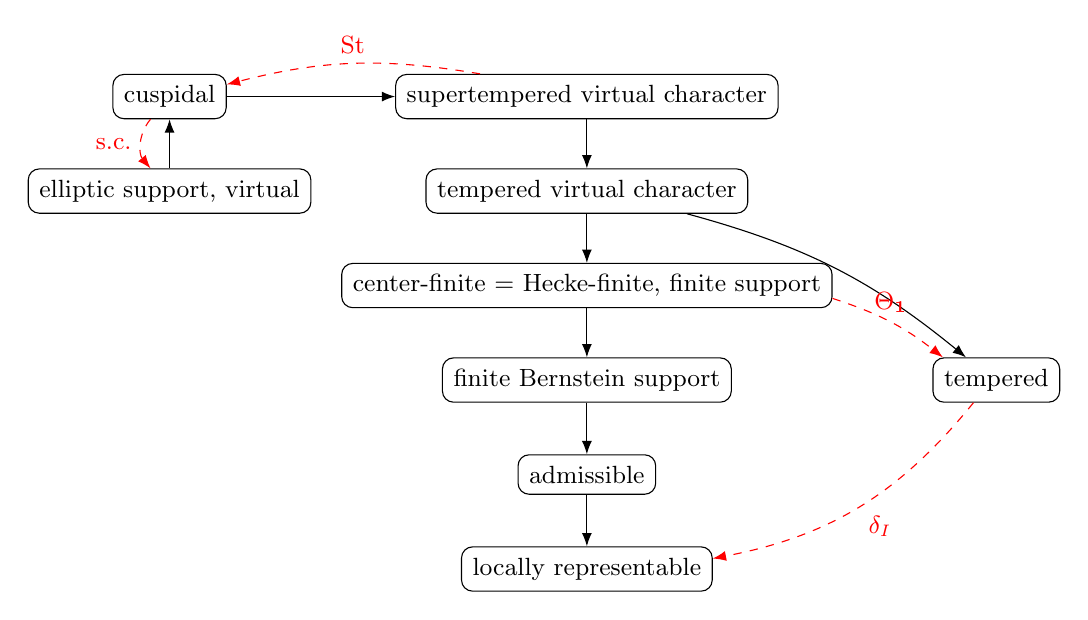
\begin{tikzpicture}[>=Latex,every node/.style={font=\small},bx/.style={draw,rounded corners,inner sep=4pt}]
\node[bx] (st) at (0,3.6) {supertempered virtual character};
\node[bx] (vc) at (0,2.4) {tempered virtual character};
\node[bx] (cf) at (0,1.2) {center-finite $=$ Hecke-finite, finite support};
\node[bx] (fb) at (0,0) {finite Bernstein support};
\node[bx] (ad) at (0,-1.2) {admissible};
\node[bx] (re) at (0,-2.4) {locally representable};
\node[bx] (cu) at (-5.3,3.6) {cuspidal};
\node[bx] (el) at (-5.3,2.4) {elliptic support, virtual};
\node[bx] (te) at (5.2,0) {tempered};
\draw[->] (st)--(vc);\draw[->] (vc)--(cf);\draw[->] (cf)--(fb);\draw[->] (fb)--(ad);\draw[->] (ad)--(re);
\draw[->] (cu)--(st);\draw[->] (el)--(cu);
\draw[->] (vc) to[bend left=12] (te);
\draw[->,dashed,red] (te) to[bend left=20] node[below right]{$\delta_I$} (re);
\draw[->,dashed,red] (cf) to[bend left=10] node[above]{$\Theta_{\triv}$} (te);
\draw[->,dashed,red] (st) to[bend right=12] node[above]{$\St$} (cu);
\draw[->,dashed,red] (cu) to[bend right=40] node[left]{s.c.} (el);
\end{tikzpicture}
\caption{Implications among the classes. Solid arrows are theorems above or in Section \ref{sec:descent}. Dashed red arrows are false, with the witness named.}\label{fig:global}
\end{figure}

\subsection{Open problems}\label{sub:st-open}
\begin{enumerate}[label=\arabic*.,leftmargin=*]
\item Describe all virtual characters with elliptic support. This needs the full supercuspidal character table on $A^0$ \cite{SS68,ADSS11}.
\item Decide whether $\delta_{\rm cusp}$ is admissible (Remark \ref{rem:infinite}).
\item Find tree formulas for the ramified $D_\eta$ through the Hecke algebra of a ramified quadratic block.
\item Develop the analog for the metaplectic double cover, where the $R$-groups and the Steinberg line both change.
\end{enumerate}

\subsection{Inputs and verification}\label{sub:st-status}
The results of this section are derived from the following classical inputs. For each input the exact statement and hypotheses still have to be checked against the source, except where noted.
\begin{center}\small
\begin{tabularx}{\linewidth}{@{}p{.42\linewidth}p{.2\linewidth}X@{}}\toprule
Input & Source & Used in\\\midrule
Tempered dual, reducibility, geometric lemma & \cite{GG63,Si79,Ca93} & Table \ref{tab:four}, Theorem \ref{thm:herb-rank-one}\\
Characters and Jacquet modules on contracting elements & \cite{Ca77} & Proposition \ref{prop:cass}\\
Local boundedness, local character expansion, $c_0$ and formal degree & \cite{HC99} & Theorems \ref{thm:herb-rank-one}, \ref{thm:germ}\\
Whittaker models and regular nilpotent orbits & \cite{Ro75} & table after Theorem \ref{thm:germ}\\
Herb's Theorems 2.5, 3.1, 3.2 (statements read) & \cite{He94} & Theorem \ref{thm:herb}\\
$R$-groups and the commuting algebra & \cite{Ke82} & Theorem \ref{thm:Deta}\\
Fixed-point character formula at level zero & \cite{SS97,Ko04} & Theorem \ref{thm:tree}, Proposition \ref{prop:sc}\\
Hecke algebras of the principal series blocks & \cite{Bo76,Ro98} & Proposition \ref{prop:EP}\\
Elliptic inner product and $R$-group formula & \cite{Ar93,Ka86,OS13} & Subsection \ref{sub:EP}\\\bottomrule
\end{tabularx}
\end{center}
Proposition \ref{prop:hecke} is proved in outline only. Remark \ref{rem:infinite} is heuristic. Theorem \ref{thm:decomp}(e) and Theorem \ref{thm:global}(b) are conditional on the Schwartz trace identification. The level-zero form of the Schneider--Stuhler formula was taken from the introduction of \cite{Ko04}. Its use is supported by the agreement of the resulting values for $\St$, $\triv$ and $\pi_\eta^\pm$ with the classical character formulas.


\section{Summary, limitations, and a comparison with metaplectic covers}\label{sec:summary}
This section collects the conclusions, the questions that remain open, and a comparison with the metaplectic case.

The reliable conclusions of this revision are as follows.  Smoothness and admissibility are distinct from continuity into a discrete automorphism group.  The normalized principal series has both quadratic and $|\cdot|^{\pm1}$ reducibility points.  Orbital-integral germs can compensate for discriminant factors, so singular vanishing cannot be inferred by inspection.  The trace transform is a transform of the \emph{invariant quotient}, and the Bernstein--Deligne--Kazhdan theorem requires regularity in unramified families, a uniform compact-open bound, and Grothendieck-group matching.  Conjugation-invariant linear functionals on the Hecke algebra are automatically distributions, and they form the algebraic dual of the trace image. Continuity becomes a condition only on larger spaces of test functions, where it is a growth condition on Laurent coefficients: none for polynomials, exponential for holomorphic functions, polynomial for smooth functions on the circle.  Supertemperedness is expressed by weak constant terms and does not imply literal support on the elliptic set. In rank one the supertempered virtual characters are spanned by the discrete series characters and the three quadratic differences, they split the elliptic quotient, and their behavior at $\pm I$ is governed by the trivial-orbit coefficient (Section \ref{sec:supertemp}).

The new spectral geometry, trace comparison, and duality sections establish polynomial uniqueness, algebraic trace restriction isomorphisms, instability of non-tempered evaluation, moment extension criteria, and central eigenfunctional formulas, subject to the stated classical representation-theoretic inputs. The following issues remain incompletely resolved:
\begin{enumerate}[label=\arabic*.,leftmargin=*]
\item The global topology of the Schwartz trace image, including fixed-level realizations (Remark \ref{rem:three-realizations}) and identification of the closed commutator kernel;
\item Descent beyond the principal-series block results, with the proper normalizations, and admissibility for infinite spectral support;
\item The proposed global analyticity criterion for invariant distributions from growth bounds on orbital data.
\end{enumerate}
The partial results and conditional formulations above do not settle these questions. Further proofs and independent verification are needed. The corresponding theory on a metaplectic double cover requires additional care: genuine characters, choices of splittings and measures, and the relevant intertwining and $R$-group data. This ordinary-group account should therefore remain a separate companion manuscript, not a theorem-by-theorem template assumed valid for covers.
\begin{example*}
The trivial character of $G=\mathrm{SL}_2(\mathbb Q_3)$ illustrates most of the distinctions made in the paper. In the unramified coordinates it is $(Q,d,b)\mapsto Q(\tfrac{10}3)-b$. It is an invariant distribution with finite Bernstein support, it is center-finite, and it is admissible. Its moments $3^n+3^{-n}$ grow exponentially, so it extends to the holomorphic spectral space and not to the smooth one. It is not tempered. Its normalized split restriction $|t-t^{-1}|$ takes the values $3^{-n}$ at $t=1+3^n$ and has no locally constant extension to $t=1$. Its values on tempered data are determined algebraically by the Steinberg trace and by the polynomial $Q$, and they do not depend continuously on them.
\end{example*}

\section*{Glossary}\label{app:glossary}
Each entry is a short reminder of the meaning of a term. The entries are independent of each other and of the numbering of the paper.
\begin{description}[style=nextline,leftmargin=1em]
\item[Admissible distribution] An invariant distribution that satisfies a local finiteness condition at every point: near the point it is annihilated by convolution with the idempotents of all representations of small compact open subgroups outside a restricted set. Characters of irreducible admissible representations are the basic examples. The term refers to distributions. It should not be confused with admissibility of a representation.
\item[Admissible representation] A smooth representation with finite-dimensional $J$-fixed spaces for every open compact subgroup $J$. For such a representation each operator $\pi(f)$ has finite rank, so the character $\tr\pi(f)$ is defined. Every irreducible smooth representation of a reductive $p$-adic group is admissible.
\item[Analytic spectral functional] A linear functional on trace polynomials that extends continuously to a space of holomorphic functions of the twisting parameter, with the topology of uniform convergence on compact sets. In rank one this holds exactly when the moments of the functional grow at most exponentially. Evaluation of the induced trace at a non-unitary parameter is an example.
\item[Bernstein center] The algebra of endomorphisms of the identity functor on smooth representations. It acts on every irreducible representation by a scalar that depends only on the supercuspidal support. It is the product, over the Bernstein components, of the rings of regular functions on their varieties, and it acts on distributions by duality.
\item[Bernstein component] A connected algebraic family of irreducible smooth representations organized using supercuspidal support and unramified twisting. For $\mathrm{SL}_2$ a component is either a single supercuspidal representation or the set of constituents of the principal series with a fixed inducing character on the units, up to inversion. The associated variety is a point, a copy of $\mathbb C^\times$, or its quotient by inversion.
\item[Center-finite distribution] A distribution whose translates under the Bernstein center span a finite-dimensional space. Such a distribution is supported on finitely many Bernstein components. In a component it is a finite combination of evaluations of the trace polynomial and of its derivatives, together with the exceptional coordinates.
\item[Cocenter] The quotient of the Hecke algebra by the span of the convolution commutators. This span equals the span of the differences of a function and its conjugates. Invariant distributions are exactly the linear functionals on the cocenter, and the trace transform is injective on it.
\item[Compact defect] The difference between the normalized split restriction of a character and its Jacquet-module character on the compact part of the split torus. Away from the compact part the two functions agree. The defect records the behavior of the character near the singular elements.
\item[Complementary series] The irreducible principal series representations induced from the real non-unitary characters $|\cdot|^s$ with $0<|s|<1$, in the normalization of this paper. They are unitarizable and not tempered. They show that the unitary dual is strictly larger than the tempered dual.
\item[Elliptic quotient] The Grothendieck group of finite-length representations modulo the classes of parabolically induced representations. For $\mathrm{SL}_2$ it is spanned by the supercuspidal classes, the three differences of quadratic constituents, and the class of the Steinberg representation. It has several natural splittings back into the Grothendieck group.
\item[Elliptic regular element] A regular semisimple element whose centralizer is anisotropic modulo the center. For $\mathrm{SL}_2$ these are the regular elements of the nonsplit maximal tori, whose eigenvalues lie in a quadratic extension and not in $F$.
\item[Extended quotient] For a finite group acting on a variety, the quotient of the set of pairs consisting of a group element and a point fixed by it. It contains the ordinary quotient and has extra components over the points with nontrivial stabilizer. The extra points are used to label the additional irreducible representations at reducible parameters.
\item[Fixed-level trace image] The set of trace forms of functions that are bi-invariant under a prescribed open compact subgroup. It is contained in the trace forms that vanish on representations without vectors fixed by that subgroup. Whether the two sets are equal depends on the subgroup.
\item[Hecke algebra] The convolution algebra of compactly supported locally constant complex-valued functions on $G$. It is the union of finite-dimensional subspaces of functions with prescribed support and level. For that reason every linear functional on it is continuous.
\item[Invariant distribution] A linear functional on the Hecke algebra that is unchanged when a test function is conjugated by an element of $G$. No separate continuity condition is needed. Characters, orbital integrals and evaluation at a central element are examples.
\item[Jacquet module] The representation of the torus on the $N$-coinvariants of a smooth representation, normalized by a modular character. It has finite dimension for a representation of finite length. Its character gives the character of the representation on the part of the split torus away from the compact subgroup.
\item[Local character expansion] The expression of a character near the identity as a finite combination of Fourier transforms of nilpotent orbital integrals on the Lie algebra. For $\mathrm{SL}_2$ there are five nilpotent orbits, the trivial orbit and four regular ones. The coefficient of the trivial orbit governs the behavior of the normalized character on the split torus near the identity.
\item[Normalized induction] Parabolic induction including the factor $\delta_P^{1/2}$. With this normalization unitary characters induce to unitarizable representations and the induced representations of a character and of its Weyl conjugate have the same constituents. The reducibility points depend on the normalization.
\item[Orbital integral] The integral of a test function over the conjugacy class of a regular semisimple element. The normalized orbital integral is the product with the square root of the absolute value of the Weyl discriminant. It can remain nonzero as the element approaches a singular one.
\item[Quasi-finite spectral type] A condition on a spectral functional supported on possibly infinitely many Bernstein components: its moments in each component are bounded by a polynomial, with one exponent for all components. Finite spectral type is the case of finitely many components. Without the common exponent the condition is called componentwise finite spectral order.
\item[Shalika germ] A function on the regular set near a singular element that gives the coefficient of a singular orbital integral in the asymptotic expansion of regular orbital integrals. The germs, and not the discriminant factor alone, decide whether a normalized orbital integral vanishes at a singular element.
\item[Spectral moment] The value of a spectral functional on a Laurent monomial in the twisting parameter, or on the symmetric combination $z^n+z^{-n}$ in a Weyl-invariant family. The sequence of moments determines the functional on the induced trace polynomial. Its rate of growth decides to which larger test spaces the functional extends.
\item[Supertempered virtual character] A finite linear combination of tempered irreducible characters whose normalized values decay rapidly on every Cartan subgroup. Equivalently, all of its weak constant terms vanish. For $\mathrm{SL}_2$ these are the combinations of discrete series characters and of the differences of the two constituents of a quadratic principal series.
\item[Tempered representation] An irreducible admissible representation occurring weakly in the regular representation; equivalently a representation satisfying the appropriate tempered matrix-coefficient bounds. Its character extends continuously to the Schwartz space. The trivial representation and the complementary series are not tempered.
\item[Trace Paley--Wiener theorem] The characterization of trace forms of Hecke-algebra elements by regularity under unramified twisting and uniform compact-open level bounds. It describes the image of the trace transform and not the image of the operator-valued Fourier transform. A version for the Schwartz space replaces regular functions by smooth functions on the unitary parameters.
\item[Weak constant term] The part of the normalized Jacquet-module character of a tempered representation that comes from the unitary exponents, not the entire Jacquet-module character. For the Steinberg representation the Jacquet-module character is nonzero and the weak constant term is zero.
\end{description}

\section*{Acknowledgments}
These notes were first written in November 1994 and were not published. In 2026 Argon (Gemini, Google) made a first, minor revision of the 1994 source. ChatGPT (Sol, OpenAI) refereed that revision and then wrote a second revision, an expository rewrite that responds to the referee report. That rewrite is Draft 1. Claude (Fable, Anthropic) prepared Draft 2. It brought the paper into line with the author's style guide, and it added the orienting paragraphs, the unnumbered examples, the literature review and these acknowledgments. It made no mathematical change to the existing statements and proofs.

In Draft 3 ChatGPT developed the spectral geometry, trace Paley--Wiener comparison, and continuous spectral duality sections, including the diagrams and elementary proofs. ChatGPT also developed the local finite-character interpolation theorem, conditional finite-block admissibility and split descent criterion, and the revised quasi-finite spectral definitions in Section 8. Claude (Fable, Anthropic) developed Section \ref{sec:supertemp} on supertempered distributions, including its proofs, examples and diagrams. The new sections preserve the distinction between established classical inputs and remaining verification tasks. 

ChatGPT refereed the main file of Draft 3. The five sections kept in separate source files, which contain most of the mathematics added in Draft 3, were not part of that review. Claude prepared Draft 4 in response to the report. It added Lemma \ref{lem:conj}, Proposition \ref{prop:alg-dual}, Theorem \ref{thm:three-duals} and the remarks and examples around them, specified the topologies of the Hecke algebra and of the Schwartz space, expanded the Introduction and the Glossary, and checked the bibliography. Claude also read the four sections written by ChatGPT for correctness. It found no error in them, and it could not check their cited inputs against the sources.

AI review is not an independent certification of the results. In particular, the first referee report and the revision that answers it were written by the same system, Section \ref{sec:supertemp} has been reviewed only by the system that wrote it, and the material added in Draft 4 has not been refereed. Further details on the AI usage can be found in the revision log, the file \texttt{revision\_log.md} that accompanies the source of this paper.

\begin{thebibliography}{ABPS14}
\bibitem[ABPS14]{ABPS14} A.-M. Aubert, P. Baum, R. Plymen and M. Solleveld, \emph{Geometric structure in smooth dual and local Langlands conjecture}, Japan. J. Math. \textbf{9} (2014), 99--136.
\bibitem[ABPS17]{ABPS17} A.-M. Aubert, P. Baum, R. Plymen and M. Solleveld, \emph{The principal series of $p$-adic groups with disconnected center}, Proc. London Math. Soc. \textbf{114} (2017), 798--854. \url{https://doi.org/10.1112/plms.12023}.
\bibitem[ABPS19]{ABPS19} A.-M. Aubert, P. Baum, R. Plymen and M. Solleveld, \emph{Smooth duals of inner forms of $\mathrm{GL}_n$ and $\mathrm{SL}_n$}, Doc. Math. \textbf{24} (2019), 373--420.
\bibitem[ADSS11]{ADSS11} J. D. Adler, S. DeBacker, P. J. Sally, Jr., and L. Spice, \emph{Supercuspidal characters of $\mathrm{SL}_2$ over a $p$-adic field}, in \emph{Harmonic Analysis on Reductive, $p$-adic Groups}, Contemp. Math. \textbf{543}, Amer. Math. Soc., 2011, 19--69. Available as arXiv:1012.5548.
\bibitem[AGS15]{AGS15} A. Aizenbud, D. Gourevitch and E. Sayag, \emph{$\mathfrak z$-finite distributions on $p$-adic groups}, Adv. Math. \textbf{285} (2015), 1376--1414. Available as arXiv:1405.2540.
\bibitem[AP24]{AP24} A.-M. Aubert and R. Plymen, \emph{Comparison of the Sally--Shalika character formulas with the endoscopic character identities for $\mathrm{SL}_2$}, preprint, arXiv:2410.20183.
\bibitem[Ar93]{Ar93} J. Arthur, \emph{On elliptic tempered characters}, Acta Math. \textbf{171} (1993), 73--138.
\bibitem[Ar94]{Ar94} J. Arthur, \emph{The trace Paley Wiener theorem for Schwartz functions}, Contemp. Math. \textbf{177} (1994), 171--180. \url{https://personal.math.ubc.ca/~cass/arthur/pdf/42.pdf}.
\bibitem[BDK86]{BDK86} J. Bernstein, P. Deligne, and D. Kazhdan, \emph{Trace Paley--Wiener theorem for reductive $p$-adic groups}, J. Analyse Math. \textbf{47} (1986), 180--192.
\bibitem[Bo76]{Bo76} A. Borel, \emph{Admissible representations of a semi-simple group over a local field with vectors fixed under an Iwahori subgroup}, Invent. Math. \textbf{35} (1976), 233--259.
\bibitem[Ca77]{Ca77} W. Casselman, \emph{Characters and Jacquet modules}, Math. Ann. \textbf{230} (1977), 101--105.
\bibitem[Ca93]{Ca93} W. Casselman, \emph{Introduction to the theory of admissible representations of $p$-adic reductive groups}, unpublished notes written 1974--1993, draft of May 7, 1993.
\bibitem[CH17]{CH17} D. Ciubotaru and X. He, \emph{Cocenters and representations of affine Hecke algebras}, J. Eur. Math. Soc. \textbf{19} (2017), no. 10, 3143--3177.
\bibitem[CH21]{CH21} D. Ciubotaru and X. He, \emph{Cocenters of $p$-adic groups, III: elliptic and rigid cocenters}, Peking Math. J. \textbf{4} (2021), no. 2, 159--186. Available as arXiv:1703.00378.
\bibitem[Cl91]{Cl91} L. Clozel, \emph{Invariant harmonic analysis on the Schwartz space of a reductive $p$-adic group}, in \emph{Harmonic Analysis on Reductive Groups} (Bowdoin, 1989), Progr. Math. \textbf{101}, Birkh\"auser, 1991, 101--122.
\bibitem[CT26]{CT26} T.-H. Chen and C.-C. Tsai, \emph{Admissibility of Bernstein centers}, preprint, arXiv:2608.21981 (2026).
\bibitem[Da00]{Da00} J.-F. Dat, \emph{On the $K_0$ of a $p$-adic group}, Invent. Math. \textbf{140} (2000), no. 1, 171--226.
\bibitem[De02]{De02} S. DeBacker, \emph{Homogeneity results for invariant distributions of a reductive $p$-adic group}, Ann. Sci. \'Ecole Norm. Sup. (4) \textbf{35} (2002), 391--422.
\bibitem[GG63]{GG63} I. M. Gelfand and M. I. Graev, \emph{Representations of a group of the second order with elements from a locally compact field}, Russian Math. Surveys \textbf{18} (1963), 29--100.
\bibitem[HC83]{HC83} Harish-Chandra, \emph{Supertempered distributions on real reductive groups}, in \emph{Studies in Applied Mathematics}, Adv. Math. Suppl. Stud. \textbf{8}, Academic Press, 1983, 139--153.
\bibitem[HC99]{HC99} Harish-Chandra, \emph{Admissible Invariant Distributions on Reductive $p$-adic Groups}, notes by S. DeBacker and P. J. Sally, Jr., University Lecture Series \textbf{16}, Amer. Math. Soc., 1999.
\bibitem[He94]{He94} R. A. Herb, \emph{Supertempered virtual characters}, Compositio Math. \textbf{93} (1994), no. 2, 139--154.
\bibitem[Ka86]{Ka86} D. Kazhdan, \emph{Cuspidal geometry of $p$-adic groups}, J. Analyse Math. \textbf{47} (1986), 1--36.
\bibitem[Ke82]{Ke82} C. D. Keys, \emph{On the decomposition of reducible principal series representations of $p$-adic Chevalley groups}, Pacific J. Math. \textbf{101} (1982), no. 2, 351--388.
\bibitem[Ko88]{Ko88} R. E. Kottwitz, \emph{Tamagawa numbers}, Ann. of Math. (2) \textbf{127} (1988), 629--646.
\bibitem[Ko04]{Ko04} J. Korman, \emph{A character formula for compact elements (the rank one case)}, preprint, arXiv:math/0409292 (2004).
\bibitem[LL79]{LL79} J.-P. Labesse and R. P. Langlands, \emph{$L$-indistinguishability for $\mathrm{SL}(2)$}, Canad. J. Math. \textbf{31} (1979), 726--785.
\bibitem[OS13]{OS13} E. Opdam and M. Solleveld, \emph{Extensions of tempered representations}, Geom. Funct. Anal. \textbf{23} (2013), no. 2, 664--714. Available as arXiv:1105.3802.
\bibitem[Re01]{Re01} M. Reeder, \emph{Euler--Poincar\'e pairings and elliptic representations of Weyl groups and $p$-adic groups}, Compositio Math. \textbf{129} (2001), 149--181.
\bibitem[Ro75]{Ro75} F. Rodier, \emph{Mod\`ele de Whittaker et caract\`eres de repr\'esentations}, in \emph{Non-Commutative Harmonic Analysis}, Lecture Notes in Math. \textbf{466}, Springer, 1975, 151--171.
\bibitem[Ro98]{Ro98} A. Roche, \emph{Types and Hecke algebras for principal series representations of split reductive $p$-adic groups}, Ann. Sci. \'Ecole Norm. Sup. (4) \textbf{31} (1998), 361--413.
\bibitem[Si79]{Si79} A. J. Silberger, \emph{Introduction to Harmonic Analysis on Reductive $p$-adic Groups}, Mathematical Notes \textbf{23}, Princeton Univ. Press, 1979.
\bibitem[So19]{So19} M. Solleveld, \emph{On completions of Hecke algebras}, in \emph{Representations of Reductive $p$-adic Groups}, Progr. Math. \textbf{328}, Birkh\"auser, 2019. Available as arXiv:1612.01776.
\bibitem[So24]{So24} M. Solleveld, \emph{Hochschild homology of reductive $p$-adic groups}, J. Noncommut. Geom. (2024), published online, DOI 10.4171/JNCG/556. Available as arXiv:2203.06435.
\bibitem[So25]{So25} M. Solleveld, \emph{Group algebras of reductive $p$-adic groups, their representations and their noncommutative geometry}, preprint, arXiv:2510.17260 (2025).
\bibitem[SS68]{SS68} P. J. Sally, Jr. and J. A. Shalika, \emph{Characters of the discrete series of representations of $\mathrm{SL}(2)$ over a local field}, Proc. Natl. Acad. Sci. USA \textbf{61} (1968), 1231--1237.
\bibitem[SS84]{SS84} P. J. Sally, Jr. and J. A. Shalika, \emph{The Fourier transform of orbital integrals on $\mathrm{SL}_2$ over a $p$-adic field}, in \emph{Lie Group Representations II}, Lecture Notes in Math. \textbf{1041}, Springer, 1984, 303--340.
\bibitem[SS97]{SS97} P. Schneider and U. Stuhler, \emph{Representation theory and sheaves on the Bruhat--Tits building}, Publ. Math. Inst. Hautes \'Etudes Sci. \textbf{85} (1997), 97--191.
\bibitem[SZ07]{SZ07} P. Schneider and E.-W. Zink, \emph{The algebraic theory of tempered representations of $p$-adic groups. Part I: Parabolic induction and restriction}, J. Inst. Math. Jussieu \textbf{6} (2007), no. 4, 639--688.
\bibitem[Ta83]{Ta83} M. Tadi\'c, \emph{The topology of the dual space of a reductive group over a local field}, Glas. Mat. \textbf{18} (1983), 259--279.
\bibitem[Ta92]{Ta92} M. Tadi\'c, \emph{Notes on representations of non-Archimedean $\mathrm{SL}(n)$}, Pacific J. Math. \textbf{152} (1992), 375--396.
\bibitem[Wa03]{Wa03} J.-L. Waldspurger, \emph{La formule de Plancherel pour les groupes $p$-adiques (d'apr\`es Harish-Chandra)}, J. Inst. Math. Jussieu \textbf{2} (2003), no. 2, 235--333.
\end{thebibliography}
\end{document}
